\documentclass{USC-Thesis}
\usepackage{graphicx}
\usepackage{amsmath}
\usepackage{amsfonts}
\usepackage{amssymb}
\usepackage{algorithm}
%\usepackage{algorithmic}
%\usepackage{algorithmicx}
\usepackage{algpseudocode}

\usepackage{hyperref}


\let\oldlistofalgorithms = \listofalgorithms
\renewcommand{\listofalgorithms}{  
\newpage
    \addcontentsline{toc}{chapter}{\listalgorithmname}
    \pagestyle{plain}
    \begin{singlespace} 
    \oldlistofalgorithms
    \end{singlespace}}

\begin{document}

\def\mytitle{Exploring and Mapping Confined and Sensor-Challenged Environments with Proprioception of an Articulated Mobile Robot}
\def\myauthor{Jacob Everist}
\def\bibliocommand{\bibliography{/Users/jse26711/Dropbox/dissertation}}
\title{\mytitle}

\author{Jacob Everist}
\major{Computer Science}
\month{April}
\year{2015}
\maketitle

\dedication
    \begin{quote}
        \raggedleft {\em to family}
    \end{quote}

\tableofcontents 	% Table Of Contents

\listoffigures	% List of figures

\listoftables	% List of tables

\listofalgorithms

\pagenumbering{arabic}


\topmatter{Preface}  % Preface with acknowlegements, etc.


Something sentimental here.


\topmatter{Abstract}


In many real-world environments such as flooded pipes or caves, exteroceptive sensors, such as vision, range or touch, often fail to give any useful information for robotic tasks. This may result from complete sensor failure or incompatibility with the ambient environment. We investigate how proprioceptive sensors can help robots to successfully explore, map and navigate in these types of challenging environments.

Our approach is to use a snake robot with proprioceptive joint sensors capable of knowing its complete internal posture. From this posture over time, we are able to sweep out the free space of confined pipe-like environments. With the free space information, we incrementally build a map. The success of mapping is determined by the ability to re-use the map for navigation to user-directed destinations.

We address the following challenges: 1) How does the robot move and locomote in a confined environment without exteroception? 2) How is the distance traveled by a snake robot measured with no odometry and no exteroception? 3) How does the robot sense the environment with only proprioception? 4) How is the map built with the information available? 5) How is the map corrected for visiting the same location twice, i.e. loop-closing? 6) How does the robot navigate and explore with the constructed map?

In order to move through the environment, the robot needs to have a solution for motion planning and collision-reaction. In an exteroceptive approach, we would detect and avoid obstacles at a distance. If collisions were made, touch sensors could detect them and we could react appropriately. With only proprioceptive sensors, indirect methods are needed for reacting to obstacles. A series of motion methods are used to solve these problems including compliant locomotion, compliant path-following, safe-anchoring, stability assurance, slip detection, and dead-end detection. We show results demonstrating their effectiveness.

While moving through the environment, the snake robot needs some means of measuring the distance traveled. Wheeled robots usually have some form of shaft encoder to measure rotations of the wheels to estimate distance traveled. In addition, range or vision sensors are capable of tracking changes in the environment to estimate position of the robot. GPS is not feasible because of its unreliable operation in underground environments. Our proprioceptive approach achieves motion estimation by anchoring multiple points of the body with the environment and kinematically tracking the change in distance as the snake contracts and extends. This gives us a rudimentary motion estimation method whose effectiveness we measure in a series of experiments.

Some method is needed to sense the environment. In an exteroceptive approach, vision and range sensors would give us a wealth of information about the obstacles in the environment at great distances. Touch sensors would give us a binary status of contact with an obstacle or not. With only proprioceptive joint sensors, our approach is to kinematically compute the occupancy of the robot’s body in the environment and record the presence of free space over time. Using this information, we can indirectly infer obstacles on the boundary of free space. We show our approach and the sensing results for a variety of environmental configurations.

Combining the multiple snapshots of the local sensed free space, the robot needs a means of building a map. In the exteroceptive approach, one would use the ability to sense landmark features at a distance and identify and merge their position across several views. However, in a proprioceptive approach, all sensed information is local. The opportunities for spotting landmark features between consecutive views are limited. Our approach is to use the pose graph representation for map-building and add geometric constraints between poses that partially overlap. The constraints are made from a combination of positional estimates and the alignment of overlapping poses. We show the quality of maps in a variety of environments.

In the event of visiting the same place twice, we wish to detect the sameness of the location and correct the map to make it consistent. This is often called the loop-closing or data association problem. In the case of exteroceptive mapping, this is often achieved by finding a correspondence between sets of landmark features that are similar and then merging the two places in the map. In the proprioceptive case, the availability of landmark features is scarce. We instead develop an approach that exploits the properties of confined environments and detects loop-closing events by comparing local environmental topologies. We show the results of loop-closing events in a variety of environmental junctions.

Once we have constructed the map, the next step is to use the map for exploration and navigation purposes. In the exteroceptive case, navigating with the map is a localization problem, comparing the sensed environment with the mapped one. This is also the approach in the proprioceptive case. However, the localization accuracy along the length of a followed path is more uncertain, so our path-following algorithms are necessarily more robust to this eventuality. In the exteroceptive case, the act of exploration can be achieved by navigating to the boundaries of the map with no obstacles. In the proprioceptive case, exploration is achieved by following every tunnel or path until a dead-end is detected. We show some environments that we successfully map and navigate, as well as some environments that require future work. 

\chapter{Introduction}
\label{introduction}

In this dissertation, we develop an algorithmic approach for robotically mapping confined environments using internal sensors only. Some challenging environments such as underground caves and pipes are impossible to explore and map with external sensors. Such environments often cause external sensors to fail because they are too confined, too hostile for the sensors, or incompatible to the fluid medium. These environments are also impossible for humans to explore for similar reasons. Robotic solutions are possible, but such environments often cause available external sensors to fail. A robotic solution that can explore and map without external sensors would allow access to previously inaccessible environments. 

For example, an approach that is invariant to ambient fluid (air, water, muddy water, etc.) would significantly impact cave exploration and underground science by the access to still deeper and smaller cave arteries regardless of whether they are submerged in water. Search and rescue operations would have additional tools for locating survivors in complicated debris piles or collapsed mines. Utility service workers would be able to map and inspect pipe networks without having to excavate or evacuate the pipes.

\section{Challenges}
\label{challenges}

\subsection{Limitations of Exteroceptive Sensors}
\label{limitationsofexteroceptivesensors}

Exteroceptive sensors are sensors that are affixed externally and designed to sense information about the robot's environment. They're biological equivalents include such things as vision, hearing, touch, taste and smell. The robot equivalents include touch, cameras, sonar, and laser range-finders.

Currently we cannot effectively explore and map these environments with exteroceptive sensors. Current state-of-the-art mapping methods depend on exteroceptive sensors such as vision, range, or touch sensors that are sensitive to the ambient properties of the environment. Sonar and laser-range finders are sensitive to the ambient fluid properties for which they are calibrated. They are also often ineffective due to occlusions, distortions, reflections, and time-of-flight issues. Changing visibility, lighting conditions and ambient fluid opacity impact the usefulness of vision sensors. Hazardous environments may also damage fragile external touch sensors.

\subsection{Tracking Position}
\label{trackingposition}

In addition to the challenges of sensing the environment, we also have the challenge of tracking the robot's position in the confined environment. Due to the enclosed nature of the environment, global positioning information is often unavailable. Therefore, any mapping method will need an accurate motion estimation approach for the robot. Wheeled dead-reckoning may be very difficult or impossible if the environment is highly unstructured or otherwise untenable to a wheeled locomotion approach. Even a well designed motion estimation approach will be susceptible to accumulation of errors and will require localization techniques that will reduce and bound the positional error of the robot.

\subsection{Proprioceptive Sensors}
\label{proprioceptivesensors}

Given these restrictions, developing an approach that will work on all the most challenging conditions forces us to rely on a strictly proprioceptive approach for collecting environmental information and building the map. Such proprioceptive sensors include accelerometers, gyros, INS (inertial navigation systems), and joint angle sensors. Examples of biological proprioception includes sense of hunger, fatigue, shortness of breath, pain, sense of hot, sense of cold, perceived configuration of the body, and numerous others.

Exteroceptive mapping approaches directly sense large sweeps of the environment at a distance and allow us to make multiple observations of environmental features from multiple poses, integrating this into a map. With a proprioceptive approach, the information is by definition internal to the robot's body and local to the robot's position. Any inferred information about the environment is limited to the immediate vicinity of the robot's pose. The challenge is to explore the environment and construct a map with fundamentally less information.

\subsection{Void Space and Features}
\label{voidspaceandfeatures}

Limited information about the immediate vicinity of an articulated robot can be obtained by sweeping the robot's body to cover all of the void space that is reachable. By taking posture snapshots while the robot is sweeping and plotting them into an image, we can create a rudimentary void space image of the local environment. The challenge then becomes how to utilize this particular type of data in a robotic mapping approach. 

In the exteroceptive approach (external sensors), one would use the ability to sense landmark features at a distance and identify and merge their position across several views. However, in a proprioceptive approach, all sensed information is local. Not only will the opportunities for spotting landmark features between consecutive views be limited, but we must also define what exactly we will use as landmark features. In exteroceptive mapping, the boundaries of the environment are sensed and landmark features are extracted that represent corners, curves, structures, and visual characteristics. With proprioceptive sensors, we present the different kinds of features that can be extracted and used from void space information.

\subsection{Map Representation}
\label{maprepresentation}

How is a map built and how is it represented? How can it be used and how accurate can it be? The map is built to void space data taken from proprioception. The map must be sufficiently accurate to navigate the environment to a given destination. What kinds of environmental characteristics can it capture and what are its limitations?

\subsection{Data Association}
\label{dataassociation}

In the event of visiting the same place twice, we wish to detect the sameness of the location and correct the map to make it consistent. This is often called the loop-closing or data association problem. In the case of exteroceptive mapping, this is often achieved by finding a correspondence between sets of landmark features that are similar and then merging the two places in the map. In the proprioceptive case, the availability of landmark features is scarce. The current best-practice methods for solving the data association problem depend on an abundance of landmark features with which multiple combinations of associations are attempted until an optimal correspondence is found. In our approach, with only a few landmarks to use, performing data association in this way becomes ineffective at best, destructive at worst. We determine a different approach to data association using void space information.

\section{Related Work}
\label{relatedwork}

The mapping of confined spaces is a recurring theme in the research literature. Work has been done to navigate and map underground abandoned mines [Thrun04] with large wheeled robots traveling through the constructed corridors. Although the environment is large enough and clear enough to make use of vision and range sensors, its location underground makes the use of GPS technologies problematic. This work can be applied to confined environments where exteroceptive sensors are still applicable.

Robotic pipe inspection has been studied for a long time [Fukuda89], but usually requires that the pipe be evacuated. The robotic solutions are often tailored for a specific pipe size and pipe structure with accompanying sensors that are selected for the task. Often the solutions are manually remote-controlled with a light and camera for navigation.

Other work has focused on the exploration of flooded subterranean environments such as sinkholes [Gary08] and beneath sea-ice or glaciers. This involves the use of a submersible robot and underwater sonar for sensing.

Other work has approach the problem of identifying features in the absence of external sensors. This work comes from the literature on robotic grasping and is described as “contact detection”. That is, the identification and reconstruction of object contacts from the joint sensors of the grasping end effector. Various methods to this approach are described in [Kaneko], [Grupen], [Haidacher], [Mimura].

Our earlier paper [Everist09] established the basic concept of mapping using void space information with a rudimentary motion estimation technique. This early work attempted to merge the information from contact detection with the new void space concept. We did not yet have an approach for localization, feature extraction, and data association.

Another researcher [Mazzini11] tackled the problem of mapping a confined and opaque environment of a pipe junction in an oil well bore hole deep underground where high temperature, high pressure, and mud make external sensors infeasible. Mazzini's approach focuses on mapping one local area of the underground oil well. They use physical probing with a robotic finger to reconstruct the walls of the pipe. The robot remains anchored and immobile so there are no need for motion estimation. Our dissertation differs from this work in that we use void space information instead of contact or obstacle information, our robot is mobile instead of anchored to one location, and that we are exploring and constructing a complete map instead of one local environment of interest.

\section{Approach}
\label{approach}

To address these challenges, our approach is to develop algorithmic methods for utilizing proprioceptive joint angle information on an articulated mobile robot to enable exploration and mapping of a confined environment. From a series of complete posture information sets, we build up void space information into a posture image and integrate it into a whole map. We hypothesize that with the posture images taken at multiple robot poses in the environment, we can integrate them into a map; we believe this approach will serve as effective alternative for mapping confined environments when exteroceptive sensors have failed or are unavailable.

Our claim here is that “the type of robot used and its method of locomotion are not important so long as the robot is articulated and with many joints”. The more joint sensors the robot has, the better capable the robot is of mapping.

In this design we use a simulator that enables us to rapidly develop and test different algorithmic techniques without becoming overly worried about the hardware and locomotive aspects of the robot. We use a simplified flat pipe-like environment with a snake robot that is capable of anchoring to the sides of the walls and pushing and pulling itself through the pipe on a near frictionless floor. 

We do not simulate any sensor-inhibiting fluid in the environment or sensor-failure scenarios, nor do use any type of external sensor, be it touch sensors, vision sensors, or range sensors such laser range-finders and sonar. Additionally, no global positioning system is used since it is not practical to expect GPS to function underground. The only sensors we permit ourselves to use are joint sensors.

For capturing the posture images, we examine a number of difficulties and pitfalls to capturing this information. Notably, the prevalence of slip of the robot can corrupt the posture image because the robot loses its stable frame of reference to the environment. We develop a number of techniques for safely capturing the void space information, reducing the likelihood of slip, detecting slip, and mitigating the damage if slip should occur.

We examine several possibilities for extracting landmark features from the posture images. We try several traditional forms of features such as corners and edges, but in the end we develop our own macro-feature which is the overall shape of the local environment captured by the posture image and reduced to the form of a medial axis.

When the robot is moving through the environment, we must also have techniques for estimating the motion between the poses at which we capture the posture images. We show a highly accurate but very slow method [Sec Motion 1] for our particular snake robot morphology, and compare it to a coarse but fast motion estimation method [Sec Motion 2]. We discover that the coarse method is sufficient so long as we rely on the macro-features of the posture images to constrain the possibilities.

Given these basics, we then delve into the heart of the matter: the actual integration of poses, motion estimates, and posture images into a coherent map. We develop and experiment with a few techniques using the constraints from the macro-features in a variety of ways [Sec Constrain 1]. We finally settle on an aggregate pose constraint method where the whole set of past poses is used to generate a feature that constrains the next pose [Sec Constrain 2].

We show how our mapping approach works in a variety of different environments for example, a single path pipe where there are no branches in the environment. The environment only contains a single path that includes a different variety of turns and angles. We then complicate matters by adding in different types of junctions such as T-junctions, Y-junctions, and X-junctions. We do not yet consider environments that have loops in them.

The adding of junctions adds significant complications and requires us to have a better understanding of the structure of our map. We establish a new type of mapping structure called a “shoot map”. A shoot is a section of the environment that is a single path. The shoot has an origin and a termination point which indicates either the boundary of the environment or more space yet to be explored. New shoots are created when a junction is detected, where the new shoot's origin is at the location of the parent shoot where the junction was detected. That representation allows us to deal with the restrictions on the type of information we can acquire and the often incompleteness of the posture image capture with respect to the actual local environment.

Finally, given the fundamental mapping structures and methods we have developed, we cast them into a probabilistic framework. This allows us to keep track of different map possibilities, discarding improbable ones, and selecting the most probable. Our mapping approach has certain ambiguities in the type of environmental information we can acquire. The probabilistic framework keeps track of these ambiguities until they can be resolved when more information is acquired.

\section{Experimental System}
\label{experimentalsystem}

Robot setup, joints and geometry, environmental parameters, simulation.

We explicitly chose to develop our approach in a simulation environment in order to rapidly develop a theoretical framework to the problem of mapping without external sensing. In future work, we will apply these techniques to physical robots.

We choose to use the Bullet physics engine (version 2.77) because it is free, open source, mature, and actively developed. Though it is primarily designed for games and animation, it is acceptable to our robotics application. Our primary requisites are simulation stability and accurate modeling of friction and contact forces. True friction and contact modeling are not available to us without specially designed simulation software at a monetary and performance speed cost. Our choice of Bullet gives us believable results so long as we do not demand too much and try to simulate challenging situations (e.g. high speed, high mass, 1000s of contact points).

\begin{figure}[htbp]
\centering
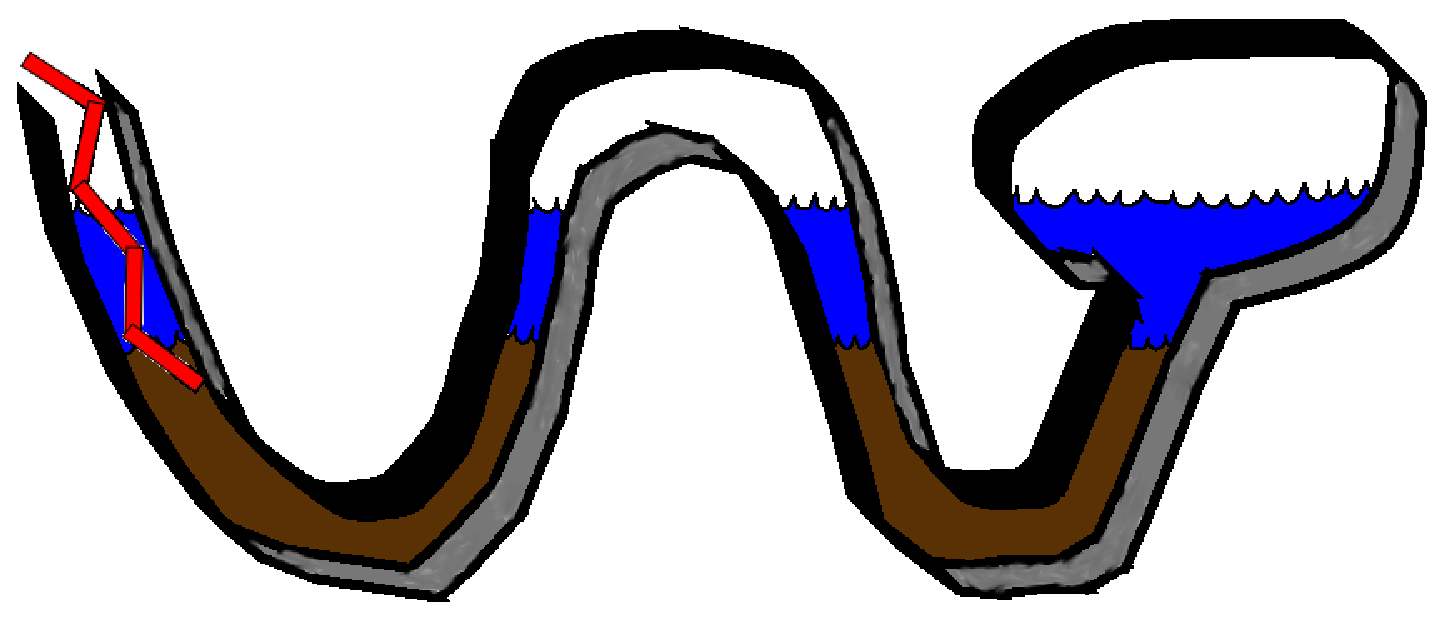
\includegraphics[keepaspectratio,width=400pt,height=0.75\textheight]{rectv2-red.eps}
\caption{Example environment.}
\label{env1}
\end{figure}



We focus our attention on environments such as the one depicted in \autoref{env1}. We build a flat plane and place a number of vertical walls to create a pipe-like maze environment. All environments we study are flat and have no vertical components. This means we need only focus on building 2D maps to represent the environment. From here on in this paper, we refer to such environments as pipes even though they may not correspond to the even and regular structures of physical utility pipes.

A snake robot is placed in the pipe environment as shown in \autoref{env1}. The snake robot consists of regular rectangular segments connected by actuated hinge joints. Each of the joint axes is parallel and coming out of the ground plane. This means the snake has no means to lift its body off the ground because all of its joints rotate in the plane of the ground. It is only capable of pushing against the walls and sliding along the ground. We choose a reduced capability snake robot because we wish to focus on the mapping problem instead of the more general serpentine control problem.

\begin{figure}[htbp]
\centering
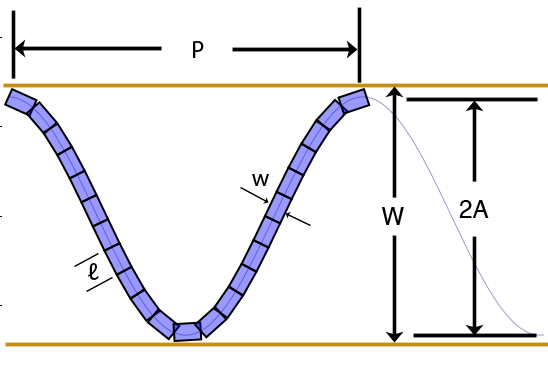
\includegraphics[keepaspectratio,width=400pt,height=0.75\textheight]{CurveDiagram.png}
\caption{Definitions of snake and pipe parameters.}
\label{env2}
\end{figure}



We can parameterize the snake and the pipe environment. For the snake robot, $l$ is the snake segment length, $w$ is the segment width, $N$ is the number of segments connected by $N-1$ joints, and $m$ is the maximum torque capable by each of the joint motors. 

 \cite{Vona:2010p391} 

For the environment, we can begin by defining the pipe width $W$. For a pipe with parallel and constant walls, this is a straightforward definition as seen in \autoref{env2}. For non-regular features, we define the pipe width at a given point on one wall to be the distance to the closest point on the opposing wall. This correctly captures the fact that a robot that is wider than the smallest pipe width $W$ will be unable to travel through that smallest width and will create a non-traversable pinch point. Conversely, a pipe width $W$ that is larger than the reach of a robot will become a void space that the robot will have difficulty completely sensing without the aid of external sensors. For both the minimum and maximum pipe widths of a given environment, we define $W_{min}$ and $W_{max}$ respectively where $W_{min} \leq W_i \leq W_{max}$ where $W_i$ is the pipe width at some point on wall $p_i$ of the pipe environment.

Each joint on the robot is actuated by a motor and PID controller. It can actuate the joint anywhere from $\pm160$ degrees. It uses the built-in motor capabilities of Bullet that allows us to set the joint angular velocity at run-time. Therefore, all outputs of the PID controller set velocity commands to the joint and the physics engine does its best to satisfy those as velocity constraints. 


\begin{algorithm}
\caption{PID Controller}          % give the algorithm a caption
\label{alg1}
\begin{algorithmic}

\State $\epsilon \Leftarrow (\alpha - \phi)$

\If{$| \epsilon | > \mathrm{tol} $}

  \State $\epsilon_{sum} \Leftarrow \epsilon_{sum} + \delta t \times \epsilon$
  \State $\delta \epsilon \Leftarrow \epsilon-\epsilon_{last}$
  \State $\epsilon_{last} \Leftarrow \epsilon$
  \State $\hat{v} \Leftarrow \mathrm{P} \times \epsilon +\mathrm{I} \times \epsilon_{sum}+\mathrm{D} \times \delta \epsilon/\delta t$ 

  \If{$\hat{v} > v_{max}$}
    \State $\hat{v} \Leftarrow v_{max}$
  \EndIf
  \If{$\hat{v} < -v_{max}$}
    \State $\hat{v} \Leftarrow -v_{max}$
  \EndIf


\EndIf

\end{algorithmic}
\end{algorithm}


The structure of the PID controller is shown in Algorithm \autoref{alg1}. Line 1 defines the error as the difference between the target and the actual joint angle. Line 2 prevents the controller from executing if the error falls below an acceptable threshold. This prevents the motor from attempting to perform minor corrections to an already near-correct angle in order to avert oscillations or error-producing compensations. Line 3 is the summation term for error over time while line 4 and 5 is the instantaneous error change from the previous controller iteration. The actual PID control law is shown on line 6 where P is the proportional term coefficient, I is the integration term coefficient, and D is the derivative term coefficient. The result outputs a command velocity for the Bullet engine. Finally, lines 7--10 limit this velocity to a maximum.

Each of the joints gives angle position information to simulate a shaft encoder or potentiometer. For this study, we do not simulate calibration error, sensor noise, resolution error, or gear backlash. Calibration error has been studied elsewhere \slash cite and there exists correction mechanisms for it. In the case of sensor noise, the noise on potentiometers is small enough not to affect our algorithms. Gear backlash was encountered and studied in \slash cite Mazzini. The primary error of concern is resolution error caused by the discretization process of a shaft encoder or an A\slash D converter. This problem has been studied \slash cite. Given a sensitive enough A\slash D converter (really?), this problem can be eliminated. In this study, we assume correct and noise-free joint sensors.

A joint provides an API to the controlling program with 2 read-write parameters and 1 read-only parameter. The read-write parameters are the target joint angle $\alpha_i$ and the maximum torque $m_i$, with the actual angle $\phi_i$ being the read-only parameter. $\alpha_i$ is the angle in radians that we desire the joint to rotate to. $\phi_i$ is the actual angle of the joint that reflects the current physical configuration of the robot. $m_i$ is the maximum permitted torque that we wish to limit the individual motors to. The maximum torque can be lowered to make the joints more compliant to the environment.

\pagebreak 

\chapter{Sensing Space}
\label{chap:sensing}

\section{Problem}
\label{sensing:problem}

Need to argue here that we are forced to use a contact sensing modality. However, existing contact sensing solutions only return contact point data, i.e. point and location of the boundary. Whereas, with range-based solution, both boundary and void space information are returned. Mostly void space in fact.

Types of sensing can be classified with the following table. The biological senses are grouped with their analogous robotics counterparts.



\begin{center}
    \begin{tabular}{| c | p{5cm} | p{5cm} |}
    \hline
        & Biology   & Robotics \\ \hline
    Exteroception & sight, hearing, touch, taste, smell & camera, sonar, LIDAR, tactile \\ \hline
    Interoception & hunger, hot, cold, thirst, pain & battery sensor, temperature \\ \hline
    Proprioception & relative positions of neighboring parts of the body, strength of effort & joint sensor, strain sensor, current sensor, accelerometer, gyros, INS \\ \hline
    \end{tabular}
\end{center}


For the mapping problem, we are going to need a lot of data to build a map of the environment. Existing contact solutions that rely on proprioception such as finger probing and geometric contact detection are too time-consuming to extract data in large volumes. Similarly, other contact sensing solutions such as bump sensors, whiskers or tactile surfaces give more uncertain and noisy contact data while still being time-consuming.

The existing contacts detection approaches that use proprioception are based in the robotic manipulation literature. An end effector as affixed to an arm affixed to ground in an operational workspace. Contact points are inferred from a combination of the choice of motion, the proprioceptive sensors, and the geometry of the robot. The two major approaches are geometric contact detection and finger probing. The first slides the linkage of the arms along a surface to be detected and reconstruct the contact points from the joint values. The latter infers the contact point from the halting of motion of the end effector along a linear path.

We observe that none of the existing contact sensing solutions emphasize extracting void space as part of their sensing roles. We recognize that in the absence of a range sensor to provide void space data, we can use the body of the robot to extract void space instead. In fact, void space data is extracted in significantly more volumes that it becomes practical to use contact sensing solution to build maps. In this dissertation, we build maps primarily with void space data. We use a rough collision detector to detect dead-ends and is our only instance using any boundary information.

The ratio of the volume of boundary information to void space information can be modeled by the scan angle of a particular range sensor. For a particular scan angle, volume of information can be modeled as number of pixels for some pixel resolution. The number of pixels of void space and boundary can be computed from the area and arc length of a fraction of a circle.

For some scan angle $\theta$ and some boundary range $r$, the arc length $L$ and area $A$ is:


\begin{equation*}
L = r \theta
\end{equation*}
\begin{equation}
A = \frac{r^2 \theta}{2} 
\end{equation}


For some pixel size $p_d$, the ratio of the volume of void space to the volume of boundary is:


\begin{equation*}
\frac{A}{L*d_p}  = \frac{2 * r * \theta}{r^2 * \theta * d_p} = \frac{2}{r * d_p} 
\end{equation*}


We can see, for any reasonable set of values, a range sensor provides far more void space data than boundary data. For instance, for $r=10.0$ and a pixel width of $d_p = 0.1$, the ratio of void space to boundary data is $\frac{2}{r * d_p}= 2$. This void space data is often used in many SLAM techniques. Therefore, in a contact-based mapping approach, it would be reasonable to seek out some way to find the comparable void space data for contact sensing and exploit it.

For our particular sensing approach, we chose to use proprioceptive sensors because we want to use the intrinsic geometry of the robot's body as the sensor. For any confined environment, it will be difficult to find the workspace to deploy many of the extended contact sensing approaches such whiskers or probes and use them effectively. Furthermore, a specifically designed external contact sensors such as tactile surfaces or bump sensors will see repeated and near-constant use and may give overly noisy and uncertain data coupled with hastened wear-and-tear. Any approach that uses the existing robot body and does not depend on adding more sensors will be of great use to sensor-challenged and confined environments with existing robots unaugmented.

Our approach is to use the body of the robot to sweep the space of the environment and build up a model of the void space of the environment. From this void space, we can build up a map of the environment without explicitly sensing the obstacles and boundary. We focus on identifying, not where the obstacles are, but where they are not. Through this, we hope to extract the maximum amount of information about the environment with the minimal amount of sensors and action.

\section{How to Sense}
\label{howtosense}

We use a common sense assumption that the robot's body can never intersect with an obstacle. We call this the Obstacle-Exclusion Assumption. If we take the corollary of this assumption, we conclude that all space that intersects with the robot's body must be free space. If we record the robot's body posture over time, we can use this to build a map of the local environment's free space.

We need 3 key ingredients to build an accurate map of the free space in the local environment: 1) known geometry of the robot's rigid body linkages, 2) accurate joint sensors for computing kinematics, and 3) an accurate reference pose to the global frame. If all of these things are available, we can build a local map such as shown in \autoref{pokebehavior}.

\begin{figure}[htbp]
\centering
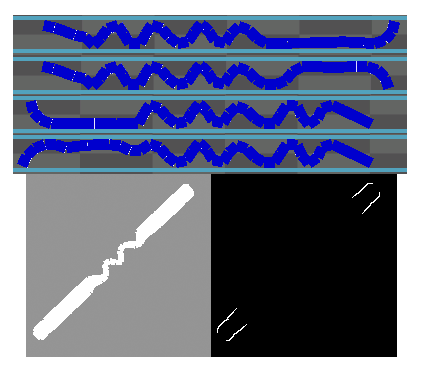
\includegraphics[keepaspectratio,width=400pt,height=0.75\textheight]{PokeBehavior.png}
\caption{TODO: Remove the obstacle map. Free space map from PokeWalls behavior.}
\label{pokebehavior}
\end{figure}



The map is achieved by rigidly anchoring to the environment and maintaining a set of stable reference poses. One side of the snake's body is used to sweep the free space, making multiple snapshots of the robot's posture over time and plotting them into a map. We discuss each aspect of our approach and show the results for a variety of environmental configurations.

The key point here is that sensing cannot be accomplished without action. Action by itself runs the risk of disturbing the environment or causing errors in the reference pose. Though sensing cannot be accomplished without action, action runs the risk of modifying the result. Special care must be taken that the risk of modifying the environment is minimized. Here, we include the robot's body in our definition of the environment so that anchor slippage is a form of environment modification.

As part of the action, at each instance of time $t$, we produce a posture vector $\bar{phi}_t$, representing the state of the joint angle sensors of the robot such that:


\begin{eqnarray}
\bar{\phi}_t = { \phi^t_1, \phi^t_2, … , \phi^t_{M-1}, \phi^t_M}
\end{eqnarray}


Over a series of time, we produce a series of posture vectors called the posture sequence:


\begin{eqnarray}
\bar{\Phi}_{1:t} = { \bar{\phi}_1, \bar{\phi}_2, … , \bar{\phi}_{t-1}, \bar{\phi}_t}
\end{eqnarray}


Using kinematics and geometry of the robot over time, we can produce the posture image $I_{k}$ which represents the swept void space at the position and orientation $X_{k}$ in the global environment.

\section{Posture Image}
\label{postureimage}

Using the control method shown in Control chapter to sweep out the void space of the local environment, we show how we capture sensor data and process it for consumption for our later mapping algorithms.

\subsection{Data Capture}
\label{datacapture}

Once the posture of the snake has stabilized and the anchor points give us good reference poses to the global frame, our objective is take the posture vector, $\bar{\phi_t}$ at time $t$, and convert it to a 2D spatial representation of free space, $M_p$ at the current pose $p$. We separate the tasks of spatial representation and positioning the data in the global frame. To do this, we create a local map centered on the robot's body on which the spatial data is plotted while the robot remains in one position.

The local map is an occupancy grid representation where each cell of the grid has two states: \emph{unknown} or \emph{free}. If the body of the robot is present on a cell, this cell is marked \emph{free}. Otherwise, it is \emph{unknown}. It is unknown instead of \emph{occupied} because our approach does not have any means to specifically observe obstacles beyond contact detection heuristics. The heuristics are not accurate enough to plot their positions into the occupancy grid, so we leave the cells unknown for now.

The size of a cell is chosen for the desired accuracy we require. Smaller cell sizes require more computational time, but larger cell sizes will result in blocky maps. We choose our cell dimensions $s_p \times s_p$ to be $s_p = \frac{l}{3} = 0.05$, or one third the length of a snake segment.

Given that we now have our cell dimensions, we can compute the dimensions of our local map to be 


\begin{eqnarray}
\label{eqn:mapSize}
s_M = l * N + 4
\end{eqnarray}


where $l$ is the segment length and $N$ is the number of segments. $s_M$ is the maximum length from the origin at the center of our local coordinate system. We want the dimensions to be larger than the worse case scenario of the snake's posture. We also include an extra padding of $4$ to ensure that the snake never reaches the boundary of the grid.

The number of cells or pixels in our local map will be $n_p \times n_p$ where 


\begin{eqnarray}
\label{eqn:numPixels}
n_p = \bigg\lceil \frac{2 s_M}{s_p} + 1 \bigg\rceil
\end{eqnarray}


This equation ensures that $n_p$ is an odd integer. The $+1$ factor adds an extra cell whose center will act as the origin of our local coordinate system.

Now that we have the dimensions of the grid space and its relation to Cartesian space, we need to know how to convert points from one space to the other. To convert a grid index $(i_x,i_y)$ to Cartesian space point $(p_x,p_y)$ centered within the cell, we compute the following:


\begin{eqnarray}
\label{eqn:g_to_p}
p_x = \bigg(i_x - \bigg\lfloor\frac{n_p}{2}\bigg\rfloor \bigg)\frac{s_p}{2} \\
p_y = \bigg(i_y - \bigg\lfloor\frac{n_p}{2}\bigg\rfloor \bigg)\frac{s_p}{2}
\end{eqnarray}


Conversely, to find the index of a cell $(i_x,i_y)$ that contains a Cartesian point $(p_x,p_y)$, we compute the following:


\begin{eqnarray}
i_x = \bigg\lfloor \frac{p_x}{s_p} \bigg\rceil + \bigg\lceil\frac{n_p}{2}\bigg\rceil \\
i_y = \bigg\lfloor \frac{p_y}{s_p} \bigg\rceil + \bigg\lceil\frac{n_p}{2}\bigg\rceil
\end{eqnarray}


Now that we have the tools for mapping positions in physical space to our grid space occupancy map, we need data to plot into the map. Using kinematics, we compute the geometry of the posture of the snake. We can represent this by a 4-sided rectangle for each segment of the snake. We set the origin of our coordinate system on segment 19 and joint 19 which is the midway point for $N = 40$. We define this to be:


\begin{equation}
O_t = (x_{19}, y_{19}, \theta_{19}) = (0, 0, 0)
\end{equation}


where $O_t$ is the pose of $P_{19}$ in the local frame at time $t$. This may change which is explained in \autoref{sec:ref_stable}.

To compute the segment 19 rectangle, starting from the origin for $k = 19$, $x_k = 0$, $y_k = 0$, and $\theta_k = 0$, we compute the following:


%From 19, towards N
\begin{equation}
\label{equ:rect1}
\begin{array}{l}
\displaystyle x_{k+1} = x_k + l \cos(\theta_k) \\
\displaystyle y_{k+1} = y_k + l \sin(\theta_k) \\
\displaystyle \theta_{k+1} = \theta_k - \phi_{k+1} \\
\displaystyle p_1 = \bigg( x_{k+1} - \frac{w\sin(\theta_k)}{2} , y_{k+1} + \frac{w\cos(\theta_k)}{2}\bigg) \\
\displaystyle p_2 = \bigg( x_{k+1} + \frac{w\sin(\theta_k)}{2}, y_{k+1} - \frac{w\cos(\theta_k)}{2} \bigg) \\
\displaystyle p_3 = \bigg( x_{k+1} - l\cos(\theta_k) + \frac{w\sin(\theta_k)}{2}, y_{k+1} - l\sin(\theta_k) - \frac{w\cos(\theta_k)}{2} \bigg) \\
\displaystyle p_4 = \bigg( x_{k+1} - l\cos(\theta_k) - \frac{w\sin(\theta_k)}{2}, y_{k+1} - l\sin(\theta_k) + \frac{w\cos(\theta_k)}{2} \bigg) \\
\displaystyle R_k = (p_4,p_3,p_2,p_1)
\end{array}
\end{equation}


The result is the rectangle polygon $R_k$, which represents the rectangle of the segment $19$. The next reference pose $(x_{k+1},y_{k+1},\theta_{k+1})$ is also computed. Here $k+1=20$. To compute the k\textbackslash{}textsuperscript\{th\} rectangle for $k \geq 19$, we need only compute this iteratively until we reach the desired segment.

To perform this backwards, to find segment $18$, where $k+1=19$ and $(x_{k+1}, y_{k+1}, \theta_{k+1}) = O_t$, we compute the following:


\begin{equation}
\label{equ:rect2}
\begin{array}{l}
\displaystyle \theta_k = \theta_{k+1} + \phi_k \\
\displaystyle x_k = x_{k+1} - l \cos(\theta_k) \\ 
\displaystyle y_k = y_{k+1} - l \sin(\theta_k) \\
\displaystyle p_1 = \bigg( x_{k+1} - \frac{w\sin(\theta_k)}{2} , y_{k+1} + \frac{w\cos(\theta_k)}{2}\bigg) \\
\displaystyle p_2 = \bigg( x_{k+1} + \frac{w\sin(\theta_k)}{2}, y_{k+1} - \frac{w\cos(\theta_k)}{2} \bigg) \\
\displaystyle p_3 = \bigg( x_{k+1} - l\cos(\theta_k) + \frac{w\sin(\theta_k)}{2}, y_{k+1} - l\sin(\theta_k) - \frac{w\cos(\theta_k)}{2} \bigg) \\
\displaystyle p_4 = \bigg( x_{k+1} - l\cos(\theta_k) - \frac{w\sin(\theta_k)}{2}, y_{k+1} - l\sin(\theta_k) + \frac{w\cos(\theta_k)}{2} \bigg) \\ 
\displaystyle R_k = (p_4,p_3,p_2,p_1)
\end{array}
\end{equation}


The result is the same polygon as well as the new reference pose for segment $18$. To compute the k\textbackslash{}textsuperscript\{th\} segment rectangle for $k < 19$, we need only use this equation iteratively. Computation of all $N$ rectangles results in the set of rectangles $\bar{R_t}$ for the current posture.

Now that we have a set of rectangles which represent the geometry of the robot in its current posture, we want to plot its occupied space into the local occupancy map. To do this, we need to convert polygons in Cartesian space into sets of grid points. To do this, we use a point-in-polygon test algorithm for each of the pixels in the map.

The simplest approach is as follows. For each pixel, convert it to Cartesian space, test if it's contained in any of the polygons, and if it is, set the pixel to \emph{free}. Otherwise, let the pixel remain in its current state. The pseudocode for the point-in-polygon test for convex polygons derived from \textbackslash{}cite\{orourke98\} is seen in Algorithm \autoref{alg:pip_test}.


\begin{algorithm}
\caption{Point-in-Polygon Test}          % give the algorithm a caption
\label{alg:pip_test}
\begin{algorithmic}

\State $R \Leftarrow $ rectangle
\State $P \Leftarrow $ point

\For{$i = 0 \to 4$}
\State $A_x \Leftarrow R[i \bmod 4][0] $
\State $A_y \Leftarrow R[i \bmod 4][1] $
\State $B_x \Leftarrow R[(i+1) \bmod 4][0] $
\State $B_y \Leftarrow R[(i+1) \bmod 4][1] $
\State $C_x \Leftarrow P[0] $
\State $C_y \Leftarrow P[1] $

\If{$!((Bx - Ax) * (Cy - Ay) - (Cx - Ax)*(By - Ay) \geq 0)$}
\State return False
\EndIf
\EndFor
\State return True

\end{algorithmic}
\end{algorithm}


\begin{figure}[htbp]
\centering
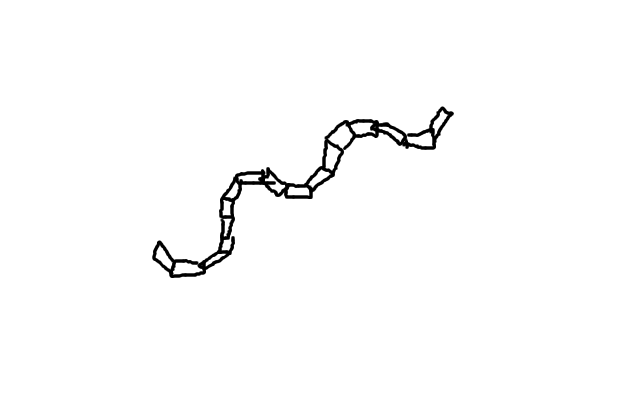
\includegraphics[keepaspectratio,width=400pt,height=0.75\textheight]{4_snapshot_1.png}
\caption{Snapshot of $\bar{\phi_t}$ in local coordinates.}
\label{snapshot}
\end{figure}



A single snapshot of the snake posture plotted into the local map is shown in \autoref{snapshot}. The posture $\bar{\phi_t}$ is captured, the rectangles $\bar{R_t}$ representing the body segments are computed from kinematics, each pixel $(i_x,i_y)$ of the map $M_p$ is converted to Cartesian space point $(p_x,p_y)$ and checked by the point-in-polygon algorithm if it is in a rectangle $R_k$. If it is, $M_p(i_x,i_y)$'s value is set to \emph{free}. This is repeated for each point in each rectangle for a posture snapshot at time $t$.

\begin{figure}[htbp]
\centering
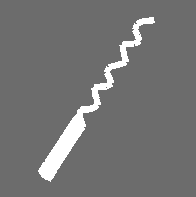
\includegraphics[keepaspectratio,width=400pt,height=0.75\textheight]{localOccMapSingle0.png}
\caption{Single forward sweep.}
\label{single_sweep}
\end{figure}



\begin{figure}[htbp]
\centering
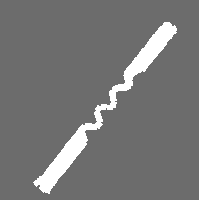
\includegraphics[keepaspectratio,width=400pt,height=0.75\textheight]{localOccDouble.png}
\caption{Forward and backward sweep.}
\label{double_sweep}
\end{figure}




While running the PokeWalls behavior, we periodically take snapshots at the conclusion of each Transition step and plot them into the map. A complete sweep with the PokeWalls behavior is shown in \autoref{single_sweep}. Furthermore, if we also perform a sweep with the other side of the snake, we can get a map like \autoref{double_sweep}.

Notice in \autoref{double_sweep} that there is a gap in the free space data in the center of the body. These segments at the center remain immobilized throughout the sweeping process and never give extra information. This gap in the center is our ``blind spot'' for this configuration. It is necessary that the center remain immobilized to ensure anchors do not slip so that we maintain correct reference poses to the global frame.

We have no guarantee that there are obstacles at the boundaries of our free space map. We also have no quick way to determine if the boundary of our map is an obstacle or a frontier. While the boundaries at the front and back are usually assumed to lead to more free space, anywhere along the sides could be a missed side passage that the snake failed to discover due to it being too small or being in our blind spot. To combat this situation, we either must perform laborious and time-consuming contact probing of every surface, or use quick-and-dirty contact detection heuristics to guide our mapping process.

\section{Data Processing}
\label{dataprocessing}

Once we have the raw sensor data successfully plotted into a local occupancy map, we must convert this data into a form that is useful for our mapping algorithms. Here, we present three different forms of data processing that we use in our approach.

\subsection{Convex Hull}
\label{convexhull}

One way we process our free space data is by taking its convex hull. In theory, this would create some smooth boundaries and can plausibly represent the true local space under some certain conditions. The definition of the convex hull is, given a set of points $P$, find the convex polygon $H$ with minimum area that contains all of $P$.

To create our set of points $P$, for each pixel $(i_x,i_y)$ of the occupancy map $M_p$ whose state is *free\}, convert the pixel to Cartesian space point $(p_x,p_y)$ using Equation \autoref{eqn:g_to_p} and add to $P$. Using any convex hull algorithm, produce the resultant polygon in Cartesian space. For our work, we use the convex hull algorithm available in CGAL \textbackslash{}cite\{cgal:hs-chep2--12b\}.

\begin{figure}[htbp]
\centering
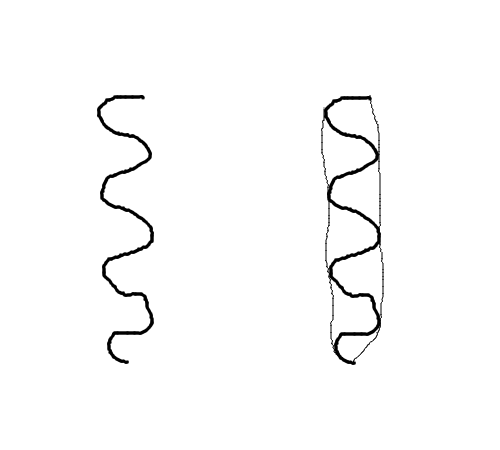
\includegraphics[keepaspectratio,width=400pt,height=0.75\textheight]{4_convex_freespace1.png}
\caption{Free space data before and after convex hull.}
\label{convex_free1}
\end{figure}



\begin{figure}[htbp]
\centering
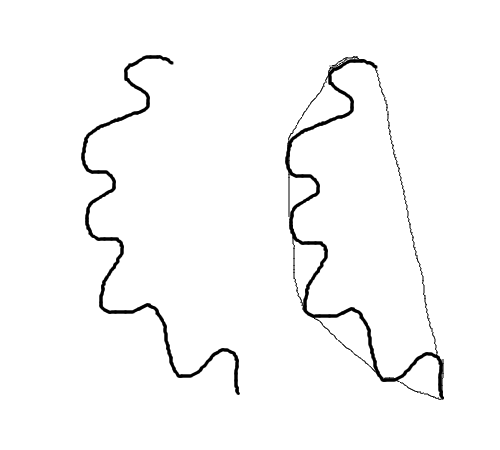
\includegraphics[keepaspectratio,width=400pt,height=0.75\textheight]{4_convex_freespace2.png}
\caption{Free space data of curved posture before and after convex hull.}
\label{convex_free2}
\end{figure}




An example of the convex hull operation on our free space data set appears in \autoref{convex_free1}. We can see for the case that the snake is in a straight pipe, the convex hull creates a natural representation of the local pipe environment, filling in the blanks of our blind spot. However, if the pipe is curved as in \autoref{convex_free2}, the convex property of the polygon necessarily erases any concave properties of the environment. This also removes any sharp features of the environment such as corners. Therefore, any use we may have for the convex hull will be in limited situations.


%A common algorithm from computational geometry that finds a minimum convex polygon that fits all the points.  The points in our case are the grids that are marked with free space.   Convert theses pixesl to points at their centers, and we have input for a convex polygon.  The results look like 0.  Cite \cite{cgal:hs-chep2-12b}

%This has the capability of smoothing over the gaps from the blind spots.  Has shortcomings.  Loses corners.

%Has some uses, but for curved pipes, we lose critical information about the true pipe dimensions and their curved topology.  Does not represent nonconvex features.


\subsection{Alpha Shape}
\label{alphashape}

An alternative to the convex hull is the alpha shape \textbackslash{}cite\{Edelsbrunner:1983p772\}. Like the convex hull, it creates a polygon or polygons that contain all the points. Unlike the convex hull, it can construct a containing polygon with concave or even hole features. 

\begin{figure}[htbp]
\centering
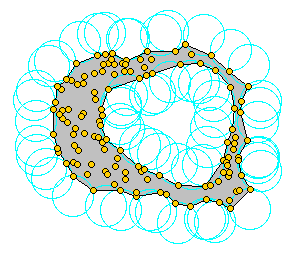
\includegraphics[keepaspectratio,width=400pt,height=0.75\textheight]{alphashape.png}
\caption{Alpha Shape example from \textbackslash{}cite[cgal:d-as2--12b]}
\label{alpha_cgal}
\end{figure}



To construct the alpha shape, first we choose a radius $r$ for a circle $C$. Next, if a pair of points $p_i$ and $p_j$ can be put on the boundary of $C$ where no other point is on or contained by $C$, we add an edge between $p_i$ and $p_j$. The result is seen in \autoref{alpha_cgal}

\begin{figure}[htbp]
\centering
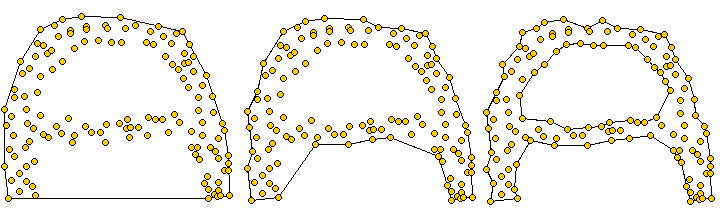
\includegraphics[keepaspectratio,width=400pt,height=0.75\textheight]{4_alpha_radius.png}
\caption{Alpha Shape changing radius from \textbackslash{}cite(cgal:d-as2--12b)}
\label{alpha_cgal2}
\end{figure}



By changing the radius size, we can tune how much smoothing we want to occur in the resultant polygon, seen in \autoref{alpha_cgal2}. If we set the radius to $r = \infty$, the alpha shape reduces to the convex hull. Therefore, this is a kind of ``generalized convex hull'' algorithm.

\begin{figure}[htbp]
\centering
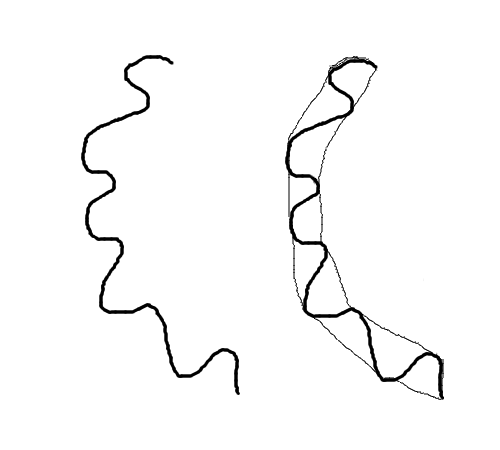
\includegraphics[keepaspectratio,width=400pt,height=0.75\textheight]{4_alpha_freespace2.png}
\caption{Alpha hull of free space data.}
\label{alpha_free2}
\end{figure}



The benefit to this approach is that we can now capture the concave features of some of our local maps where the convex hull failed. Where \autoref{convex_free2} shows the convex hull, \autoref{alpha_free2} shows its corresponding alpha shape. In both cases, the blind spot it smoothed over and filled in. This approach still suffers from the loss of sharp salient corner features, but the gross topology of the local environment has been captured.

For clarity, we refer to the alpha shape of our local free space as the \emph{alpha hull} from here on out.

\subsection{Medial Axis}
\label{medialaxis}

Although polygons that represent the sweeped free space are useful, we need something that is more compact that also filters out the smoothing effects of blind spots and sharp features. That is, we want an approach where the negative effects of missing data, erroneous data, and loss of salient features are minimized.

For this purpose, we compute the medial axis, also sometimes known as thinning or skeletonization [cite]. This concept takes a shape and reduces it to a path or series of edges that follow the ``spine'' of a shape. Approaches range from a strict computational geometry approach such as the Voronoi diagram to image processing approaches of image thinning and skeletonization that erode a pixelized shape until the skeleton is all that remains [cite].


%Skeletonization of a binary image.
%Black values (0) mean object and white values (1 = 255) background.
%Source: Parker, J.R. Algorithms for image processing and computer vision.
%               New York, NY: John Wiley & Sons, 1997. 417p. pp. 203-218.
%
%Program adapted to C/OpenCV by Jose Iguelmar Miranda.
%March, 2010.
%I have also a Java version of this program.


\begin{figure}[htbp]
\centering
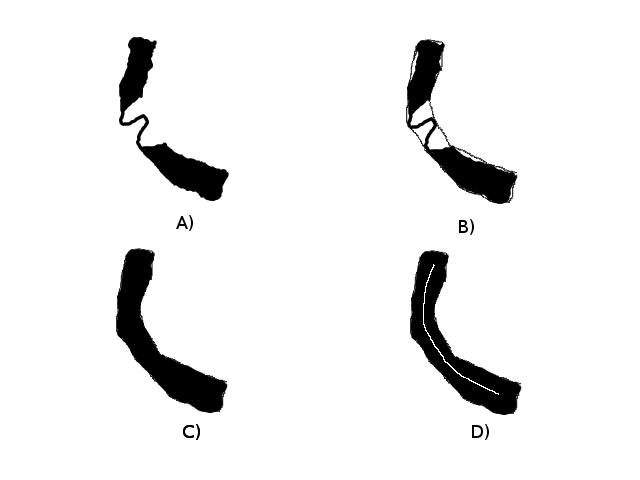
\includegraphics[keepaspectratio,width=400pt,height=0.75\textheight]{4_medial_process.png}
\caption{Process of generating medial axis.}
\label{medial1}
\end{figure}



\begin{figure}[htbp]
\centering
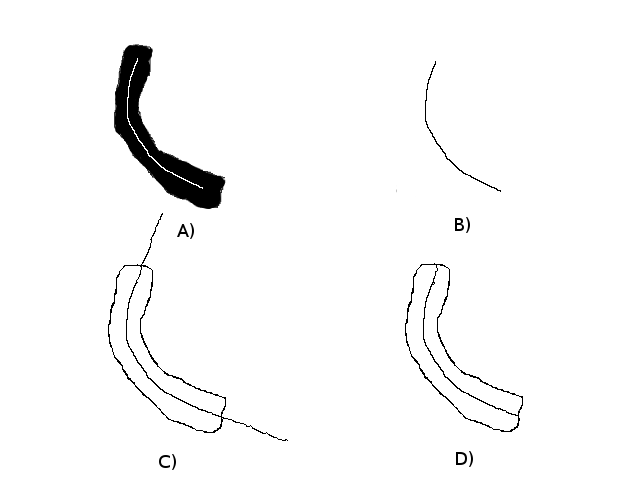
\includegraphics[keepaspectratio,width=400pt,height=0.75\textheight]{4_medial_process2.png}
\caption{Process of generating medial axis.}
\label{medial2}
\end{figure}




We are interested in extracting the medial axis of the alpha hull generated from our free space map. Since the alpha hull smooths the boundaries of the free space map, generating a medial axis will give us a topological representation of the free space that is resistant to boundary features. Given the free space map in \autoref{medial1}a, and its corresponding alpha hull in \autoref{medial1}b, the alpha hull's conversion back to an image in \autoref{medial1}c, and its resultant medial axis shown in \autoref{medial1}d. We use the skeletonization algorithm from [ParkerJR] \textbackslash{}footnote\{C\slash OpenCV code written by Jose Iguelmar Miranda, 2010\}.

sWe can see that the medial axis roughly corresponds to the topological representation of the pipe environment. However, it is crooked, pixelated, and does not extend the full length of the data set. We further treat this data to give a more useful representatation.

Starting with the result from \autoref{medial1}d shown in \autoref{medial2}a, we create a minimum spanning tree (MST) graph where each node is a pixel from the medial axis and an edge is added between two nodes if their corresponding pixels are neighbors, shown in \autoref{medial2}b.

This MST has many leafs due to the artifacts of pixelation. We can simply prune the whole tree by sorting all nodes by degree, and removing the nodes with 1 degree and their corresponding edges. In most cases, this will leave us with a single ordered path of nodes with no branches. In some cases, we will have a branch if the original free space map shows evidence of a junction.

In the case of a single path, our next step is to extend this path to full extent of the original shape. We begin by fitting a B-Spline curve to the ordered path. With an appropriate smoothing parameter, the spline curve will follow the path of the ordered points but will ignore the jagged edges from pixelation. We then uniformly sample points along this curve to convert it back to an ordered set of points. We extend this path in the front and back by extrapolating more points along the direction specified by the curve tip, as in \autoref{medial2}c. Multiple tangent vectors are sampled along the tip neighborhood and their direction is averaged to get a direction that is immune to spline curving artifacts at the terminals. Finally, the series of points is cut off once the extrapolated points cross the alpha hull boundary, shown in \autoref{medial2}d.

In the case that we have a branch, we perform this series of operations for the path between each combination of pairs of terminals. For each medial axis of a free space map, there are $n = 2 + B$ end points where $B$ is the number of branches. The number of unique paths of a medial axis is found by ${n \choose 2}$ since we are using the MST and there is a unique path between each pair of points.

The final form is a compact representation of the topology of the local free space that removes the noise and uncertainty of the boundary and allows us to only represent the area we can move through. This has a number of uses for our map-making that we describe in the next chapter. 


% environment -> free space map -> alpha hull -> image of alpha hull interior -> medial axis -> graph -> MST -> Spline -> sampled points -> extrapolation -> cutoff at boundary -> overlap of environment 


\section{Managing Slip}
\label{managingslip}

Since the possibility of error occurring in our free space maps is very real and has the consequences of making the data near-useless, we want to do all we can to prevent and mitigate any failure conditions. As the primary source of error is anchor slip, we do all we can to focus on this issue while probing the environment. We use a number of techniques for both prevention and detection of error. We describe all of our approaches below.

\subsection{Slip Prevention}
\label{slipprevention}

We have 6 strategies for preventing anchor slip during the course of probing the environment. These are the following:


\begin{enumerate} \itemsep 1pt \parskip 0pt \parsep 0pt
  \item Prescriptive Stability
  \item Local Stability
  \item Smooth Motion
  \item Averaging Reference Poses
  \item Separation of Sweep Maps
\end{enumerate}


The first three we have discussed earlier, with prescriptive stability and local stability in section \autoref{sec:anchors} and smooth motion in section \autoref{sec:smooth}. We use prescriptive and local stability to determine which reference poses are available to be activated. Whereas, smooth motion through the use of linearly interpolated steps by using the Transition behavior reduces the chance that our anchors will slip. 

The prescriptive stability selection of the PokeWalls behavior requires the robot to only use the anchored portion of the snake body for reference poses. In particular, it is very conservative, where only the segments at the very back and mechanically isolated from any of the sweeping motions in the front will be used for reference. This reduces the chance that any perturbations from the probing motions will have an effect on any of the active reference poses that we are using.

\subsubsection{Averaging Reference Poses}
\label{averagingreferenceposes}

For our fourth strategy, when actually using the reference poses to compute the position of the snake in our local free space map, we want to use as many of the reference poses as possible while filtering out any errors that would occur from possible pathological cases. If just one reference pose is erroneous and we use that reference pose to compute position of the snake in free space, it will severely damage our results. We want to mitigate the possibility of negative effects by taking the average of a set of reference poses when computing a snake's position.

For instance, if we wanted to compute the origin of our local free space map in global space, we would compute the kinematic position of joint 19 with respect to some active reference pose $P_k$ on joint and segment $k$. Using equation \autoref{kinem1} or \autoref{kinem2}, we compute the position of $P^{k}_{19}$. For every $P_k$ we use, we compute a new $P^{k}_{19}$ that is possibly different. We then take the average of all of the computed $P^{k}_{19}$ poses and take that as our best guess for $P_{19}$. 

\begin{figure}[htbp]
\centering
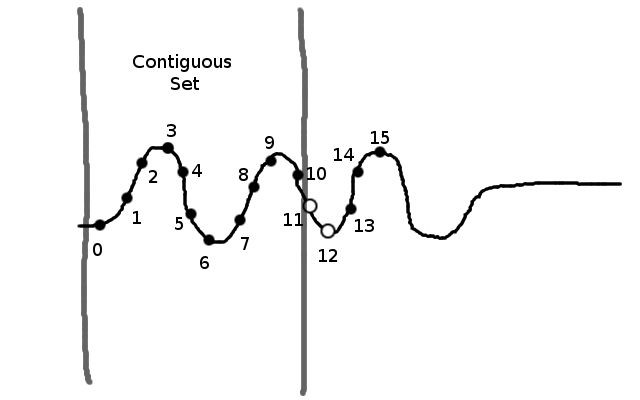
\includegraphics[keepaspectratio,width=400pt,height=0.75\textheight]{4_ref_averaging.png}
\caption{Largest set of contiguous reference poses.}
\label{ref_average}
\end{figure}



How do we select the set of active reference poses from which to compute our estimated snake pose? Of all available active reference poses, our approach is to use the largest set of contiguous poses to compute the average target pose $P_{19}$. Our assumption is that if we have a series of reference poses from 0 to 15, and 11 and 12 are deactivated, it is highly possible that 13, 14, and 15 are invalid because whatever caused 11 and 12 to be activated will likely have an effect on its neighbors. The larger section from 0 to 9 has less likelihood of being corrupted since more of our sensors indicate stability. Furthermore, if one or two of these reference poses are corrupted, having a larger set reduces the weight of an erroneous value. This example is shown in \autoref{ref_average}.

\subsubsection{Separation of Sweep Maps}
\label{separationofsweepmaps}

Our fifth and final strategy for preventing errors in our sensor maps is to divide the forward sweep phase and backward sweep phase into separate maps. From our experiments, we determined that a consistent source of error occurs when switching the anchoring responsibility from the back half of the snake to the front half. The series of events of retracting the front half of the snake to anchors and extending the back half for sweeping tends to cause some discontinuity between the consensus of the back reference poses and the front reference poses. This will show with a very distinct break in the combined free space map.

\begin{figure}[htbp]
\centering
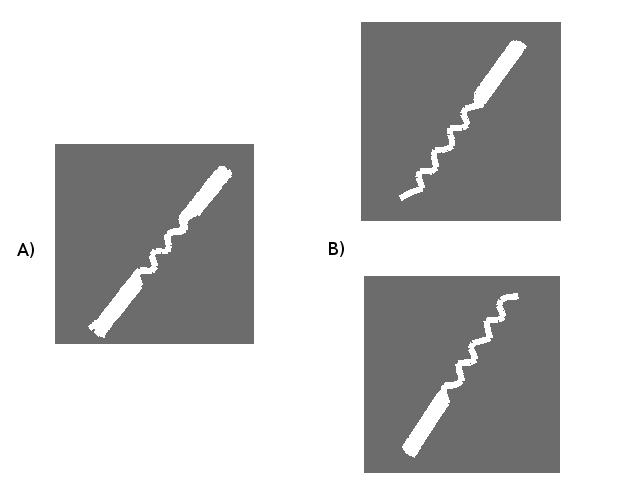
\includegraphics[keepaspectratio,width=400pt,height=0.75\textheight]{4_sweepmap_1.png}
\caption{Separation of Sweep Maps.}
\label{ref_sweep_sep}
\end{figure}



To avoid this problem, we instead create two free space maps: one for the front sweep and one for the back sweep. What was previously shown in \autoref{ref_sweep_sep}a will now become the pair of maps shown in Figure b. Not only does this avoid corrupting the free space data in the map, but it allows us to treat the relationship between the two maps as a separate problem for which there are multiple solutions. Our previous sensor processing algorithms work just as well because the alpha shape of the half-sweep free space map will result in an alpha hull from which an equivalent medial axis can be extracted. 

We discuss our approach to managing the relationship between the two half-sweep local maps in the next chapter.


%The fourth strategy is in regard to how to use the reference poses to compute the pose of a robot segment in space.  Instead of selecting one reference pose to use and hoping that it is 100 percent correct, we take a set of reference poses and average the computed position of a target segment.  How we select the set of references to use is by looking for the largest contiguous set.  That is, reference poses that are active and are all neighbors, we select the largest set.  If for instance, a set of 15 reference poses are used in time \\(t\\) and later reference pose 10 becomes deactived, for time \\(t+1\\), we assume that the poses \\(0-9\\) are still immobile and not \\(11-15\\).  Our heuristic assumes that it is much easier to move less segments than more.  



%-- averaged position from the back anchor reference poses
%-- only use backy-back reference poses to minimize possibility of bad reference poses being used.   Prescriptive stability is very conservative.
% Separation of forward sweep and backward sweep local maps.  Do not merge them but keep them separate and correctable.
% Error comes from the switch in posture from back-anchor/forward sweep to front-anchor/backward sweep


\subsection{Slip Mitigation}
\label{slipmitigation}

In the case that error is introduced into our local free space map, we are interested in mitigating its negative effects. We have developed two approaches for handling error when it occurs during sensing.

Since we start our mapping process by determining the global pose of the local origin $P_{19}$, error occurs when $P_{19}$ is no longer in its proper place. Either it moves by translation or more commonly and critically, it experiences rotational error. 

\subsubsection{Reference Stabilization}
\label{sec:ref_stable}

\begin{figure}[htbp]
\centering
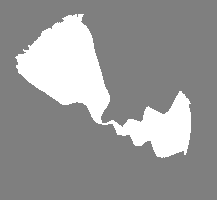
\includegraphics[keepaspectratio,width=400pt,height=0.75\textheight]{localMapError.png}
\caption{Local map rotational error.}
\label{ref_rot_error}
\end{figure}


A sudden rotation of $P_{19}$ may occur, caused by any of the reasons detailed in Section \autoref{sec:anchors}. The consequences of rotational error is that the entire body of the snake will rotate around the origin within the local map. This will result in a map feature shown in \autoref{ref_rot_error}.

We proactively combat this possibility by running a reference stabilization algorithm that continually corrects the local origin $O_t$ for $P_{19}$ in the local map at time $t$. For $t=0$, the origin is $(0,0,0)$ for inputing into the equations \autoref{equ:rect1} and \autoref{equ:rect2}. However, for each time step, we wish to calculate an $O_t$ that is the most ``stable'' in case $P_{19}$ becomes destabilized.

To do this, we remark that during the probing phase, the back anchored section of the snake as a whole will remainly roughly in the same tight space even if its joints and ssegments should wobble and slip. Short a large amount of translational slipping down the pipe, taken as a whole, the body should remain in the same place. Therefore, in the local free space map, the back anchored portion should of the snapshot time $t$ should also remain in the same neighborhood of the back anchor snapshot at time $t-1$. 

\begin{figure}[htbp]
\centering
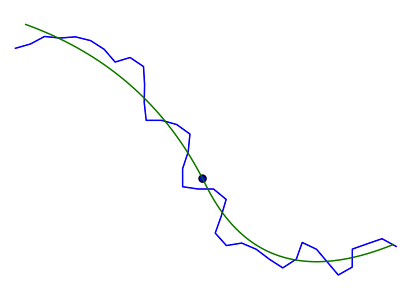
\includegraphics[keepaspectratio,width=400pt,height=0.75\textheight]{plotGPAC0059.png}
\caption{Gross Posture Approximation Curve of sample posture.}
\label{ref_gpac}
\end{figure}



We enforce this observation by fitting B-spline curve $\beta_t$ and $\beta_{t+1}$ along the points that make up the reference poses of the back anchor segments for both the current and previous snapshots. The B-spline curves are calibrated to smooth out the sinusoidal anchoring posture of the snake body and instead reflect the gross posture of the body in the confined environment as shown in \autoref{ref_gpac}. We then find a $(\delta x, \delta y, \delta \theta)$ for $\beta_{t+1}$ such that the two curves are aligned and then we update $O_{t+1}$ to reflect this.

This approach prevents sudden rotational errors from occurring and corrects the snake's estimated pose in the local map while we are capturing sensor data by generating a new $O_{t+1}$ that is consistent with past data. So even if the snake's body is wobbling or slipping, we will likely produce consistent sensor data.

Should the data be too hopelessly corrupted from a bow tie effect in the posture image, we can reject the overall data and take the instantaneous shot of the current posture as the only data. This gives a sparse snapshot of the environment and leaves the exploratory data out, but if will capture the gross shape of the local environments.


%Our goal is to detect when this first occurs and compensate to keep the map consistent.  We accomplish this by determining if the new posture snapshot suddenly jumps out of the local free space area we have already mapped.  The time between snapshots is very short and the snake probe is moving slowly enough that this is a reasonable assumption.

%We accomplish this by doing the following.   At every timestep \\(t\\), we have previously computed the alpha hull \\(H_{t-1}\\) for the current free space map.   For the current posture \\(\bar{\phi_t}\\), and for its position in the free space map using equations [](#equ:rect1) and [](#equ:rect2) and starting from the origin \\(O_{t-1}\\), determine if its position breaches the boundary of \\(H_{t-1}\\) by distance \\(d_h\\).

%--- we suppose that a significant rotational error has occurred.  In this case, we alter the location of the root pose from origin to an offset that keeps the posture inside the polygon boundary.  
%--- Correction is achieved by creating a spline of the back segments of the original and the current back posture.  The back splines are re-aligned and the pose of the root node is recomputed using this is a constraint.


\pagebreak 

\chapter{Environmental Landmarks}
\label{environmentallandmarks}

How to build features and landmarks from void space data? Need to build a map and localize against. Most feature techniques use boundary information as primitives for environmental features. Need approach that uses only void space.

Features to build the map

Boundary features
Obstacles\slash walls
Corners

Void space features
Shape features
Spatial features

\section{Finding Landmarks}
\label{findinglandmarks}

Seeking landmark features for which we can correct the map and localize the robot. Most approaches use point features such as corners, environmental landmarks such as doors, visual features. Our options are very limited because we do not have sensing at a distance capability. All things that we can sense must be within touching distance. Any feature we choose is highly local.

One option is to find corner features by probing the walls. There are two approaches: 1) deliberate contact probing of the wall to produce corner features, 2) serendipitous corner features. Problem: 1 is feasible but slow, see [Mazzini]. 2) is also possible but the false positive rate is too high. Pull some data out of my archives.

Also try and find “obstacles” and “openings” . That is, non-obstacle openings. This presupposes that we can distinguish obstacles. Only contact probing methods can truly classify an obstacle boundary. Again, these methods suffer from time-consuming actions. Furthermore, this does not exactly give us a true positive for open space. So door openings cannot be a landmark since we cannot detect them directly.

What about the walls of the environment? The shape of the obstacles? This requires that we fully mark the boundaries of walls and obstacles. Either this is done through laborious contact detection or we make assumptions about what are obstacles based on the data we receive serendipitously. Given a posture image, we could make varying degrees of assumptions about where the boundaries of the environment lie. None of them are likely to be correct, but we can use this information as a “feature”. However, this approach suffers when our probing actions are deficient for a particular pose. We receive a degenerate posture image that leaves out a lot of data. 

Another approach we could take is a sort of approximation and averaging of boundaries of the posture images. This can be accomplished by the use of the alpha shape algorithm developed in [3]. It is a form of generalized convex hull algorithm that is capable of non convex polygons. This can give us our desired “approximation” effect for identifying the location of walls.

\section{Corner Examples and Results}
\label{cornerexamplesandresults}

Corners are high false positive and too many false negatives.

Requires tuning of parameters, but does not guarantee correction selection.

Corners through serendipitous detection are not seen very often. Will not be seen through consecutive poses or even being in the same location. Not guaranteed to view.

Information too sparse to be useful. False correlation is very costly.

\section{Wall Detection}
\label{walldetection}

Contact detection literature. Reference 2009 paper.

Time spent probing walls. Amount of information is broken up. Example information should walls from contact detection.

Punch probing. Hit the wall and measure the error incurred by the joints in the control loop. Avoids the need for torque sensor. Uses existing control algorithm parameter as error terms.

Broken information, time-consuming. Error prone and often will mark free space as wall. Not detailed enough for a landmark feature.

\section{Different Macro Features}
\label{differentmacrofeatures}

The possibilities for curves representing the overall macro structure of the local environment are as follows:

\begin{enumerate}
\item Curves fitting through the anchor points of the articulated robot. Anchor points are the “confirmed” contacts and can approximate the walls. However, these are sparse data points, and cannot handle complex environments such as junctions or gaps between the anchor points. Data is sparse and not well-representative of the environment.

\item Polygon created from alpha shape of posture image. Use the edges of the polygon and perform scan-matching of edges to edges. Problem, how to select the points pairs between two polygons. Use angle filter and match two sides together. Is sensitive to missing data. Unsweeped gap will distort the polygon. Performing matches on a distorted polygon will result in poor ICP fitting.

\item Given alpha shape, compute the medial axis of the interior. This is known to be a reduction and representation of the the space. This approach is resistant to noisy edges. Shown are some example of the results with simple single path pipes, and pipes with some junction features. Notice that the information on the width of the environment is lost using this approach. 

\end{enumerate}

Shape of the sensed void space in local environment should give us information.
How can we extract this information and represent it in an useful way?

Spatial curve ct = scurve(It) where It is posture image
Smoothed version gives us a curve representation of the local space
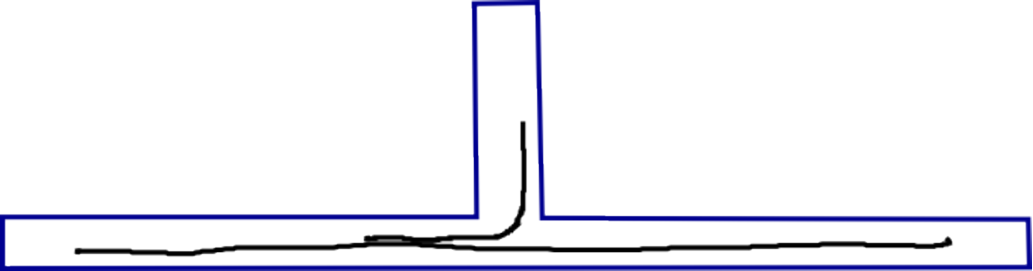
\includegraphics[keepaspectratio,width=\textwidth,height=0.75\textheight]{PastedGraphic.pdf}


\section{Macro Feature Extraction}
\label{macrofeatureextraction}

\begin{enumerate}
\item curve of anchor points, represents walls. Does not include sensed data

\end{enumerate}

Posture Image -$>$ Alpha Shape -$>$ Medial Axis -$>$ Characteristic Curve

Medial axis is generated from an image and a tree is built. I most cases the tree has only two leafs and is a “path graph”, but sometimes the tree has more than two leafs and represents more complex space.

Represents local description of space. 

Like scan-matching, we can use curves and ICP to find an alignment of the poses. The curves themselves becomes the landmarks.

\section{Pipe Shape, Macro Features}
\label{pipeshapemacrofeatures}

Use the contours and shape of the occupied space as our landmark feature. 

Introduces strong lateral correlation, but weak forward-backward correlation. If the local environment is curved in any way, this provides stronger localization.

\emph{1st order curve is straight line. Only coaxial localization between poses
}2nd order curve is a constant curve. Localization to any place with same curve constant.
*3rd order curve is changing curvature. Localization to unique point with particular change profile.s

3 different spatial features from posture images
blooms
arches
bends
Landmarks usually indicate junctions or gaps in space
Can match landmarks together to improve the map

\begin{figure}[htbp]
\centering
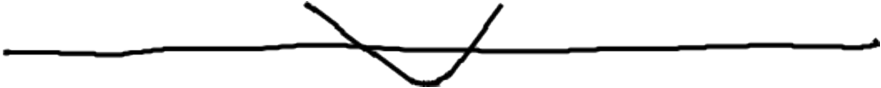
\includegraphics[keepaspectratio,width=\textwidth,height=0.75\textheight]{PastedGraphic1.pdf}
\label{pastedgraphic1.pdf}
\end{figure}



\begin{figure}[htbp]
\centering
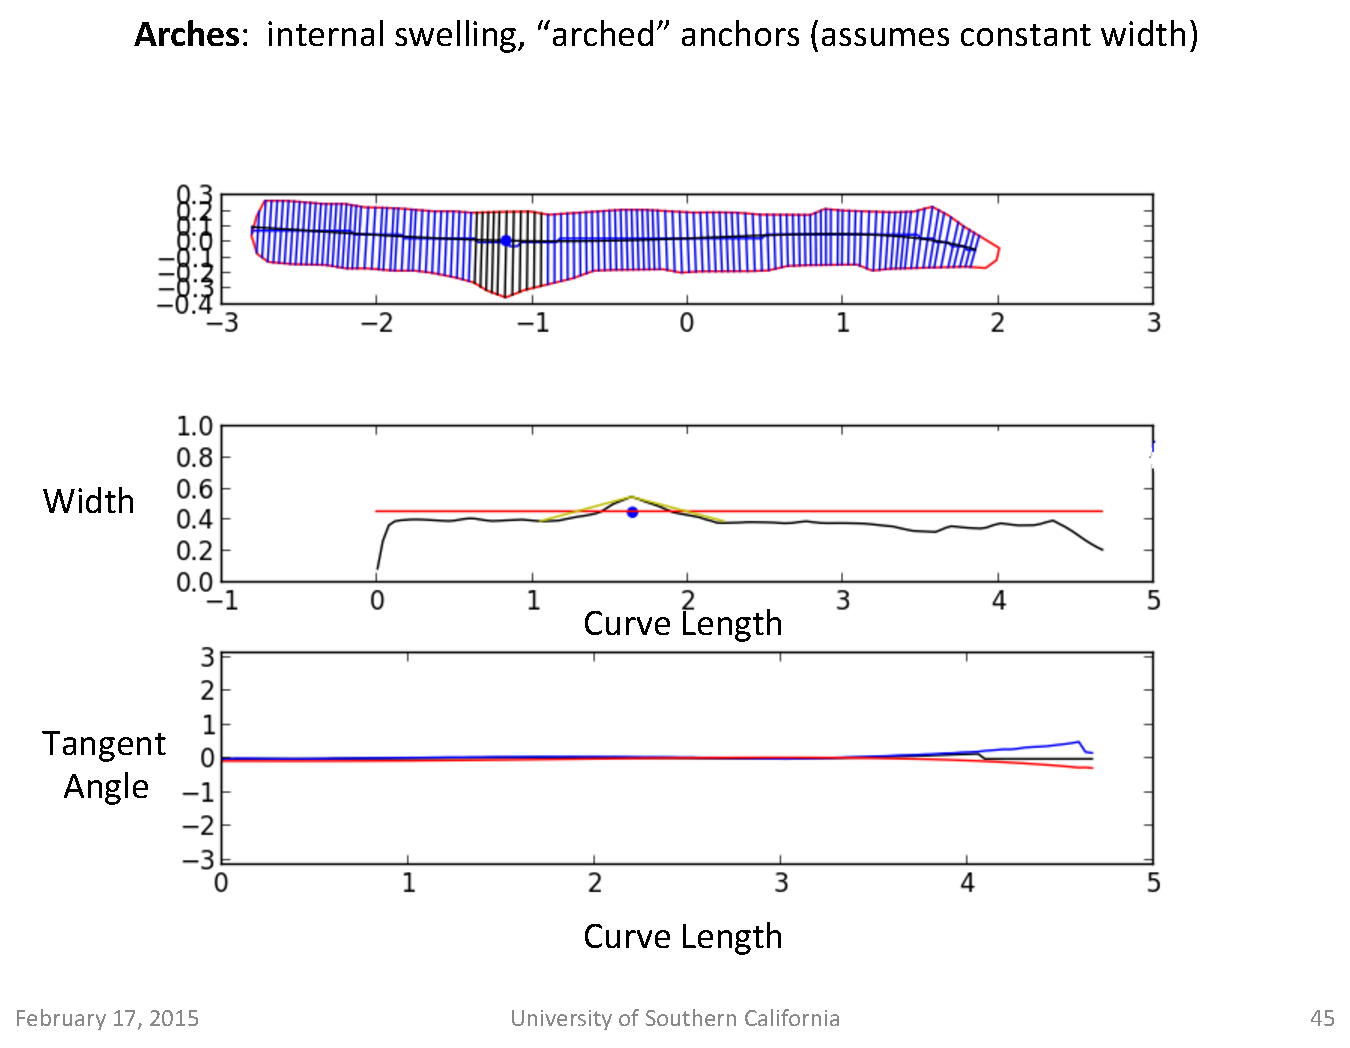
\includegraphics[keepaspectratio,width=\textwidth,height=0.75\textheight]{PastedGraphic2.pdf}
\label{pastedgraphic2.pdf}
\end{figure}




\begin{figure}[htbp]
\centering
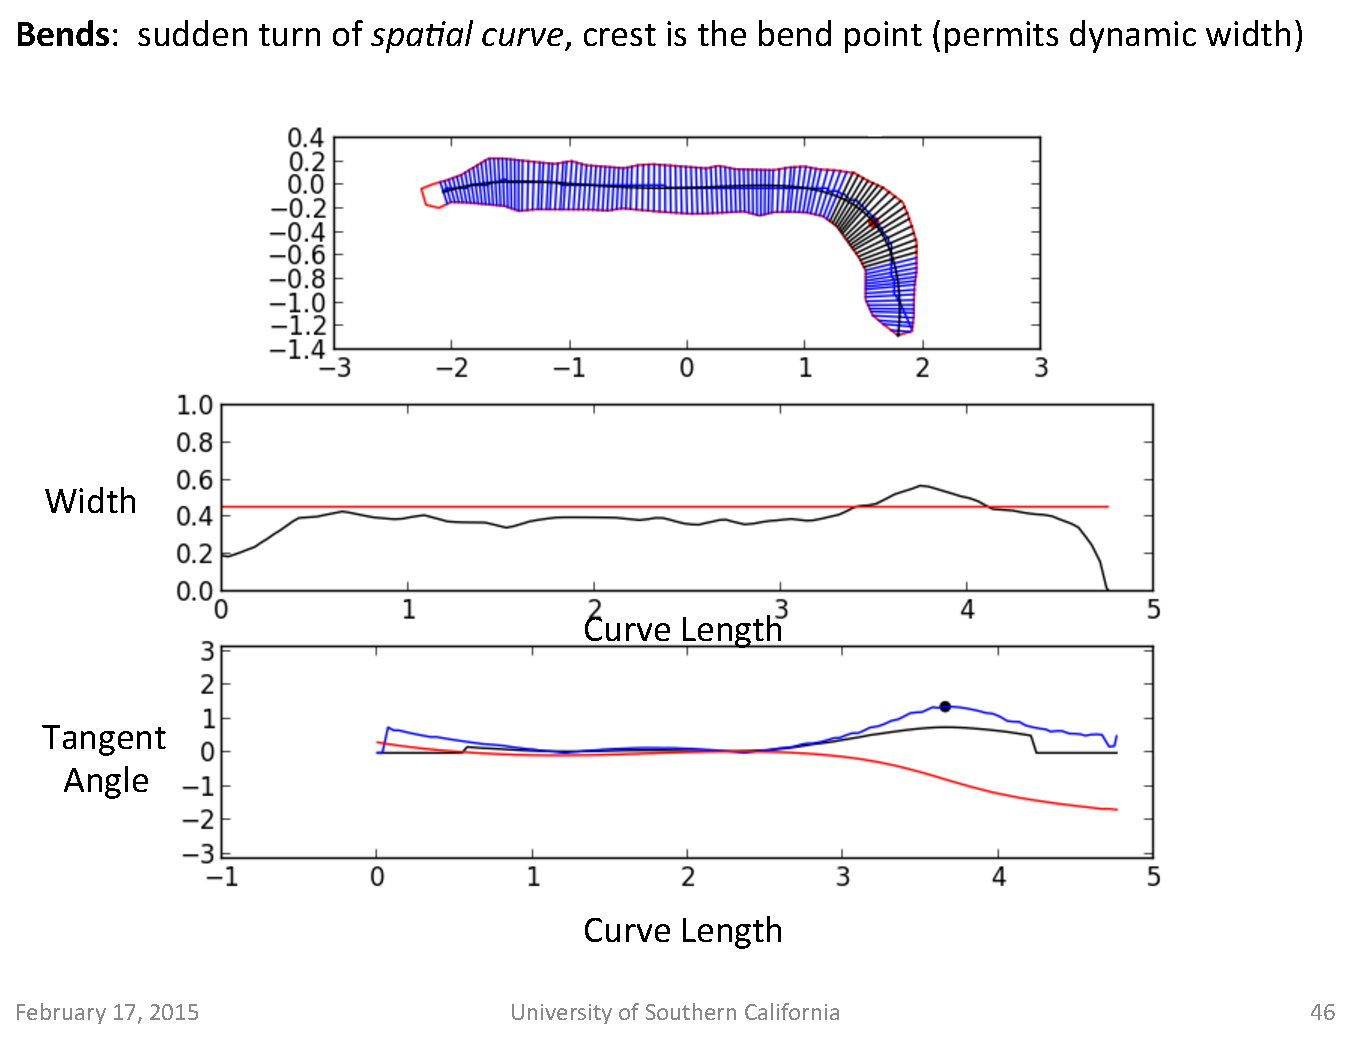
\includegraphics[keepaspectratio,width=\textwidth,height=0.75\textheight]{PastedGraphic3.pdf}
\label{pastedgraphic3.pdf}
\end{figure}





\pagebreak 

\chapter{Defining Position}
\label{definingposition}

\section{Problem}
\label{position:problem}

Now that our snake robot is capable of moving through the environment with the adaptive concertina gait behavior, we need some way of estimating how far it is moving and in which direction.

As we established earlier, we have no external sensors because we assume their failure from environmental conditions. We cannot rely on GPS since it is not effective underground or in pipes. We do not have wheeled shaft encoders since we have no wheels and do not expect to always travel through flat terrain. Finally, although it may indeed help, we cannot expect to make use of an inertial navigation system since they are bulky and expensive. Furthermore, we have not performed experiments to determine if they are capable of handling the high amount of rotation of each of the snake body segments during locomotion.

In absence of a global positioning or odometry, we need some form of alternative motion estimation. Knowing where the robot is located is the basic building block of creating a map. We focus on the problem of finding the relative geometric transform between the two poses at the beginning and end of one step of the adaptive concertina gait. 

But we first need to define how we will represent the position and orientation of the robot in space.

Our proprioceptive approach achieves motion estimation by anchoring multiple points of the body with the environment and kinematically tracking the change in distance between the immobilized parts as the snake contracts and extends. This gives us a motion estimation method that only depends on the joint sensors. We show the effectiveness in a series of experiments.

\section{Immobilizing the Anchors}
\label{sec:anchors}


%-Immobilize anchors to create global references
%-Conditions when immobility or anchor slip occurs
%-How to know when immobilized (heuristics)


A fundamental property of the adaptive concertina gait is that it creates anchors to the surrounding environment. Our goal is to exploit this property to estimate our motion through the environment. In order to do this, we need to ensure that our anchors remain an accurate frame of reference to the global environment.

The primary goal of our previous work on maintaining smooth and stable motion of the snake in Chapter 2 was to prevent any sort of anchor slip that may harm our reference frame to the global environment. It is critical that our anchors remain firmly immobilized with respect to the environment to ensure accurate measurement of motion.

Though we are not able to localize the exact contact point of the anchor with the environment, we can assume that the segments comprising the anchoring curve are themselves immobilized and mechanically isolated by virtue of their static contacts with the environment. We use these isolated bodies as immobilized references to the global environment.

Whether or not we consider the use of a body segment as a reference is determined by our work in Section 2.8. That is, if the joints in the local neighborhood of a segment are locally stable and the behavior's control bit for the attached joint is 0, we assume this segment is immobilized. We can use immobilized segments as reference points to the global frame.

We call the monitoring of local joint variances as local stability and the output of the control masks as prescriptive stability. Though a body segment may be locally stable, it does not mean it is immobile. If we also include prescriptive stability, the behavior's prediction of what joints should be moving and what should not, then we greatly decrease the chances that we will use a slipping anchor as a reference.

If any point the anchor should slip while, our assumption that a body segment is immobilized is violated and could lead to accumulated errors in our motion technique. Therefore, it is critical that we analyze and mitigate all the possible failure modes for anchoring.

We are generally able to classify the types of anchoring and reference errors we encounter during both static and locomotive anchoring. For each, we are forced to either avoid the condition from occurring or detect and correct it. We list the failure modes and explain our mitigation strategy for each.

The \emph{floating reference} occurs when a locally stable segment is made a reference, but it is not part of an anchor. This was particularly troublesome in our early implementations, but we are able to largely avoid this failure mode by having the behaviors explicitly classifying which joints are part of an anchor. The other possibility for a floating anchor would be if an anchoring behavior erroneously reports success in establishing an anchor in free space. This was largely avoided by adding the more careful anchoring process in Section 2.2 that detects impacts to the walls and follows up by doing a jerk test to test whether the anchor is secure.

A \emph{weak contact} occurs when the anchor the reference segment is on has an insecure anchor. This usually happens if an anchor is placed within a pipe junction or if one of the anchors of the Back-Anchor is insecure. The Back-Anchor case is more likely since they are not jerk-tested. Weak contacts usually do not display local instability since the physical contact stabilizes the local joints but does not immobilize them. If it is available, we can use negative prescriptive stability from the behavior to minimize this failure but often occurs in prescriptively stable areas. There is nothing we can do to prevent this error from being added to the pose estimation besides detecting it. Luckily, a weak contact does not move much. Its error is bounded.

\emph{Buckling} occurs when the anchored joints are frozen in a non-optimal position and external stresses put excessive torque on one or more joints that forces the anchor into a reconfigured position. This is similar to mechanical buckling of structural members under compression. In this case, it is for an articulated system attempting to hold a rigid pose. Buckling is easily detectable by tripping our local stability conditions and will quickly remove the references and reuse them once the joints have settled down. We have also reduced this occurrence by having our anchoring behaviors search for non-deforming anchors as a natural by-product of algorithm 2.

\emph{Impulses} occur when the snake robot experiences a sudden collision or a buckling has occurred somewhere else in the robot. Usually this is not a fatal error and the robot will quickly return to its stable pose. However it can trip up the variance calculations and deactivate all the references we have leaving us with none. Recovery is achieved by resurrecting the last best reference, and assuming it is in the same pose. We show how to do this in the next section.

\emph{Funnel anchoring} occurs when a secure anchor is established between a pair of walls that are monotonically increasing in width. If the anchor receives a force that pushes it towards the direction of increasing width, its anchor can become permanently loose. This is especially problematic in cases of irregular environments where there are many possibilities for this to occur in local conditions. We currently do not have a solution for this yet.

Finally there is a class of \emph{whole body slip} that is completely undetectable with only joint positions. That is, the whole body could be slipping through an environment such as a straight and featureless pipe without causing any joint variance at all. This would only occur if the ground was exceptionally slippery and able to use the robot's momentum to move it large distances or if the robot was on a slope and gravity was exerting a global force. We avoid this error by limiting the environments we explore. Other environments may require extra sensor instrumentation such as accelerometers to detect this failure mode.

Rotational error is the dominant form of error we encounter because, unlike a traditional robot with a stable frame of reference on its chassis, every reference point in the snake robot's body is constantly in rotational motion. Any form of disturbance of a reference node will manifest itself with a rotational error that will propagate through kinematic computations of new reference nodes. Translational error occurs primarily by anchor slip. Rotational error is easier to correct in our later localization process in Chapter 5.

\section{Tracking Motion}
\label{trackingmotion}


%-What a reference is
%-each active reference can be used to compute the pose of the snake at that given time
%-active references may disagree with each other
%-take current oldest active reference to compute current pose
%-How to create new references (kinematic computation)
%-When to deactivate references (violation of local/pre stability)
%-Loss of all references recovery


In order to track motion through the environment, we need to establish our mathematical framework for defining the relative position of things between the robot and the environment. We then define the concept of a \emph{reference pose} to track the position of the environment while the snake is in motion.

\subsection{Pose and Coordinate Frames}
\label{poseandcoordinateframes}

\begin{figure}[htbp]
\centering
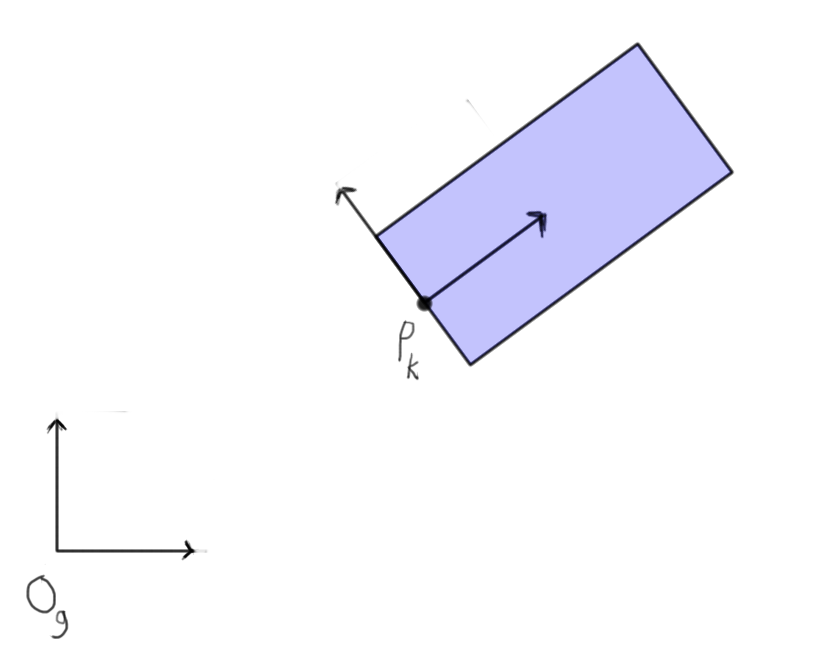
\includegraphics[keepaspectratio,width=400pt,height=0.75\textheight]{3_pose_frame1.png}
\caption{Pose of rigid body with respect to global frame.}
\label{fig:pose_frame1}
\end{figure}


A pose $P$ defines the position and orientation of a rigid body in a 2D plane. Each pose is defined with respect to a coordinate frame $O$ using 3 values: $(x,y,\theta)$. A coordinate frame is either affixed in the global environment or affixed to a rigid body on the snake. An example of the global frame $O_g$ and a pose $P_k$ are shown in \autoref{fig:pose_frame1}.

By convention, we will specify in the superscript which coordinate frame a pose $k$ is defined with respect to. For the global frame, the pose is written as $P_k^g$. If the pose is with respect to some other coordinate frame $O_a$, the pose is written as $P_k^a$. If the superscript is omitted, we assume the global frame.

\begin{figure}[htbp]
\centering
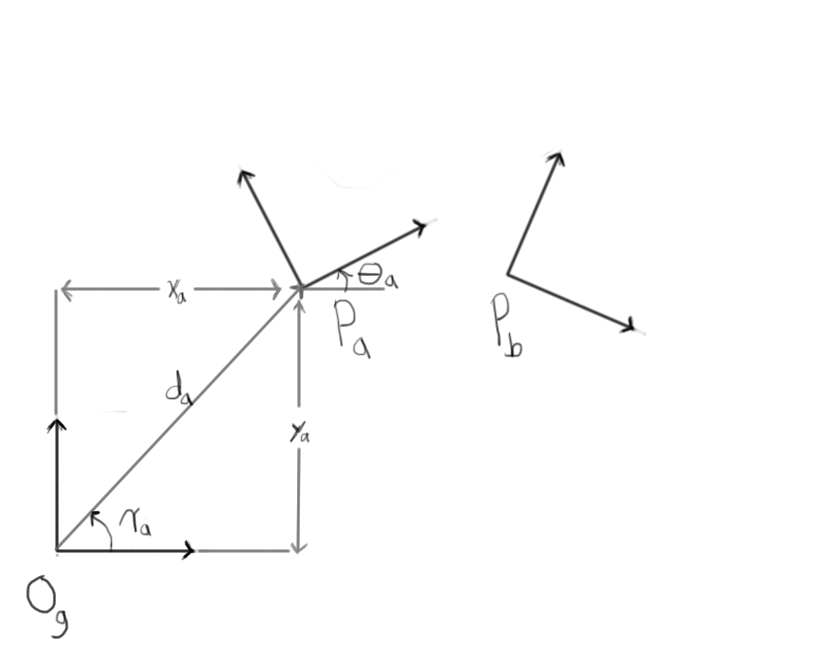
\includegraphics[keepaspectratio,width=400pt,height=0.75\textheight]{3_pose_frame2.png}
\caption{Pose of A and B with respect to global frame.}
\label{fig:pose_frame2}
\end{figure}



In a robot system with multiple rigid bodies, we will have a coordinate frame for each body. Often times, we wish to transform poses between coordinate frames. To do this, we first need to define the relationship between coordinate frames, specified by the pose of their origins. In the global frame $O_g$, the pose of the origin $O_g$ is $P_g = (0,0,0)$. For two example coordinate frames attached to rigid bodies, we define the pose of origin $O_a$ to be $P_a = (x_a, y_a, \theta_a)$ and the pose of origin $O_b$ to be $P_b = (x_b, y_b, \theta_b)$ as shown in \autoref{fig:pose_frame2}.

Suppose we wanted to compute pose $b$ with respect to frame $O_a$. That is, we wish to find $P_b^a$ and we are given $P_a^g$ and $P_b^g$. First we focus on finding the Cartesian component of the pose, point $p_b^a = (x_b^a, y_b^a)$. We compute the angle portion $\theta_b^a$ separately. From \autoref{fig:pose_frame2}, we define the following:


\begin{equation}
\label{equ:coord1}
R_a =
\begin{bmatrix}
cos(\theta_a) & sin(\theta_a) \\
-sin(\theta_a) & cos(\theta_a)
\end{bmatrix}
\end{equation}


This is the rotation matrix for the difference in orientation between the global frame $O_g$ and local frame $O_a$.


\begin{equation}
\label{equ:coord2}
d_a = \sqrt{(x_a)^2 + (y_a)^2} 
\end{equation}


This is the Cartesian distance from the global frame's origin to the local frame's origin.


\begin{equation}
\cos(\gamma_a) = \frac{(x_a,y_a) \cdot (1,0)}{|(x_a, y_a)| |1|} = \frac{x_a}{d_a} 
\end{equation}
\begin{equation}
\label{equ:coord3}
\gamma_a = s \cdot \arccos \left( \frac{x_a}{d_a} \right) 
\quad
\left\{ 
  \begin{array}{l l}
    s = 1 & \quad \text{if $y_a \geq 0$}\\
    s = -1 & \quad \text{if $y_a < 0$}
  \end{array} \right.
\end{equation}


$\gamma_a$ is the angle of the vector from the global origin to the local frame origin. The sign of $\gamma_a$ is determined to be negative if $y_a < 0$. Otherwise, $\gamma_a$ is positive. This value corresponds to the angle shown in \autoref{fig:pose_frame2}.


\begin{equation}
\label{equ:coord4}
G_a = 
\begin{bmatrix}
cos(\gamma_a) & sin(\gamma_a) \\
-sin(\gamma_a) & cos(\gamma_a)
\end{bmatrix}
\end{equation}


$G_a$ is the rotation matrix to rotate the local frame's origin onto the x-axis of the global frame.

To find $p_b^a$ in frame $O_a$ from $p_b^g$ in $O_g$, we compute:


\begin{equation}
\label{equ:g_to_c_cart}
p_b^a =
\begin{bmatrix}
x_b^a \\
y_b^a \\
\end{bmatrix}
 = R_a {G_a}^{\mathbf{T}} \left(G_a p_b^g 
-
\begin{bmatrix}
d_a \\
0
\end{bmatrix}
\right)
\end{equation}


To find the converse, $p_b^g$ from $p_b^a$, we do the following:


\begin{equation}
\label{equ:c_to_g_cart}
p_b^g =
\begin{bmatrix}
x_b^g \\
y_b^g \\
\end{bmatrix}
 = {G_a}^{\mathbf{T}} \left(
\begin{bmatrix}
d_a \\
0
\end{bmatrix}
+ G_a {R_a}^{\mathbf{T}} p_b^a \right)
\end{equation}


This approach performs a sequence of rotations to separate translation and rotation of the pose when converting between frames. To compute the angle portion of the pose, we perform the rotation sequence by addition and subtraction of angles. Following the sequence, we get the following: 


\begin{equation*}
\theta^a_b = \theta_b^g + \gamma_a - \gamma_a - \theta_a
\end{equation*}
This reduces to:
\begin{equation}
\label{equ:g_to_c_ori}
\theta^a_b = \theta_b^g - \theta_a
\end{equation}


The converse is achieved similarly using Equation \autoref{equ:c_to_g_cart} and the following rotation sequence:


\begin{equation*}
\theta_b^g = \theta_b^a + \theta_a + \gamma_a - \gamma_a 
\end{equation*}
\begin{equation}
\label{equ:c_to_g_ori}
\theta_b^g = \theta_b^a + \theta_a
\end{equation}


The final result for the pose computation is to put the Cartesian and angular components together.


\begin{equation}
P_b^a =
\begin{bmatrix}
x_b^a \\
y_b^a \\
\theta_b^a 
\end{bmatrix}
\quad
\left\{ 
  \begin{array}{l l}
    x_b^a,y_b^a & \quad \text{from Equation \ref{equ:g_to_c_cart}}\\
    \theta_b^a & \quad \text{from Equation \ref{equ:g_to_c_ori}}
  \end{array} \right.
\end{equation}


And the converse is:


\begin{equation}
P_b^g =
\begin{bmatrix}
x_b^g \\
y_b^g \\
\theta_b^g 
\end{bmatrix}
\quad
\left\{ 
  \begin{array}{l l}
    x_b^g,y_b^g & \quad \text{from Equation \ref{equ:c_to_g_cart}}\\
    \theta_b^g & \quad \text{from Equation \ref{equ:c_to_g_ori}}
  \end{array} \right.
\end{equation}


Now that we have established the mathematical framework for relating the pose of the rigid bodies to the environment and each other, we describe our concept of reference poses to track motion in the environment.

\subsection{Reference Poses}
\label{referenceposes}

A reference pose is the position and orientation of a rigid body segment that has been immobilized with respect to the global frame. A reference pose is valuable because it gives a fixed reference point to the global environment and allows us to track the motion of the rest of the robot. Special care must be taken to ensure that when using a reference pose, the rigid body it's attached to is truly immobilized.

A reference pose is either active or inactive. A reference is active once it is created as a result of its rigid body becoming immobilized. We assess whether a reference pose is to be created by checking if it satisfies both our predictive stability and local stability conditions. We discussed predictive and local stability in section \autoref{sec:stability}, where predictive stability is the output of the behavior's control masks and local stability is the result of monitoring local joint variances. Once the reference pose violates either of these conditions, it becomes inactive.

To deactivate a reference pose, if a reference violates either of the stability conditions and it was previously active, we flip a bit to signal it as inactive. Afterwards, we can create a new reference pose on this rigid body once it satisfies the stability conditions again.

To create a new reference pose, its associated rigid body must first have been inactive. Secondly, it must satisfy both prescriptive and local stability conditions. Once the following conditions have been met, the new pose is computed kinematically with respect to another currently active reference pose. If the pre-existing reference pose is correct, the kinematic computation of the new reference pose will be correct for its true position and orientation in the global environment.

Given the arrangement of rigid bodies and their attached coordinate frames shown in \autoref{frames2}, we need the kinematic equations for computing the pose of a rigid body given its neighbor's pose. That is, if we already have an active reference pose, we wish to compute the pose of neighboring reference in the global frame using only the joint angles from the robot's posture. To compute $P_{k+1}$ if we are given $P_k$, we do the following:


\begin{equation}
\begin{array}{l}
\displaystyle x_{k+1} = x_k + l \cos(\theta_k) \\
\displaystyle y_{k+1} = y_k + l \sin(\theta_k) \\
\displaystyle \theta_{k+1} = \theta_k - \phi_{k+1}
\end{array}
\label{kinem1}
\end{equation}
For the opposite direction, to compute $P_{k+1}$ given $P_k$, we do the following:
\begin{equation}
\begin{array}{l}
\displaystyle \theta_k = \theta_{k+1} + \phi_k \\
\displaystyle x_k = x_{k+1} - l \cos(\theta_k) \\ 
\displaystyle y_k = y_{k+1} - l \sin(\theta_k)
\end{array}
\label{kinem2}
\end{equation}


If we use the equations iteratively, we can compute the pose of a rigid body segment given the pose of any other segment. 

The algorithmic process for creating and deactivating reference poses is shown in Algorithm \autoref{alg:reference}, where $N$ is the number of rigid body segments in the snake from which to create reference poses. The implementation of the function for the kinematic computation of new reference poses is shown in Algorithm \autoref{alg:kinematic}.

\begin{figure}[htbp]
\centering
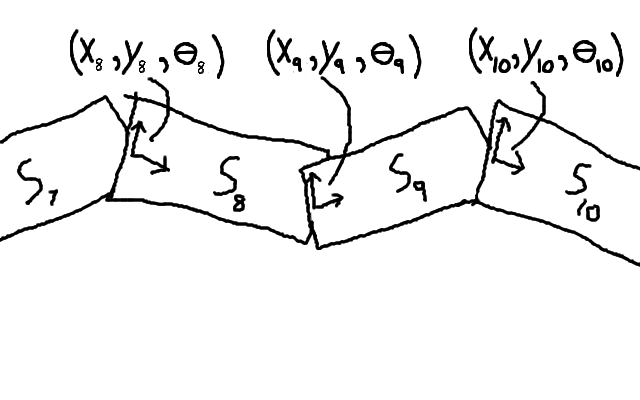
\includegraphics[keepaspectratio,width=400pt,height=0.75\textheight]{3_frames_2.png}
\caption{Local coordinate frames attached to segments and described by reference poses.}
\label{frames2}
\end{figure}




\begin{algorithm}
\caption{Reference Pose Creation and Deactivation}          % give the algorithm a caption
\label{alg:reference}
\begin{algorithmic}

\State $N \Leftarrow 40$
\State $activeMask \Leftarrow $ array of size $N$ initialized to $0$
\State $activeRefPoses \Leftarrow $ array of size $N$ initialized to $\varnothing$
\State $preStabMask \Leftarrow \mathrm{behaviorControlOutput}()$
\State $locStabMask \Leftarrow \mathrm{stabilityCompute()}$
\For{$i = 0 \to N$} 
\If  {$preStabMask[i] \And locStabMask[i]$}
\If    {$!activeMask[i]$}
\State      $activeRefPoses[i] \Leftarrow \mathrm{computeRefPose}(i)$
\State      $activeMask[i] \Leftarrow 1$
\EndIf
\ElsIf {$activeMask[i]$}
\State    $activeRefPoses[i] \Leftarrow \varnothing$
\State    $activeMask[i] \Leftarrow 0$
\EndIf
\EndFor

\end{algorithmic}
\end{algorithm}



\begin{algorithm}
\caption{\emph{computeRefPose(i)}: Kinematics for Computing Reference Pose}
\label{alg:kinematic}
\begin{algorithmic}

\State $N \Leftarrow 40$
\State $\bar{\phi} \Leftarrow $ array of current joint angles 
\State $i \Leftarrow $ target new reference pose index
\State $j \Leftarrow $ index of nearest active reference pose to $i$

\State $k = j$
\State $(x_k, y_k, \theta_k) \Leftarrow (x_j, y_j, \theta_j)$  \Comment{pose of active reference $j$}

\If {$i > j$}
\While {$k < i$}

\State $x_{k+1} = x_k + l \cos(\theta_k)$
\State $y_{k+1} = y_k + l \sin(\theta_k)$
\State $\theta_{k+1} = \theta_k - \phi_{k+1}$
\State $k = k + 1$
\EndWhile

\ElsIf {$i < j$}
\While {$k > i$}

\State $\theta_{k-1} = \theta_k + \phi_{k-1}$
\State $x_{k-1} = x_k - l \cos(\theta_{k-1})$
\State $y_{k-1} = y_k - l \sin(\theta_{k-1})$
\State $k = k - 1$

\EndWhile
\EndIf

\State $(x_i, y_i, \theta_i) \Leftarrow (x_k, y_k, \theta_k)$ \Comment{new pose for active reference $i$}

\end{algorithmic}
\end{algorithm}


This algorithm assumes that an active reference pose always exists. There are two special cases when no reference poses are currently active. In the first case, the algorithm is initializing and no reference poses have been created yet. In the second case, all of the reference poses violate the stability condition and all have been deactivated. These special cases are not shown in the algorithms, but we explain are approach here.

For the first case, when we initialize, the first reference pose is set to $(0,0,0)$. This becomes the origin of the global frame centered at the robot's starting position in the environment. From this first initial reference pose, all new reference poses are derived. 

In the second case, no active reference poses are available since no stability conditions have been satisfied. The robot has effectively lost track of its position in the environment. In the event that a new reference pose needs to be created, there is no parent pose from which to kinematically compute. Instead, from the last used inactive reference poses, we select the reference that was contiguously active the longest and use this as the parent pose to compute the new active reference pose. The reasoning behind this is that a long-lived reference pose is more likely to be correct than a short-lived reference pose due to the sometimes intermittent nature of reference poses. This last best reference pose approach is very effective in practice. 

So long as the active reference poses satisfy the assumption of no-slip anchors and there always being at least one active reference, the tracking of the robot's trajectory through the environment is correct. Violations of these assumptions introduce error into the motion estimation.

\section{Robot-Centered Coordinate Frame}
\label{sec:gpac}


%-N possible local coordinate systems in snake
%-none are very good to represent pose of snake because of the high variance in orientation.  Try to relate two poses to each other, orientation has almost no correlation
%-orientation is also primary source of error
%-prefer a coordinate system that represents the gross posture and pose of snake.  COM can sometimes be out of body
%-GPAC pose proposed.


Though we now have a local coordinate frame for each segment in the snake, we need a coordinate frame that represents the mobile robot body as a whole. In traditional mobile robots, we usually have a large rigid body chassis with high inertia that is suitable for defining the position and orientation of the robot. In a snake robot, there are multiple rigid bodies, all of which are small in mass, small in inertia, and poor at defining the overall snake's position and orientation. While the snake is executing its locomotion, the body segments are undulating and rapidly changing orientation, making dubious their use as an indication of heading.

In the wake of these phenomena, we found the need to create a dynamically generated coordinate frame that best represents the position and orientation of the snake robot's posture as a whole. We cannot use the center of mass of the robot, because the centroid can be outside of the body if the snake's posture is curved. Instead, we generate a curve called a Gross Posture Approximation Curve (GPAC) that we use to generate a local coordinate frame that is oriented in the direction of travel. This allows us to describe consecutive poses of the snake with local coordinate frames oriented in the same forward direction.

We describe in detail the GPAC and follow with the generation of the local coordinate frame.

Articulated robot has no high-inertia center of mass to serve as its coordinate frame. Require method to establish “forward” direction of an articulated robot.

Articulated robot has no high-inertia center of mass to serve as its coordinate frame.
Individual segments are rotating and undulating
Need method to determine direction of snake robot.
Information not provided by individual body segments
Posture curve generated by smoothed B-spline with joint locations as inputs
Generates the posture frame for local coordinate system
Different from spatial curve which represents local sensed environment 

Establishes stability of robot frame under error of anchoring.

\subsection{Gross Posture Approximation Curve (GPAC)}
\label{grosspostureapproximationcurvegpac}

The GPAC is a curve that approximates the posture of the robot in the environment without the articulation, as seen in \autoref{gpac}. The blue lines indicate the posture of the snake and the green line is the GPAC.

The GPAC is derived by taking the ordered points of the snake segment positions and fitting a smoothed B-spline curve to them. To generate the points, we first start from a body frame fixed to one of our body segments. In this case, we use segment 19 centered on joint 19 as our body frame $O_{19}$. With respect to frame $O_{19}$ and using the current joint posture vector $\hat{\phi_t}$, we compute the segment posture vector $\hat{\rho_t}$ that specifies the $N$ segment poses using the iterative kinematic equations \autoref{kinem1} and \autoref{kinem2}. If we take only the cartesian components of the segment posture $\bar{\rho_t}$, we set this as a series of ordered points from which we compute a B-spline curve.

\begin{figure}[htbp]
\centering
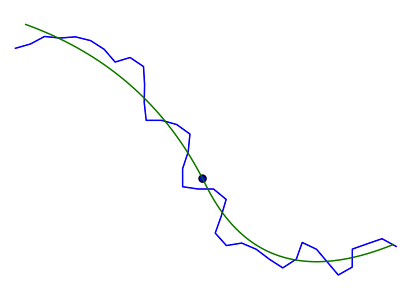
\includegraphics[keepaspectratio,width=400pt,height=0.75\textheight]{plotGPAC0059.png}
\caption{Robot Posture, Gross Posture Approximation Curve (GPAC), and Local Frame Origin}
\label{gpac}
\end{figure}



We use the Python SciPy library's \textbf{splprep} function with a smoothness factor of $0.5$ to generate the B-spline curve. This results in the curve shown in \autoref{gpac}. To use this curve, we define a set of parameterized functions that we use to access the curve. First we show the function provided by the SciPy library:


\begin{equation}
O(1): \quad \beta_t(u) = ( x_u, y_u, \theta_u ),  \quad 0 \leq u \leq 1
\end{equation}


This function gives us access to the curve with a normalized parameter $u$. The function returns the x and y coordinates of a point and the orientation of its tangent vector that correspond to the $u$ value. The drawback to this function is that the difference of arclength between two $\beta(u)$ values is not proportional to the difference in $u$ value. This implies that the following condition exists:


\begin{equation}
\mathbf{dist}(u_1, u_1 + K) \neq \mathbf{dist}(u_2, u_2 + K)  
\end{equation}


where the function $\mathbf{dist}()$ computes the arclength between two $u$ values on the curve, and the constant $K$ adds the same $u$ offset at two different points on the curve specified by $u_1$ and $u_2$. What this means in practical terms is, the $u$ values cannot be relied upon to give us reproducible positions on the curve. In particularly, if we retrieve the point $\beta_t(0.5)$, this will be close to the midpoint of the curve, but not the true midpoint and is subject to change between different curves.

We create a more accurate method that allows us to specify a point of true arclength on the curve. We present it in the form of a parameterized function:


\begin{equation}
\label{equ:arcdist}
O(\log n): \quad \sigma_t(d) = ( x_d, y_d, \theta_d ),  \quad 0 \leq d \leq d_{max}
\end{equation}


Here $d$ is the arclength starting from the $u = 0$ terminator of the curve. $d_{max}$ is the maximum arclength of the curve.

Though this is defined in the form of a function, it is implemented with a search algorithm. If we pre-process the curve by uniformly pre-sampling $n$ points with $\beta_t(u)$ in $O(n)$ time, we can achieve a binary search time of $O(\log n)$ for each invocation of the function. The $n$ parameter here corresponds to the number of samples of the curve we use to search over. The more samples, the more accurate the function will be. Here we use a tractable size of $n = 100$.

To perform the inverse operation for curve functions, we use the same pre-processed $n$ sample points from equation \autoref{equ:arcdist} and define the following functions:


\begin{equation}
O(n): \quad \beta^{-1}_t(x, y) = u
\end{equation}
\begin{equation}
O(n): \quad \sigma^{-1}_t(x, y) = d
\end{equation}


These inverse operators find the closest sample point on the curve to $(x,y)$ and returns the sample's associated $u$ or $d$ parameter. The correctness of these functions depend on the queried point being reasonably close to the curve, the curve not be self-intersecting, and the point not be equidistant to two disparate points on the curve. They are $O(n)$ because we must compute the distance to all $n$ sample points. Notice that we omit the angle portion of the curve for inverse operations. We do not define closest point for orientations.

Since these inverse curve functions are very similar, we develop a unified algorithm that produces parallel results. We do this to prevent duplication of search operations when similar information is needed.


\begin{equation}
O(n): \quad c_p(x,y) = (u, d, (x_p, y_p, \theta_p) )
\end{equation}


This function returns the closest point on the curve to $(x,y)$, and its associated $u$ and $d$ parameters.

Finally, we have functions that convert between $u$ and $d$.


\begin{equation}
O(\log n): \quad \mathbf{d}(u) = d
\end{equation}



\begin{equation}
O(\log n): \quad \mathbf{u}(d) = u
\end{equation}


These can be performed with a binary search on the pre-processed sample points.

\subsection{Generation of GPAC Local Frame}
\label{generationofgpaclocalframe}


%This produces a curve that approximates the general posture of the robot.  The middle point is selected by finding the location that is equidistant to the tips.  The tangent vector is used to orient the local coordinate frame.  This vector has the benefit of always pointing in the direction the robot is facing.

%and choose a point on the curve to act as our local coordinate system's origin.  This is seen in [](#GPAC).  Notice that the direction of the curve at the origin is in the forward-backward direction making this useful as a heading reference.


For each generation of the GPAC, we can create a unique but predictable coordinate frame that represents the gross posture of the snake in the environment. Because the GPAC only follows the general posture of the snake, regardless of its articulation, the difference in curves between generations is small and within reason.

Once we have the new GPAC, to determine the location of our new coordinate frame origin $\hat{O_t}$ with respect to $O_{19}$, we compute the following:


\begin{equation}
P_d = \sigma_t(d_{max} / 2)
\end{equation}


This specifies the halfway point along the curve in terms of arclength with respect to $O_t$. If we had used $\beta_t(0.5)$ instead, we would have had no guarantee how close to the middle it would be and no guarantees on repeatibility. By using the arclength function $\sigma_k()$, we have more guarantee over the location at the expense of running time.

From our new local frame $\hat{O_t}$, the orientation of the x-axis is directed in the forward direction of the snake, regardless of the articulation of the joints. This approach now gives us the tools to make relations between snake poses where the orientations will have some correlation. If we had insisted on using a body frame $O_{19}$ as a local coordinate frame, the orientations would have had very little correlation. We would have had no means to relate and correct orientations between snake poses.

In the future, we will drop the $t$ subscript of a GPAC and local frame origin and only refer to them as $\beta_k(u)$, $\hat{O}_k$, and $\hat{P}_k$, where $\hat{O}_k$ is the GPAC generated origin, $\hat{P}_k$ is the origin's location in the global frame, and $k$ is the particular pose number in the pose graph. We describe this in more detail in Section 5.

\begin{figure}[htbp]
\centering
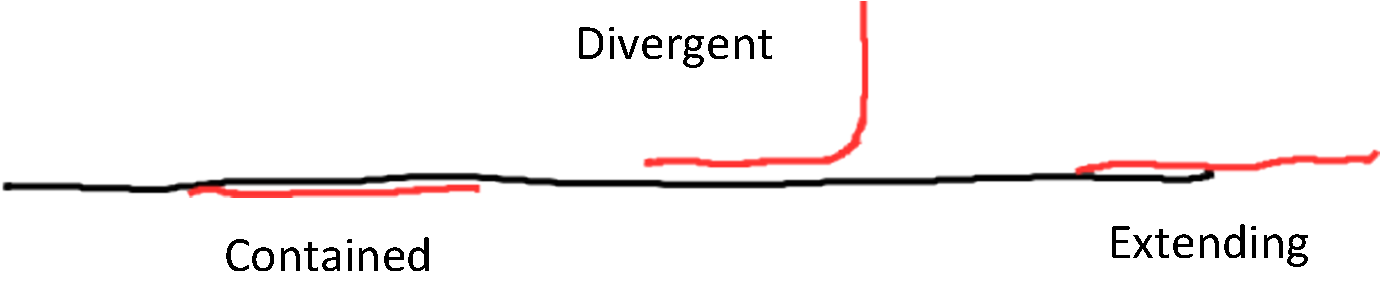
\includegraphics[keepaspectratio,width=\textwidth,height=0.75\textheight]{PastedGraphic4.pdf}
\label{pastedgraphic4.pdf}
\end{figure}



\subsection{Geometric Transform between Poses}
\label{sec:geo_transform}

Now that we have defined a local coordinate system for the complete posture of a snake robot, we can compute a geometric transform $T_{ij}$ between two poses of the robot $\hat{P}_i$ and $\hat{P}_j$. We take the snake poses before and after one step of the adaptive concertina gait in the GPAC local frame for each. Each GPAC has a reference pose in the global frame, so it is only a matter of computing a transform between the two.

\pagebreak 

\chapter{Control and Locomotion}
\label{controlandlocomotion}

Simulated robot control
algorithms tuned for simulated environment
Adaptive anchoring
making strong and stable anchors to the walls with verification
Concertina locomotion
Practical heuristic for sensor-deprived environment
Snake control, backbone curves (Chirikjian)
inverse kinematics by fitting to a curve
Segmented behaviors
sections of linkage controlled by different behaviors
Smooth motion and compliance
interpolated and compliant motion
Stability detection
checking for slip and transient disturbances

\begin{figure}[htbp]
\centering
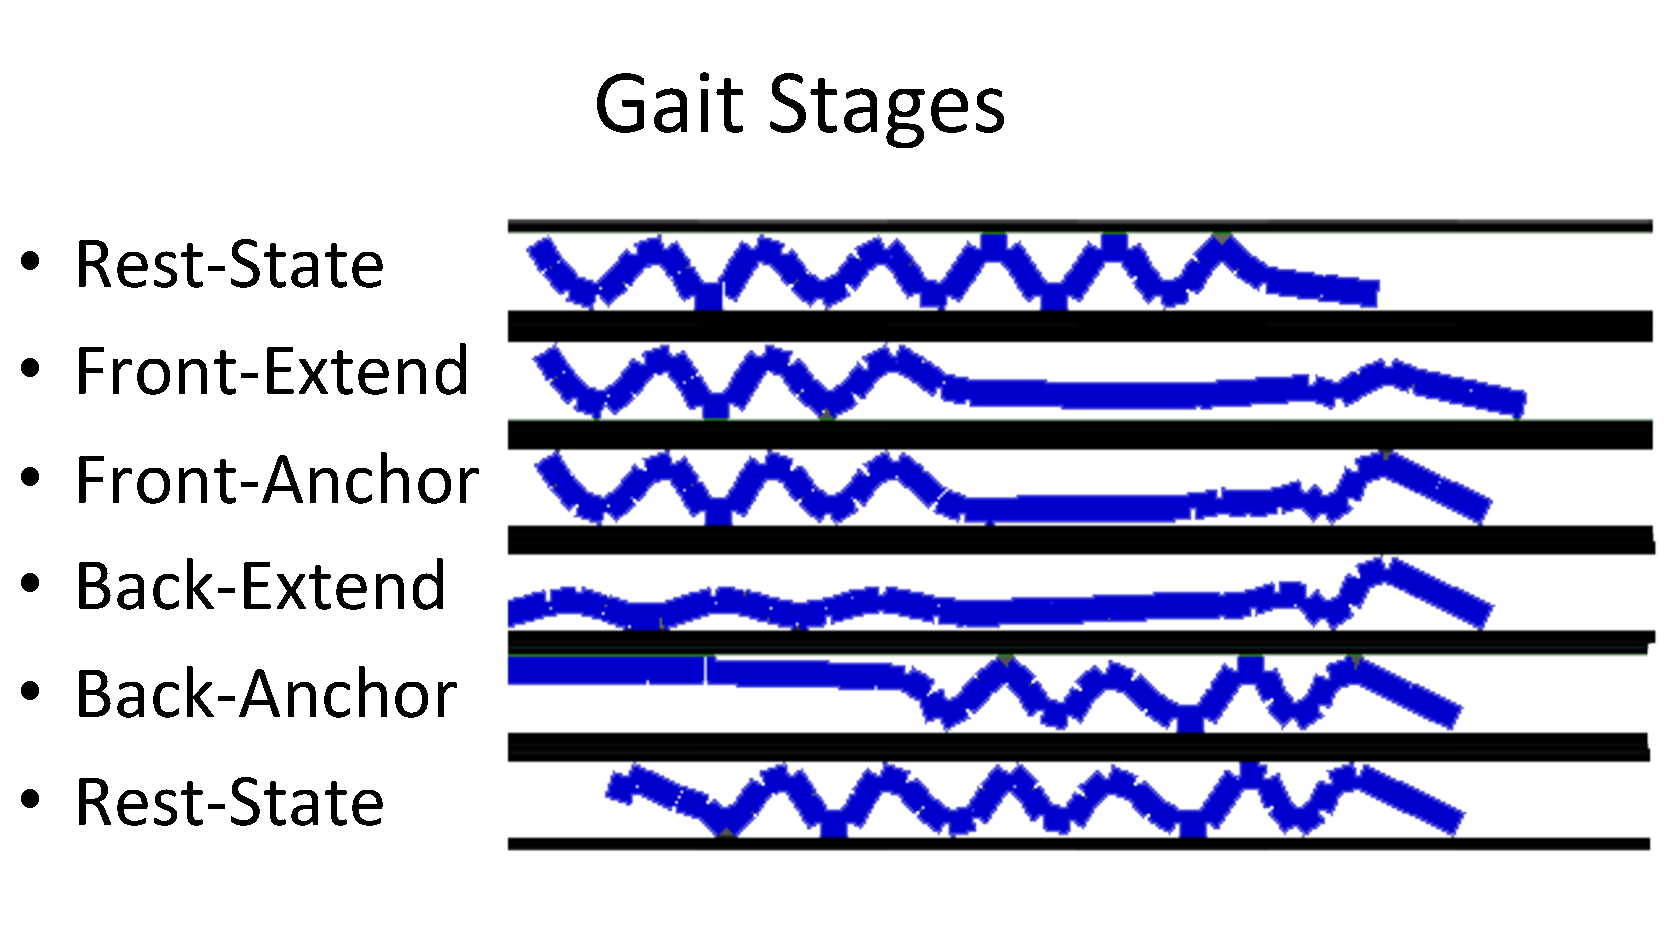
\includegraphics[keepaspectratio,width=\textwidth,height=0.75\textheight]{PastedGraphic5.pdf}
\label{pastedgraphic5.pdf}
\end{figure}



\begin{figure}[htbp]
\centering
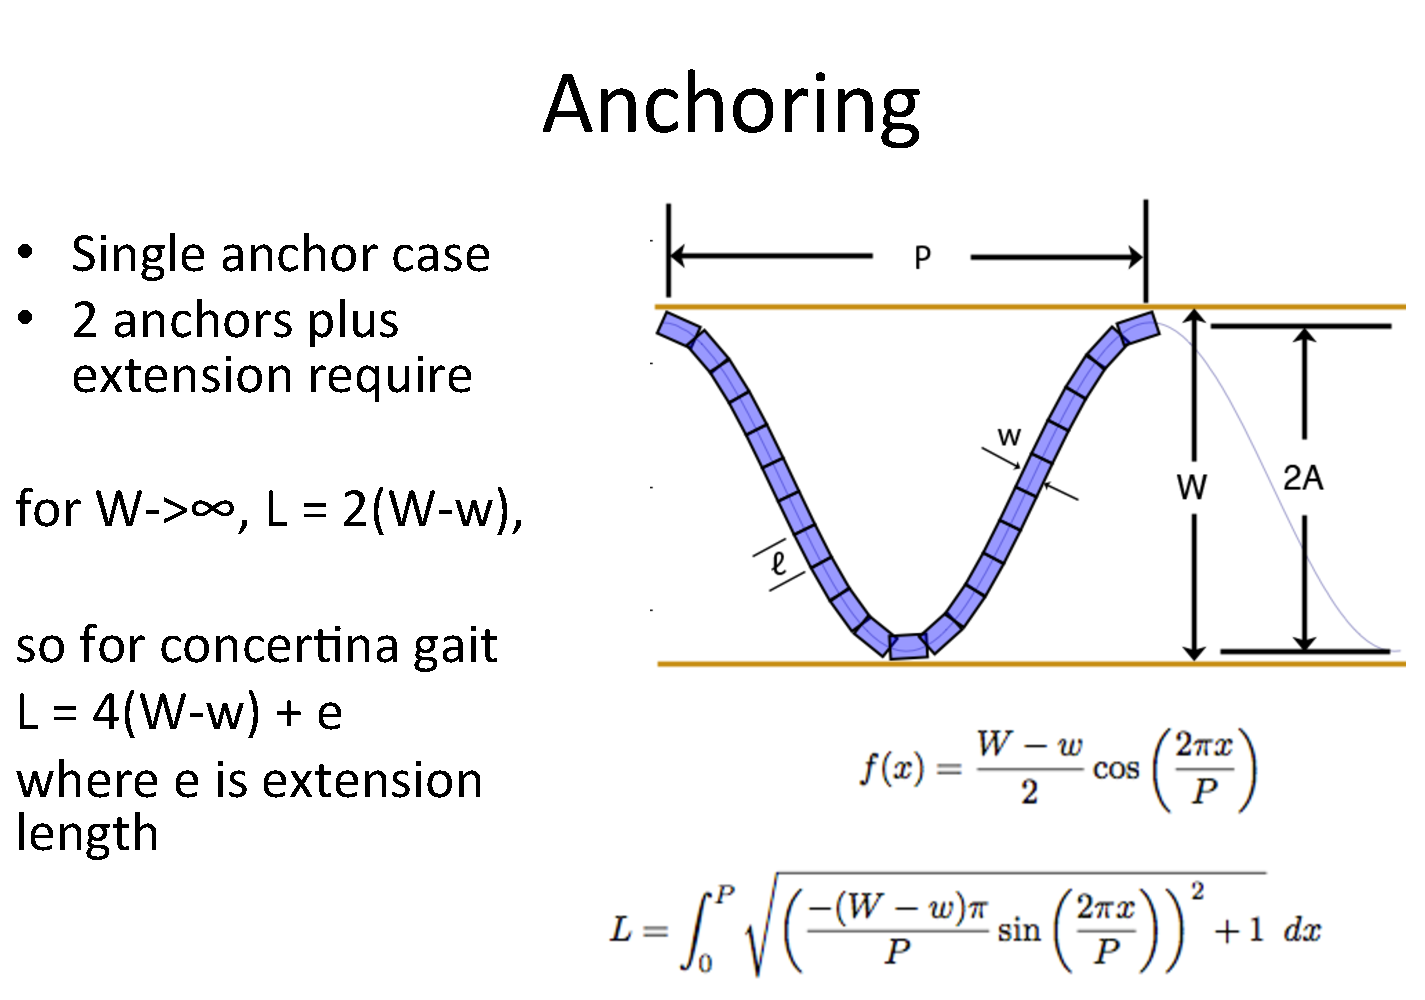
\includegraphics[keepaspectratio,width=\textwidth,height=0.75\textheight]{PastedGraphic6.pdf}
\label{pastedgraphic6.pdf}
\end{figure}




\section{Control Methodology}
\label{controlmethodology}

Backbone curve fitting, IK method, segmented behaviors

\section{Behaviors}
\label{control:behaviors}

Locomotion steps, extensions, path-following, anchoring

\section{Problem}
\label{control:problem}

FIXME: Related work and our contrasted difference. What can we achieve that others cannot. Why is our approach better for this particular case? 

In order to successfully control a snake robot and have it move through the environment, we need a solution for locomotion, motion planning, and handling collisions. Since we have no exteroceptive sensors, this makes the problem challenging. The robot is unable to sense what is right in front of it and must move blindly. The snake could move into open space or collide with obstacles.

Part of the challenge is having no external sensors and the other part is general task-oriented control of a hyper-redundant robot. There are many biologically-inspired locomotion strategies that live snakes in nature use to move throughout the environment. The closest biological gait solution to moving in confined environments is the concertina gait shown in \autoref{bio}.

\begin{figure}[htbp]
\centering
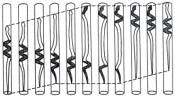
\includegraphics[keepaspectratio,width=400pt,height=0.75\textheight]{concertina_gait_Gans1980.jpg}
\caption{Biological Concertina Gait of a Snake in a Confined Space. Image taken from \textbackslash{}cite\{Gans:1980p775\}}
\label{bio}
\end{figure}



This gait is characterized by a concertina motion of alternating extensions and contractions that result in a forward movement. The snake body pushes against both sides of the walls establishing anchors that allow the snake to alternate between pulling and pushing itself forward. Success of locomotion depends on the snake establishing high friction contacts with the environment with which to push and pull.

However, the differences between a real snake and our robot snake make a true implementation impossible. A real snake has the luxury of vision and olfactory sensors to provide early motion planning and a rich tactile sensing surface skin to provide feedback to its control system. Our robot snake has only the benefit of internal proprioceptive joint sensors. If we knew the exact width of the pipe walls, we could prescribe the perfect concertina motion to move through the environment smoothly.

A simple approach to making the fully anchored concertina posture, we could use the following equation:


\begin{equation}
\label{eq:naiveconc}
\alpha_i = A * \cos \left( \frac{ 2 \pi if}{N} \right)
\end{equation}


where $\alpha_i$ is the commanded joint angle for joint $i$, $f$ is the frequency or the number of sinusoidal cycles per unit segment length, $A$ is the maximum joint command amplitude, and $N$ is the number of segments on the snake. Since there are $N$ segments, there are $N-1$ joints. Therefore, $i \in [0,N-1)$. This equation requires some tuning to give the right results and can result in bad postures such as that shown in \autoref{naiveconc}. In order to effect locomotion, a sliding Gaussian mask should be applied to the joint command output to transition parts of the snake between fully anchored to fully straight to reproduce the biological concertina gait.

\begin{figure}[htbp]
\centering
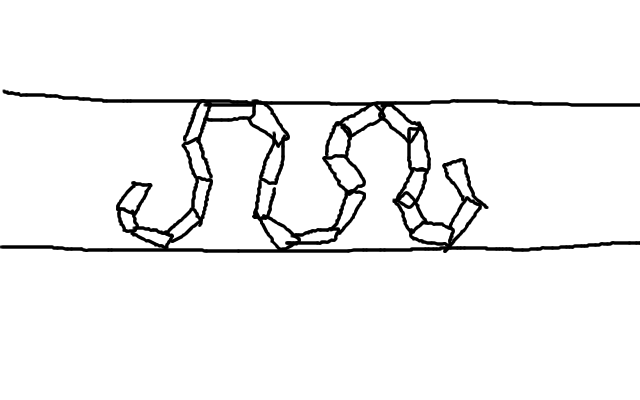
\includegraphics[keepaspectratio,width=400pt,height=0.75\textheight]{2_problem_1.png}
\caption{Improperly tuned concertina posture using equation \autoref{eq:naiveconc}.}
\label{naiveconc}
\end{figure}



The difficulty of this approach is that we need a priori knowledge of the pipe width, the configuration of the snake needs to be tuned by hand for the particular snake morphology, and there is no sensory feedback to this implementation. With no feedback, there is no adaptive behavior possible. We need an approach that will work in environments of unknown and variable pipe width. Our robot needs to be able to adapt its locomotion to the width of the pipe.

Our desire is to be able to prescribe any type of snake posture, for any anchor width and any snake segment length or parameters, and have the snake automatically assume that posture. In order to do this, we need a means of specifying the posture and an inverse kinematics method for achieving that posture.

For both of these requirements, we use the backbone curve-fitting methodology first described by \textbackslash{}cite\{Chirikijan:1995p774\}. This method of control is to produce a parameterized curve that represents the desired posture of the snake over time. Over time the curve changes to reflect desired changes in the snake posture. Snake backbone curve fitting is achieved by finding the joint positions that best fit the snake body onto the curve. This is found either by direct calculation or a search algorithm.

An example of backbone curve fitting can be seen in \autoref{oneperiod}. The parameterized curve is shown in light blue in the background. The blue snake body in the foreground is fitted onto the curve using an iterative search algorithm for each consecutive joint. 

\begin{figure}[htbp]
\centering
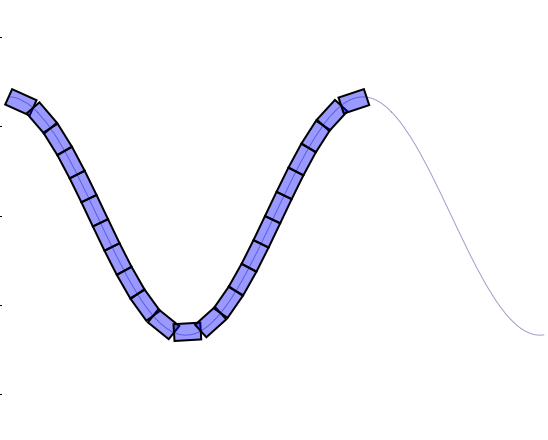
\includegraphics[keepaspectratio,width=400pt,height=0.75\textheight]{OnePeriodCurve.png}
\caption{One period sine curve}
\label{oneperiod}
\end{figure}



A typical application would be to specify the posture of the snake using a sinusoidal curve and then applying an inverse kinematics technique to fit the snake to the curve. The problem can be formulated iteratively as follows: for joints $i \in [0,k]$ and joint pose in space $p_i = \langle x_i,y_i,\theta_i \rangle $ are on the curve $\beta$ with parameter $t_i$, find the joint angle $a_k$ such that $p_{k+1}$ is on the curve $\beta$ and $t_k < t_{k+1}$.

For the equation $\beta$ defined as:


\begin{equation}
\label{eq:curve1}
y = A\sin(2\pi x)
\end{equation}


the equation is monotonic along the $x$ axis, so satisfying the criteria $t_i < t_{i+1}$ is the same as satisfying $x_i < x_{i+1}$. 

If the length a of snake segment is $l$, we specify a circle equation centered at the joint position $(x_i,y_i)$ with the following:


\begin{equation}
\label{eq:IKcircle}
(x-x_i)^2 + (y-y_i)^2 = l
\end{equation}


Finding solutions for the simultaneous equations \autoref{eq:curve1} and \autoref{eq:ikcircle} will give us possible solutions to $x_{i+1}$ and $y_{i+1}$. For these two sets of equations, there are always at least 2 possible solutions. We need only select the solution that satisfies the invariant condition $x_i < x_{i+1}$. There may be more than solution. In which case, we select the $x_{i+1}$ where $(x_{i+1}-x_i)$ is the smallest. This prevents the snake from taking shortcuts across the curve and forces it to fit as closely as feasibly possible to the parameterized curve given the snake robot's dimensions.

The above simultaneous equations do not have closed-form solutions and instead must be solved numerically. This can be computationally expensive using general equation solvers. Instead we propose a more specialized solver for this particular problem.

We choose a series of uniform samples $(q_0 ... q_k ... q_M)$ around a circle of radius $l$ centered at $(x_i,y_i)$ such that all points $q_k$ have $x_k >= x_i$. We are looking for instance of crossover events where the line segment $(q_k,q_{k+1})$ crosses over the curve $\beta$. Given at least one crossover event, we do a finer search between $(q_k, q_{k+1})$ to find the closest point on the circle to the curve $\beta$ and accept that as our candidate position for joint point $p_{k+1}$. As long as we assume that the curve $\beta$ is monotonic along the x-axis and a point of the curve $\beta$ can be computed quickly given an x-value, this is a faster method of computing intersections of the circle with the backbone curve than a general numerical solver.

For instance, in \autoref{plot_3}, we show a curve $\beta$ described by a sine curve and a series of circles intersecting with the curve that indicate candidate locations for placing the subsequent joint on the curve. These are used to determine the appropriate joint angles to fit the snake onto the curve.

Now that we have a means of changing the snake's posture to any desired form given a parameterized, monotonic curve that describes the posture, we now need to form an anchoring approach that will work for arbitrary pipe widths.

\section{Anchoring}
\label{anchoring}

In order to fit the anchor points to a pipe of unknown width, we need some way of sensing the walls. Since we have no exteroceptive sensors, the best way of sensing the width of the walls is by contact. Since we have no direct contact sensor per se, we must detect contact indirectly through the robot's proprioceptive joint sensors.

Using the backbone curve fitting approach, we take one period of a sine curve as the template form we wish the robot to follow. We then modify this sine period's amplitude, at each step refitting the snake robot to the larger amplitude, until the robot make's contact with the walls. This establishes two points of contact with the wall which assist in immobilizing the snake body.

It is clear from \autoref{oneperiod} that as the amplitude of the curve increases, more segments are needed to complete the curve. If the sine curve is rooted at the tip of the snake, this results in the curve translating towards the snake's center of mass. Instead, we root the sine curve on an internal segment, as seen in \autoref{anchor1}, so that the position of the anchor points remain relatively fixed no matter the amplitude and the number of segments required to fit the curve.

\begin{figure}[htbp]
\centering
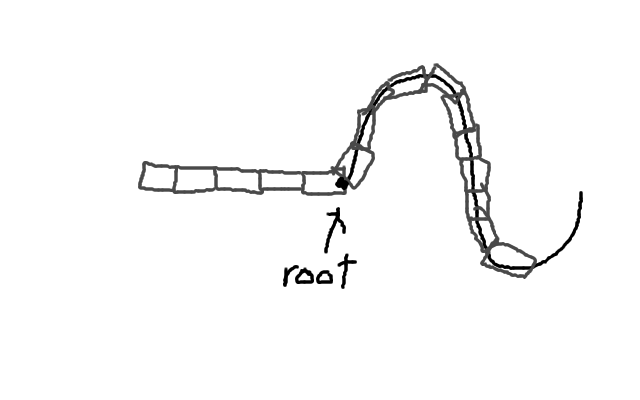
\includegraphics[keepaspectratio,width=400pt,height=0.75\textheight]{2_anchoring_1.png}
\caption{Anchor with not enough segments}
\label{anchor1}
\end{figure}



\begin{figure}[htbp]
\centering
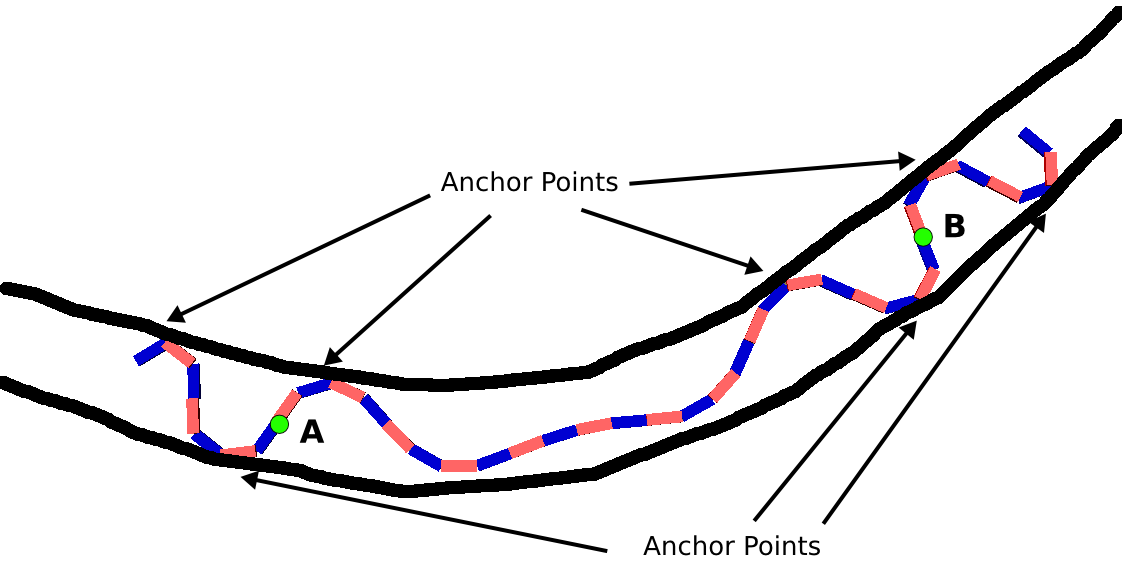
\includegraphics[keepaspectratio,width=400pt,height=0.75\textheight]{ref_points_pose2.png}
\caption{Anchor Points}
\label{fig:anchor_points}
\end{figure}




Two points of contact are not statically stable if we disregard friction. Though friction exists in our simulation and in reality, we do not rely on it to completely immobilize our robot. Our normal forces are often small and the dynamic and transient forces can easily cause a contact slip. Therefore, we need at least 3 contact points to consider an anchor to be statically stable.

One way to achieve this is by adding new sine period sections to create another pair of anchors. The amplitude of the new sine period is separate from the previous anchor's amplitude and is represented by a new curve attached to the previous one. This way the amplitudes remain independent. The equation to describe two sets of sine period curves with independently controlled amplitudes are as follows:


\begin{equation}
y = \mathrm{U}(x)  \mathrm{U}(2\pi-x) A_1 \sin(fx) + \mathrm{U}(x-2\pi) \mathrm{U}(4\pi-x) A_2 \sin(fx)
\end{equation}


where $f$ is the frequency and $\mathrm{U}(x)$ is a unit step function. Or to generalize for $N$ periods and $N$ pairs of anchor points:


\begin{equation}
y = \sum_{i=0}^{N-1} \mathrm{U}(x-i 2\pi) \mathrm{U}((i+1) 2\pi-x) A_i \sin(fx)
\end{equation}


for each anchor curve amplitude $A_i$.

So now that we have the means to control the amplitude of our anchor points, we need some means of detecting that a contact is made and another to make sure the anchor is secure. 

Our approach is to gradually increase the amplitude of an anchor curve until contact with both walls has been made. We will continue to increase the amplitude until we see significant joint error occur when fitting to the curve. If the amplitude because larger than the width of the pipe, the snake will attempt fitting to a curve that is impossible to fit to and will experience a discrepancy in its joint positions compared to where it desires them to be.

The structure of this error will normally take the form of one or two large discrepancies surrounded by numerous small errors. This reflects that usually one or two joints will seriously buckle against the wall, while the rest of the surrounding joints can reach their commanded position without disturbance. An example of an anchor curve with larger amplitude than the width of the pipe is shown in \autoref{anchor2}.

\begin{figure}[htbp]
\centering
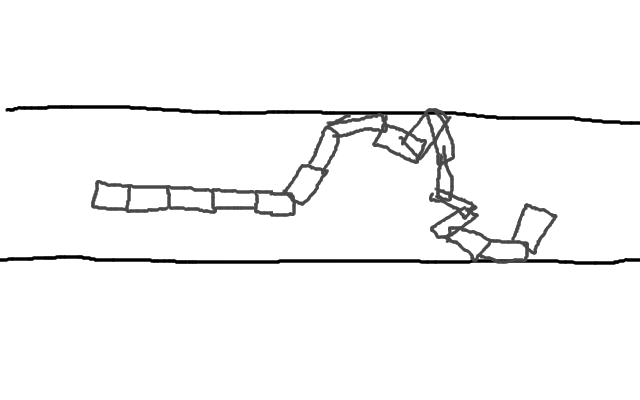
\includegraphics[keepaspectratio,width=400pt,height=0.75\textheight]{2_anchoring_2.png}
\caption{Anchor with amplitude larger than pipe width.}
\label{anchor2}
\end{figure}



The contact is flagged once the maximum error reaches a certain threshold across all the joints of the anchor curve. Of the joints $M$ of the anchor curve and the error $e_j$, if there exists $e_j > 0.3$ radians, than we flag a contact. It isn't so much that we are detecting a contact but a minimum pushing threshold against the wall. The robot is pushing hard enough to cause joint error over an experimentally determined threshold.

If $j_k$ through $j_{k+M}$ are the joints comprising the fitted anchor curve, the error of one joint is defined by $e_k = |\phi_k-\alpha_k|$. The maximum error is defined by $e_{max} = \mathrm{max}(e_k, e_{k+1} \cdots e_{k+M-1}, e_{k+M})$.

The amplitude is initially changed by large increments to quickly find the walls. Once the threshold has been reached, the current and last amplitude are marked as the max and min amplitudes respectively. We then proceed to perform a finer and finer search on the amplitudes between the max and min boundaries until we reach a snug fit that is just over the error threshold. This is a kind of numerical search(?).

The pseudocode for this algorithm is as follows:


\begin{algorithm}
\caption{Anchor Fitting}          % give the algorithm a caption
\label{alg:anchor}
\begin{algorithmic}

\State $\hat{A} \Leftarrow 0$
\State $A_{min} \Leftarrow 0$
\State $A_{max} \Leftarrow \infty$
\State $\delta A \Leftarrow 0.04$

\While{$ (A_{max}-A_{min} >= 0.001) \And (\delta A >= 0.01)  $} 

  \State $\hat{A} \Leftarrow \hat{A} + \delta A$
  \State $e_{flag} \Leftarrow \mathrm{setAnchorAmp}(\hat{A})$
 
  \If { $\neg e_{flag}$ }
    \State $A_{min} \Leftarrow \hat{A}$
  \Else
    \State $A_{max} \Leftarrow \hat{A}$
    \State $\delta A \Leftarrow \delta A / 2$
    \State $\hat{A} \Leftarrow A_{min}$
    \State $\mathrm{setAnchorAmp}(\hat{A})$

  \EndIf

\EndWhile

\end{algorithmic}
\end{algorithm}


The main objective of this code is to reduce the difference between maxAmp and minAmp as much as possible. minAmp and maxAmp are the closest amplitudes under and over the error threshold respectively. The function setAnchorAmp() sets the amplitude, performs the curve fitting, and reports back any error condition as described earlier. Once this algorithm is complete, we have made a successful anchor with two contact points under compression without the fitted anchor curve being distorted by joint buckling.

\section{Curves}
\label{curves}

When we describe curves for use in backbone curve fitting, they must be assigned to a frame of reference and usually have a starting point. Most often, the frame of reference chosen is one of the local segment frames on the snake body. However, sometimes we could choose the global frame if we wanted to navigate or probe something specific in the environment. The local frame curves that we use all start from a specific body segment and sprout from that segment like a plant. We say that this curve is rooted in segment X.

\section{Behavior Architecture}
\label{behaviorarchitecture}

Our method of control is a behavior-based architecture that is charged with reading and tasking the servo-based motor controllers of each joint. Each behavior may be a primitive low-level behavior or a high-level composite behavior composed of multiple sub-behaviors. Furthermore, a behavior may have complete control of every joint on the snake or the joints may be divided between different but mutually supporting behaviors. This architecture allows us to achieve a hierarchy of behavior design as well a separation of responsibilities in task achievement. For instance, the back half of the robot could be responsible for anchoring, while the front half could be responsible for probing the environment as seen in the example architecture in \autoref{behaviors1}.

\begin{figure}[htbp]
\centering
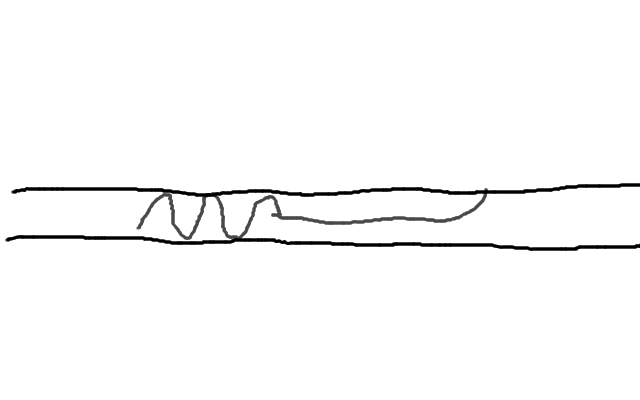
\includegraphics[keepaspectratio,width=400pt,height=0.75\textheight]{2_behaviors_1.png}
\caption{Separation of functionality}
\label{behaviors1}
\end{figure}



Each behavior in the behavior-based architecture is time-driven. It is called periodically by a timer interrupt to compute the next commands for the following time-step. This could be variable time or constant time, but to make our behavior design simple, we use 10ms constant time steps in our simulation.

At each time step, the state of the robot is captured and driven to the behaviors. The data includes a vector of joint angles $\phi_i$, a vector of commanded angles $\alpha_i$, and a vector of maximum torques $m_i$. These values were described in the previous section X. The output of each behavior is a vector of new commanded angles $\hat{\alpha}_i$, a vector of new max torques $\hat{m}_i$, and a vector of control bits $c_i$. The values of $\hat{\alpha}_i$ can be any radian value within the joint range of motion or it can be NULL. Likewise, the new max torque of $\hat{m}_i$ can be any non-negative max torque threshold or NULL. The NULL outputs indicate that this behavior is not changing the value and if it should reach the servo-controller, it should persist with the previous value.

The bits of the control vector, $c_i$ , are either 1, to indicate that the behavior is modifying joint i, or 0, to indicate that it has been untouched by the behavior since its initial position when the behavior was instantiated. This control vector is to signal the activity to parent behavior that this part of the snake is being moved or controlled. The parent behavior does not need to respect these signals, but they are needed for some cases.

Our behavior-based control architecture follows the rules of control subsumption. That is, parent behaviors may override the outputs of child behaviors. Since we can also run multiple behaviors in parallel on different parts of the snake, sometimes these behaviors will try to control the same joints. When this happens, the parent behavior is responsible for either prioritizing the child behaviors or adding their own behavior merging approach.

Asymmetric behaviors that run on only one side of the snake such as the front are reversible by nature. That is, their direction can be reversed and run on the back instead. All behaviors with directional or asymmetric properties have this capability..

Finally, parent behaviors can instantiate and destroy child behaviors at will to fulfill their own control objective. All behaviors are the child of some other behavior except the very top root-level behavior which is the main control program loaded into the robot and responsible for controlling every joint. The root behavior is responsible for instantiating and destroying assemblages of behaviors to achieve tasks as specified in its programming. We will discuss some of these behaviors and child behaviors in the following sections.

\section{Smooth Motion}
\label{sec:smooth}

We desire the motion of our snake robot to be slow and smooth in nature. It does us no benefit for the motion to be sudden and jerky. Moments of high acceleration can have unintended consequences that result in our anchor points slipping. Either collisions with the environment or transient internal dynamics can cause the anchor points to slip.

Our method of ensuring smooth motion is to take the initial and target posture of the joints of the snake, perform linear interpolation between the two poses, and incrementally change the joint angles along this linear path. For instance, if the initial joint angles are ${s_0 ... s_n}$ and the target joint angles are ${t_0 ... t_n}$, the interpolated path for each joint $j$ is found by $g_{jr} = s_j + (t_j – s_j) * (r/100)$ for $r \to {0, 100}$, for 100 interpolated points on the linear path. The resultant motion is a smooth transition from initial to target posture as seen in \autoref{smooth1}.

\begin{figure}[htbp]
\centering
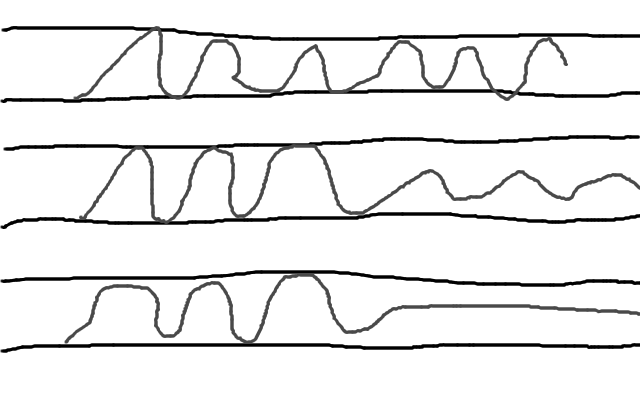
\includegraphics[keepaspectratio,width=400pt,height=0.75\textheight]{2_smooth_1.png}
\caption{Smooth motion from interpolation of posture.}
\label{smooth1}
\end{figure}



This is the definition of the HoldTransition behavior. When it is instantiated, it is given an initial pose vector $S$ and target pose $T$, where some values of $t_i$ in $T$ and $s_i$ in $S$ may have NULL for no command. At each step of the behavior, using the equation $g_{jr} = s_j + (t_j – s_j) * (r/100)$, $r$ is incremented to compute the new joint command. If $t_j$ is NULL, then $g_{jr} = s_j$. Once $r = 100$, it returns True on step() and on all subsequent steps, $g_j = t_j$.

\section{Behavior Merging}
\label{sec:merge}

There are a few methods for merging behaviors that overlap in some way. One way of the previous section is for two behaviors to overlap temporally and using the HoldTransition behavior to handle a smooth transition from one configuration to another.

In the event that two behaviors control adjacent sets of joints or overlap their control in some way, a conflict resolution is method is needed to not only select the proper command for contested joints, but to prevent either behavior from negatively affecting functionality of the other by modifying any positional assumptions or introducing any unintended forces or torques to the other side.

A common occurrence is that two behaviors may try to control the same set of joints at the same time or otherwise. This is a conflict that requires resolution by the parent behavior. In this section we present three different ways to merge the outputs of different behaviors as means of conflict resolution. They are, in the order presented, the precedence merge, the splice merge, the convergence merge, and the compliance merge respectively.

Given that all child behaviors have an ordering, the default resolution method is to take the first behavior's control output over all others. This is called precedence merging. An ordering is always specified by the parent at the time it instantiates the child behaviors. If the first behavior's output is NULL, then it goes to the next behavior and so on until a non-NULL value is found or the last behavior returns a NULL, in which case the parent also returns a NULL unless the parent otherwise specifies.

Precedence merging can be crude when trying to maintain a stable and immobilized position in the environment. Sudden changes at the behavior-boundary can cause jarring discontinuities on the snake's posture and result in loss of anchoring as seen in \autoref{merging1}. A more finessed approach would disallow these discontinuities and provide a non-disruptive merging. The first approach that does this is the splice merge.

\begin{figure}[htbp]
\centering
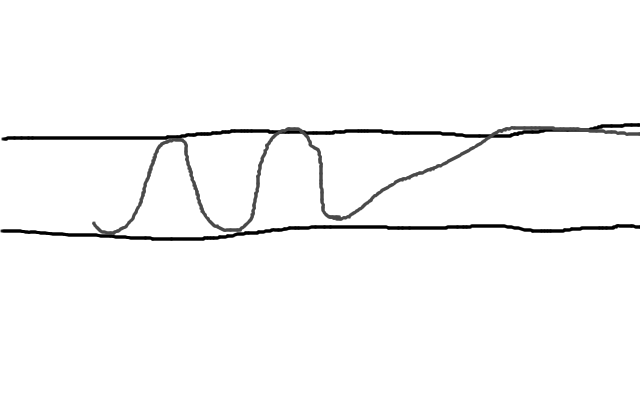
\includegraphics[keepaspectratio,width=400pt,height=0.75\textheight]{2_merging_1.png}
\caption{Discontinuity in behaviors results in clash of functionality.}
\label{merging1}
\end{figure}



In the event that two behaviors overlap, we have the option of having a hard boundary between the behaviors centered on a single joint. Except in the rare case that both behaviors want to command the splice joint to the same angle, it is highly likely that the merge will be discontinuous. In order to ensure that positional assumption is maintained for both behaviors, the behaviors must be spliced so that neither behavior disrupts the other.

If the splice joint is $j_s$, behavior A controls joints $j_0$ through $j_s$, behavior B controls joints $j_s$ through $j_{N-1}$, $S_{s-1}$ is the body segment connected to $j_s$ in behavior A, and $S_s$ is the body segment connected to $j_s$ in behavior B, we have the situation shown in \autoref{merging2}a. If behavior A commands $j_s$ to $\alpha_a$ to put segment $S_s$ in the position shown in \autoref{merging2}b and conversely, if behavior B commands $j_s$ to $\alpha_b$ to put segment $S_{s-1}$ in the position shown in \autoref{merging2}c, the two behaviors can be spliced discontinuously with no disruption to either behavior by setting $j_s$ to $\alpha_s = \alpha_a + \alpha_b$. The result is shown in \autoref{merging2}d.

\begin{figure}[htbp]
\centering
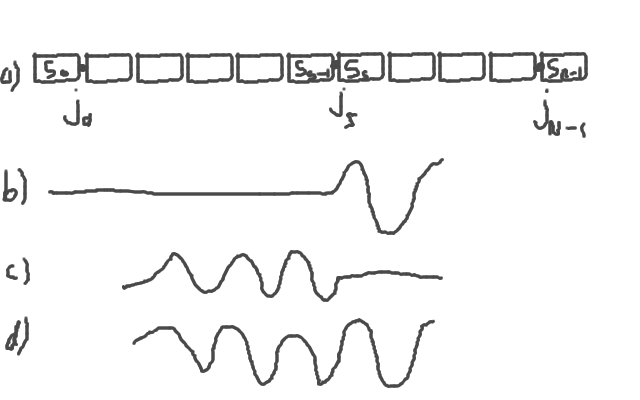
\includegraphics[keepaspectratio,width=400pt,height=0.75\textheight]{2_behaviors_2.png}
\caption{Splice joint and connecting segments.}
\label{merging2}
\end{figure}



This is the behavior splicing approach because it stitches the behaviors together in a clinical way to ensure proper functionality of both. Its primary role is to connect behaviors with discontinuous conflicts on the behavior boundary and whose positions must be maintained for functional purposes. For more fuzzy continuous boundaries, we use the convergence merging approach.

For the two behaviors shown in \autoref{merging3}a and \autoref{merging3}b, the resultant convergence merge is shown in \autoref{merging3}c. For this approach, there is no discrete boundary but one behavior converging to another over several joints. For a given joint $j_i$ somewhere in this convergence zone, and the commanded values for behaviors A and B being $\alpha_a$ and $\alpha_b$, the converged command value for $j_i$ is computed by:


\begin{equation}
\label{equ:slide}
\alpha_i = \alpha_a + (\alpha_b – \alpha_a) / ( 1 + \exp(i-c))
\end{equation}


where $c$ is a calibration parameter that controls the magnitude and location of the convergence along the snake. As $c \to +\infty$, $\alpha_i \to \alpha_b$. As $c \to -\infty$, $\alpha_i \to \alpha_a$. In practice, $|c| < 20$ is more than sufficient for complete convergence to one behavior or the other. The $i$ parameter in the exponent ensures that the convergence value is different for each of the neighboring joints. This produces the effect shown in \autoref{merging3}c.

\begin{figure}[htbp]
\centering
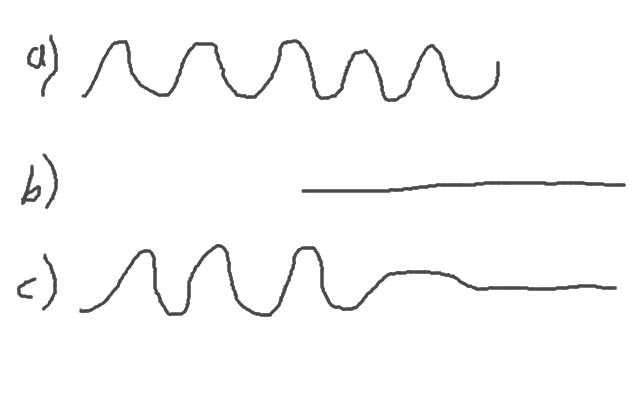
\includegraphics[keepaspectratio,width=400pt,height=0.75\textheight]{2_behaviors_3.png}
\caption{Convergence merge.}
\label{merging3}
\end{figure}



If we modify $c$, this gives us a control knob on the merge and can be moved up and down. If we move $c \to +\infty$, behavior B takes complete control of the snake. If we move $c \to -\infty$, behavior A takes control of the snake. $c$ can be changed over time to create a sliding transition effect with a convergence boundary. In fact, this is the basis for a behavior called HoldSlideTransition.

A fourth and final way for two behaviors to be merged is the compliance merge. This is the case where two behaviors are not adjacent but are far away from each other, but still interfere with each other somehow by inflicting unwanted forces and torques between the behaviors.

A compliance merge resolves this by selecting a group of joints between the two behavior's joint sets to be compliant or non-actuated. This has the result of absorbing any forces or torques transmitted by either behaviors and mechanically isolating one side of the snake from the other. An example is shown in \autoref{merging4}.

\begin{figure}[htbp]
\centering
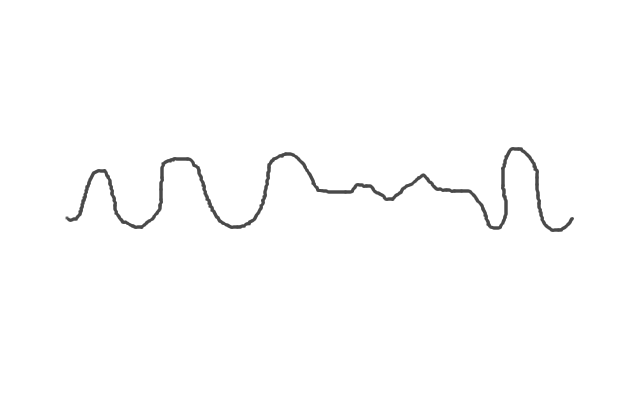
\includegraphics[keepaspectratio,width=400pt,height=0.75\textheight]{2_behaviors_4.png}
\caption{Compliance merge.}
\label{merging4}
\end{figure}



\section{Compliant Motion}
\label{compliantmotion}

In the previous section, we mentioned compliance but not our implementation. Compliant motion is a much used technique in robotics and has been discussed widely (cite). The two approaches are either passive or active compliance. Our approach is to use passive compliance since we have no means to detect contact or sense obstacles.

Passive compliance is achieved by changing the settings on the max torque parameter of each joint's servo controller. We use a high setting for active motion, a low setting for compliant motion, and zero for keeping the joint unactuated.

Besides using a compliance merge to mechanically isolate two behaviors, we also use compliance as an exploration strategy. Since we have no exteroception, the only way to discover walls and obstacles is to collide with them. Compliant impacts with obstacles have a couple benefits. It prevents the force of the impact from transmitting to the body of the snake and possibly causing anchor slip. It also allows the joints of the snake to give out and take the shape of the environment around it. 

This latter benefit is one of our primary means of sensing and exploring the environment. By passively letting the snake robot assume the shape of the environment, it guides our mapping and our locomotion. Until we have mapped out open space and boundaries, we have no way of directing our robot towards them beyond colliding with the unknown.

\section{Stability Assurance}
\label{sec:stability}

In a previous section on smooth motion, we discussed an interpolation technique to smoothly transition from one posture to another. The primary motive of this was to keep the parts of the snake body that are immobilized from being destabilized by transient forces and causing anchor slip. Static forces from prolonged pushing against an obstacle or wall are a separate matter.

For a pose transition that has a sufficiently large number of interpolation steps of sufficiently large duration, we can reasonably be assured that no transient forces from dynamics or collision will cause anchor slip because we are moving very very slowly. However, sufficiently long transition times for reliability may be impractical for applications, since times for a simple transition can be upwards of 1--2 minutes using a conservative approach. For a robot that performs hundreds of moves that require transitions, this is an unacceptable approach.

If we focus on being able to detect transient forces on the snake body instead, we can use this to control the speed of our movements instead of a one-size-fits-all approach of long transition times for all motion. We have developed a heuristic technique to do just this.

Our approach is to use our only source of information, joint angle sensors, as make-shift stability monitors of the entire snake. That is, if all the joints stop changing within a degree of variance, we can call the whole snake stable. Once we have established that the snake is stable, we can perform another step of motion. 

For each, we compute a sliding window that computes the mean and variance of the set of values contained in. If at every constant time step, we sample the value of some joint $i$ to be $\phi_{it}$, then we compute:


\begin{equation}
\mu = \sum_{t = j-K}^{j} \frac{\phi_{it}}{K}
\end{equation}
\begin{equation}
\sigma^2 = \sum_{t=j-K}^{j} \frac{(\phi_{it} – \mu)^2}{K}
\end{equation}


$K$ is the width of the sliding window or the sample size used for computing the variance. This and the time step size $\delta t$, are used to determine the resolution and length of variance computation. In our implementation, with some exceptions, we use $\delta t = 1\mathrm{ms}$ and $K = 20$. That is, for $N$ joints, we compute the variance of each joint's angle for the last 20 readings once every 1ms. This may be changed and retuned depending on the available computing resources, the resolution of the sensors, and the sensor's sample rate.

Finally, we can determine if the snake is stable if all of the joint variances fall below a threshold $S_v$ and stay that way for over time $S_t$. In our case, we set $S_v = 0.001$ and $S_t = 50\mathrm{ms}$.

We are primarily interested in preventing anchor slip. Most often, it is not necessary to wait for the entire snake to hold still before moving. Instead, we can focus just on the joints in the neighborhood of the anchor points. By computing just the variances of the joints in the local neighborhood of the anchor points, we can determine local stability. Using local stability, we gain some confidence that our anchor points do not slip between motion steps.

In order to use this concept of local stability, we need to have some indication of which joints to monitor and which to ignore. Fortunately, the control vector c, output of the behaviors mentioned in a previous section, is just the kind of information we need to know where to direct our local stability attention. If the values of a control vector indicate `0', this means that these joints are not modified by the behavior and should remain stable before performing another move step. If the values are `1', these joints are actively modified by the behavior and we should not expect these joints to remain stable between move steps. The behavior prescriptively tells us how it should behave and the stability system processes it to accommodate.

\section{Adaptive Step}
\label{adaptivestep}


%Show the behavior sequence in high-level terms.  Show graphics.

%Explain each behavior step in terms of the concepts we already learned.


Using these tools at our disposable, we can now build a suitable locomotion behavior for an unknown pipe with no exteroception. The entirety of our designed behavior is shown in \autoref{adaptive_step} and is called the adaptive concertina gait, a biologically-inspired gait based on the concertina gait but modified for the change in sensors. The behavior is divided into 6 states, and each level of \autoref{adaptive_step} shows one of those states. We describe the states as follows:

\begin{figure}[htbp]
\centering
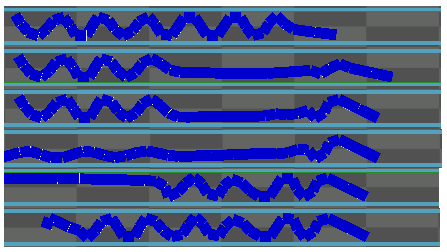
\includegraphics[keepaspectratio,width=400pt,height=0.75\textheight]{AdaptiveStep.png}
\caption{Adaptive Step Concertina Gait}
\label{adaptive_step}
\end{figure}



1) Rest-State (Initial): Rest-State is the initial fully anchored posture of the snake robot. This is our initial pose and it acts as a stable platform from which exploratory or probing behaviors can be executed to sense the environment with little chance of slips or vibration due to the multiple anchor contact points. There is no other action here than to hold the posture that it was already in. The Rest-State is the initial state and the final state of the concertina gait.

2) Front-Extend: In the Front-Extend state, the forward segments are gradually transitioned from their initial position to a straight-forward position. The joints are compliant to the boundaries of the environment to accommodate turns in the pipe.

3) Front-Anchor: The Front-Anchor state takes the extended portion of the snake and attempts to establish an anchor to the pipe as far forward as possible. The locomotion distance is maximized the further forward the front anchor is.

4) Back-Extend: The Back-Extend state follows a successful Front-Anchor event. All anchors established in the back segments are gradually extended until they are straight. Again, the joints are compliant so that they can conform to the walls of the environment.

5) Back-Anchor: The Back-Anchor state involves establishing multiple anchors with the remainder of the body segments.

6) Rest-State (Final): Upon conclusion of the Back-Anchor state, a single step of the adaptive concertina gait is complete and the snake is now in the Rest-State. From here we can do probing of the environment or perform another step forward.

A successful transition through all the states results in a single step. Multiple steps are used to travel through the environment. We describe no steering mechanism for this locomotion gait because the robot has no means to sense the environment in front of it. However, the robot's compliant posture will adapt to any junctions or pipe curvature and follow it.

We now describe the implementation of each of these states and their composition of behaviors.

\subsection{Front-Extend}
\label{front-extend}


%GRAPHIC
%Merge(
%FrontExtend ← HoldSlideTransition ← Transition,
%HoldPosition
%)


\begin{figure}[htbp]
\centering
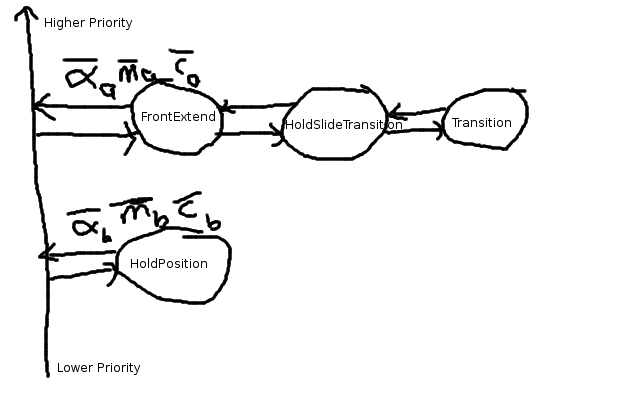
\includegraphics[keepaspectratio,width=400pt,height=0.75\textheight]{2_adaptive_1.png}
\caption{Front-Extend behavior assembly}
\label{adaptive1}
\end{figure}




%Convergence merge of 0.0 extension and anchored state.  Precedence merge of FrontExtend and HoldPosition.  HoldPosition holds back half while FrontExtend controls front.  Passes extended state to HoldSlideTransition.  This manages convergence merge and slide with a Transition behavior to handle each step. 


From the fully anchored Rest-State stage, the goal of the Front-Extend stage is to release the front anchors and stretch the front half of the snake as far forward as possible without compromising the rear anchors. The further forward we can extend, the further the snake can travel in a single step.

If the extended snake arm makes a lateral impact, the walls will guide the movement of the snake but not otherwise hinder the behavior. In the event of an actual obstruction, the tip's movement will stop. We are able to track whether the position of the tip hasn't moved overtime and are able to set a flag to abort the behavior at the current posture.

Its implementation consists of 4 behaviors arranged as shown in \autoref{adaptive1}. We explain each behavior's functionality.

\textbf{HoldPosition:} The purpose of this behavior is to output the same joint commands indefinitely. It is instantiated with a vector of joint commands, and it continues to output these joint commands until termination. In this case, it is instantiated with the entire initial anchored posture of the snake from Rest-State and continues to output this posture. The behavior's output is gradually subsumed by the growth of the FrontExtend behavior in a precedence merge. HoldPosition is placed 2nd in the behavior ordering at the root level for this reason.

\textbf{Transition:} This behavior's purpose is to take an initial and final pose and interpolate a transition between the two, outputting the intermediate postures incrementally. The number of interpolated steps used to transition between the poses is set by the parent behavior. It is often a function of how much difference there is in the initial and final poses. The clock-rate is dependent on the parent behaviors. Once it reaches the final pose, it returns a flag and continues to output the goal pose indefinitely until reset or deleted. Here it is instantiated by the HoldSlideTransition behavior and reset each time it needs to make a new move command.

\textbf{HoldSlideTransition:} This behavior was first mentioned in section \autoref{sec:merge} and implements the equation \autoref{equ:slide}. Its role is to use a convergence merge to transition from one posture to another. The convergence parameter $c$ is incremented over time to slide the convergence from the front to the back of the snake, to smoothly transition from the fully-anchored posture to the back-anchored and front-extended posture.

For each change in $c$, the Transition behavior is set up to interpolate smooth motion between the two postures. Once the Transition behavior completes, $c$ is incremented and Transition is reset to the new initial and final postures. $c$ is changed from 8 to 20 while using the joint numbers as the indices in the convergence merge equation shown in X, assuming that the joint numbering starts at 0 at the front tip. An example of the HoldSlideTransition behavior in action is shown in \autoref{merging3}.

\textbf{FrontExtend:} Finally, the FrontExtend behavior creates HoldSlideTransition as a child behavior and gives it its initial and final posture. It passes through the output of HoldSlideTransition. It also monitors the pose of the snake tip to see if any obstructions are encountered. If the pose remains stationary for a period of time, an obstruction is declared and the behavior is halted. The behavior returns a collision flag.

\subsection{Front-Anchor}
\label{front-anchor}

\begin{figure}[htbp]
\centering
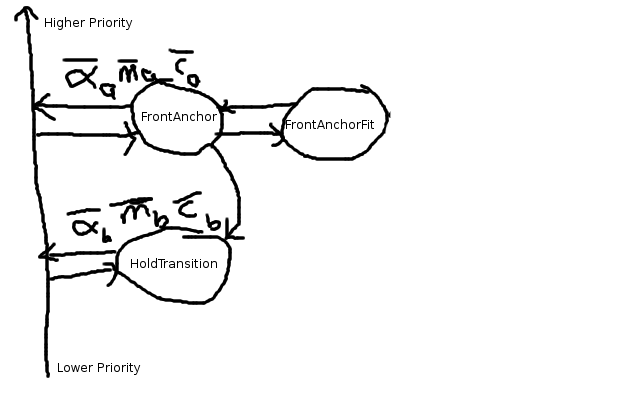
\includegraphics[keepaspectratio,width=400pt,height=0.75\textheight]{2_adaptive_2.png}
\caption{Front-Anchor behavior assembly}
\label{adaptive2}
\end{figure}



%GRAPHIC
%Merge(
%FrontAnchor -> FrontAnchorFit, 
%    |
%   V
%HoldTransition
%)


Once the front-half of the snake has been extended by the Front-Extend stage, the next step is to place the first anchor using the already extended segments. The complete posture of the snake is submitted to a HoldTransition behavior while the front half of the posture is modified by the FrontAnchorFit behavior.

This stage attempts to create a 3-point anchor that is created with the previously extended segments. The anchor is rooted at an internal joint starting from the merge joint 7 giving 8 segments with which to create the anchor. In the event that not enough segments are available to create the full anchor, the anchoring process is restarted with +2 more segments by moving the root inward by 2 joints. 

On successful completion of the 3-point anchor with the available segments, a test is performed to see if the anchor is secure, called a jerk-test. This is accomplished by a sudden rotation of four joints adjacent to the merge joint not on the side of the front anchor. While tracking the position of the anchor segments, if the anchored portion of the snake moves appreciably from the jerk-test, the anchor is deemed insecure, and the anchoring process is restarted with 2 more segments.

Whenever the merge joint is moved inwards, this also results in the contact positions of the anchor points moving inward as well. This can be useful for changing the anchor locations if no stable purchase is found, but also reduces the step distance of the gait by reducing the extension length.

The composition of the behaviors is shown in \autoref{adaptive2} and described as follows:

\textbf{HoldTransition:}
This behavior is originally initialized with the complete posture of the snake at the outcome of the Front-Extend stage. The front portion is laterally modified by the FrontAnchor behavior whenever new changes are required to the front anchor shape. The behavior is stepped and drives the robot joints for smooth transitions.

Though the FrontAnchor behavior has priority over the HoldTransition behavior, FrontAnchor almost never drives an output but instead laterally modifies the HoldTransition behavior. Therefore, the HoldTransition behavior is the primary driver of the snake robot.

\textbf{FrontAnchor:}
This behavior has complete responsibility for the entire anchoring and testing process. It creates a 3-point anchor for static stability instead of the 2-point anchors previously described in section 2.1. This is because this will be the only anchor to the environment in the next stage. Complete secureness is required to avoid any slip conditions.

A 3-point anchor is created with a cosine curve of period 2.5pi shown in \autoref{frontanchor1}. The FrontAnchor behavior gradually increases the amplitude of this curve. As the amplitude increases, more and more segments are required to complete the fit. Should the curve be longer than the available number of segments, the anchoring process is restarted with the merge joint moved back 2 joints.

The anchoring process is halted after search algorithm 2 completes. The behavior then performs a jerk-test to determine if the anchor points are secure. If k'th joint is the merge joint, then the joints [k+1,k+4] are rapidly changed in the following sequence: [(0,0,0,0), (--60,--60,--60,--60), (0,0,0,0), (60,60,60,60)]. These joints are directly controlled by the FrontAnchor behavior to create sudden motion and override the parallel HoldTransition behavior that normally performs smooth motion.

A secure anchor will register little movement in the anchor segments while an insecure anchor will move a great deal. This movement is tracked through kinematics and assumes that the back anchors are secure and stable. Once the deviation in position of the anchor segments is below a certain threshold, than we determine that this is a secure anchor and return success.

\textbf{FrontAnchorFit:}
This behavior is responsible for computing the curve-fitting process described at the beginning of section 2. It determines the correct joint orientations for a given curve. The curve is input by the FrontAnchor behavior and modified accordingly. The FrontAnchorFit behavior performs an efficient curve-fitting process assuming the curve starts rooted at the merge joint on the behavior boundary shown in \autoref{frontanchor1}.

\begin{figure}[htbp]
\centering
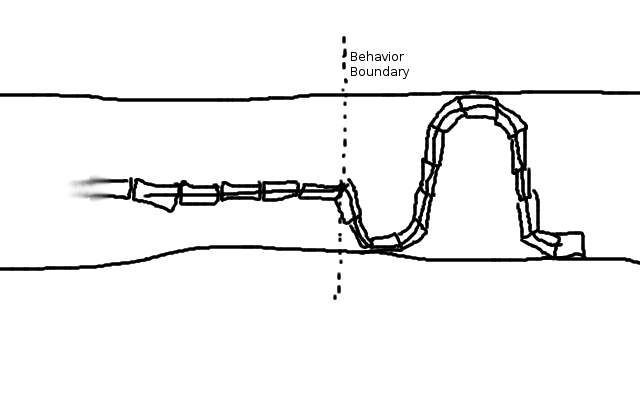
\includegraphics[keepaspectratio,width=400pt,height=0.75\textheight]{2_frontanchor_1.png}
\caption{Posture that creates a 3-point anchor.}
\label{frontanchor1}
\end{figure}



\subsection{Back-Extend}
\label{back-extend}

\begin{figure}[htbp]
\centering
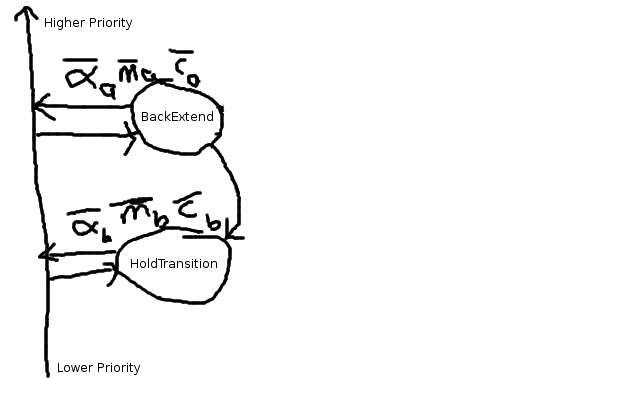
\includegraphics[keepaspectratio,width=400pt,height=0.75\textheight]{2_adaptive_3.png}
\caption{Back-Extend behavior assembly.}
\label{adaptive3}
\end{figure}



%GRAPHIC
%Merge(
%BackExtend
%    |
%    V
%HoldTransition
%)


After the front anchor has been securely established, the next stage's role is to remove the back anchors and extend the back half of the body straight. If the environment prevents the back half from being straight, the joints are compliant to the environment and will extend as far as they are allowed.

The behaviors are shown in \autoref{adaptive3} and described as follows:

\textbf{BackExtend:}
This behavior simply takes all the joints on one side of the merge joint behavior boundary and commands their values to be 0.0. It also sets all of these joints to have low torque to ensure compliant motion. These values are sent laterally to the HoldTransition behavior.

\textbf{HoldTransition:}
This behavior is initialized to the posture from the outcome of the Front-Anchor stage. It receives as input from the FrontExtend behavior, the new straight 0.0 joint positions. It manages the smooth motion from the back anchored position to the back extended position.

\subsection{Back-Anchor}
\label{back-anchor}

\begin{figure}[htbp]
\centering
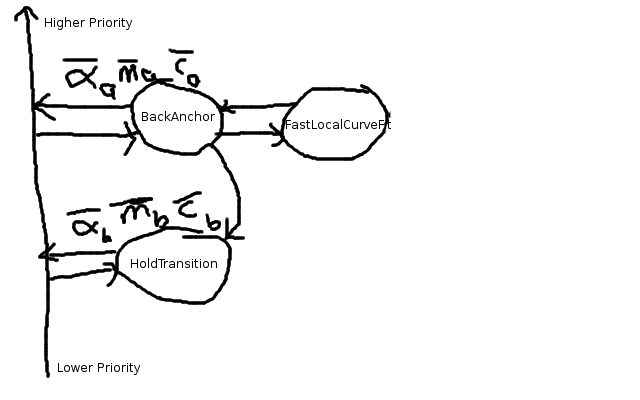
\includegraphics[keepaspectratio,width=400pt,height=0.75\textheight]{2_adaptive_4.png}
\caption{Back-Anchor behavior assembly}
\label{adaptive4}
\end{figure}



%GRAPHIC
%Merge(
%BackAnchor -> FastLocalCurveFit, 
%    |
%    V
%HoldTransition
%)


The purpose of this stage is form the 2-point anchors described in section 2.1 with the remaining extended segments of the back half of the snake. The sine curves are joined together with the front anchor cosine curve to make a continuous splice merge and produce a complete anchored posture of the whole snake.

New pairs of anchor points are created, using one period of a sine curve each, until all of the remaining back segments are used up. At each anchor pair, we use the adaptive anchoring algorithm 2 to detect contacts. However, we do not perform a jerk-test like in the Front-Anchor stage because we only have the front anchor as our reference point and no extra joints to perform the jerking motion. Furthermore, it is not as critical to determine if the back anchors are secure since there are more of them, and we have confidence in the security of our front anchor.

The behaviors are shown in \autoref{adaptive4} and described as follows:

\textbf{HoldTransition:}
This behavior fulfills the same role as all of the other instances. It takes the initial posture at the outcome of the previous stage and maintains that posture until modified by the primary behavior, BackAnchor. It manages the smooth transition between postures.

\textbf{BackAnchor:}
This behavior performs the anchor contact algorithm 2, modifies the curve parameters, and continues to add anchor pairs until it runs out of segments. It creates the FastLocalCurveFit behavior as a child behavior.

\textbf{FastLocalCurveFit:}
This behavior parameterizes the curves representing the series of back anchor curves of varying amplitudes. It is also responsible for efficiently computing the joint positions to fit the snake to the curves. Furthermore, it accepts compliance in the curve-fitting process between each anchor pair. That is, at each merge joint between two anchor pairs, compliance is to find the best anchor posture and the posture is saved for the remainder of the stage.

\section{Analysis}
\label{analysis}

Our theoretical contribution is a quantitative analysis of the trade-space between environmental characteristics, snake robot morphology, and locomotion control parameters. That is, given a snake robot morphology and control parameters, what types of environments can we successfully explore. Conversely, given a specific environment, what robot morphology and control parameters are required to successfully explore it.

First we will perform an analysis of the trade-space for forming a 3-point stable anchor in a smooth pipe. A 3-point anchor is shown in \autoref{param_1} and is the minimum number of contact points required to form a stable anchor. This posture will hold the body of the snake rigid and prevent it from translating or rotating within a threshold of external force and torque.

We will define and quantify the parameters that describe this system: the environment, the robot, and the control.

Our particular environment of a smooth pipe can easily be described with one parameter, the pipe width $W$.

The complete snake robot morphology can be described by 3 parameters: segment width $w$, segment length $l$, and number of segments $n$.

Finally, control of the robot is achieved by fitting the body of the snake onto a curve described by a sinusoid. The parameters for control are the values of amplitude $A$ and period $P$, where $y = A \cos(\frac{2 \pi x}{P})$. 

\begin{figure}[htbp]
\centering
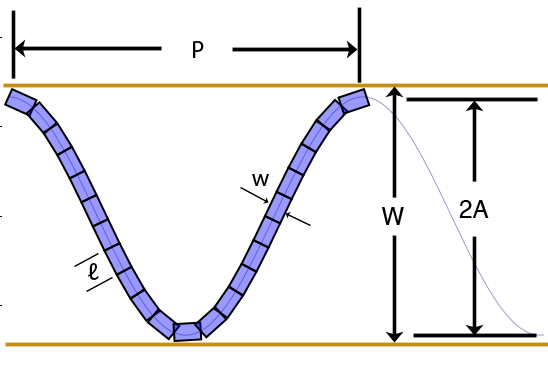
\includegraphics[keepaspectratio,width=400pt,height=0.75\textheight]{CurveDiagram.png}
\caption{Parameterization of 3-point stable anchor in a smooth pipe.}
\label{param_1}
\end{figure}




%\begin{figure}[htb]
%\begin{center}
%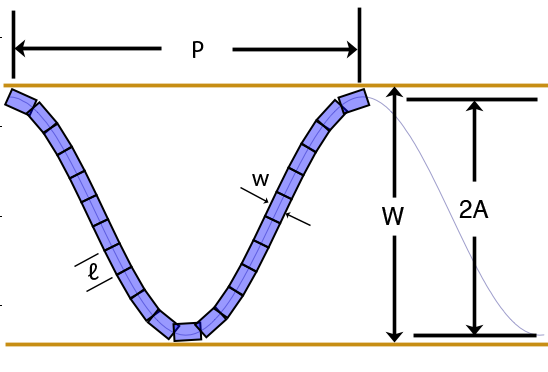
\includegraphics[scale=0.5]{CurveDiagram}
%\end{center}
%\caption{Parameterization of 3-point stable anchor in a smooth pipe.}
%\label{param_1}
%\end{figure}


\subsection{Case: Snake as a Curve}
\label{case:snakeasacurve}

We first consider the degenerate case where $l = 0$, $w = 0$, and $n = \infty $. This results in a snake that has no width and an infinite number of joints. Essentially, the snake body equals the curve equation. Since $w = 0$, this results in $ 2A = W $. This is shown \autoref{deg_1}.

\begin{figure}[htbp]
\centering
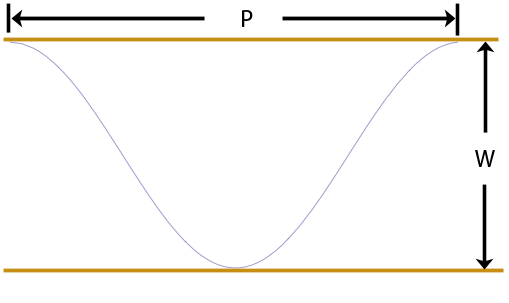
\includegraphics[keepaspectratio,width=400pt,height=0.75\textheight]{DegenerateCurve.png}
\caption{3-point stable anchor with $w = 0$, $l = 0$, and $n = \infty.$.}
\label{deg_1}
\end{figure}



We define $L$ to be the total length of the snake which can be computed from the equation of the curve.


\begin{equation}
f(x) =  \frac{W}{2} \cos \left( \frac{2 \pi x}{P} \right) 
\end{equation}


Equation 1 is the equation of the curve with $P$ the period, $W$ the width of the pipe. We can plug $f(x)$ into the equation for computing arc length shown in Equation 2 and 3:


\begin{equation}
L = \int_{0}^{P} \sqrt{f'(x)^2 + 1} \,\,\, dx
\end{equation}



\begin{equation}
L = \int_{0}^{P} \sqrt{\left( \frac{-W \pi}{P} \sin \left( \frac{2 \pi x}{P} \right)  \right)^2 + 1} \,\,\, dx
\end{equation}


This integration can not be solved analytical and must be solved by plugging in values for $P$ and $W$ and computing $L$ numerically. In our control methodolgy, $P$ is usually held fixed and the width of the environment is always changing, so $W$ is always varying. Here we show a plot holding $P$ fixed for various values while changing the value of $W$ in \autoref{plot_1}.

\begin{figure}[htbp]
\centering
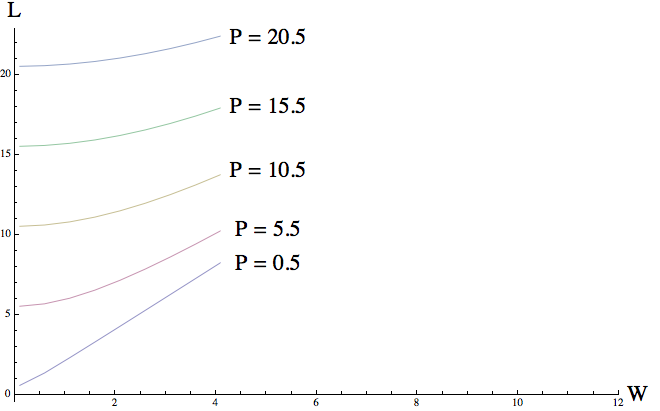
\includegraphics[keepaspectratio,width=400pt,height=0.75\textheight]{2011_01_23_Plot_DegenerateAnchor.png}
\caption{Plot of snake arc length $L$ for various values of $W$ and $P$.}
\label{plot_1}
\end{figure}



This plot shows that when pipe width $W \to \infty$, the length $L$ converges to a constant slope of $\frac{dL}{dW} = 2$ and $L = 2W \,, \forall P$ as $W \to \infty$. This can be seen by approximating the 3-point anchor and cosine curve as a triangle with a base of $P$ and a height of $W$, and the vertices on the anchor points. Increasing $W$ will achieve the above results.

The difference in $L$ becomes large for different values of $P$ when $W$ is small. Once $W$ becomes sufficiently large, $W$ dominates and the period becomes less of a factor. Given that our application involves tight quarters, we are likely to find typical values of $W$ to be small and $P$ will vary depending on the context.

\subsection{Case: Snake with Width}
\label{case:snakewithwidth}

We now consider the case where $l = 0$, $n = \infty$, but $w > 0$. This in effect creates a continuous snake robot with infinite joints but has a thickness to it. To determine the total length of the snake given a pipe width $W$, a control period $P$, and a segment width of $w$, we first determine the equation of the curve:


\begin{equation}
f(x) =  \frac{W-w}{2} \cos \left( \frac{2 \pi x}{P} \right) 
\end{equation}


Since the snake centers its body on the curve, it has space of $\frac{w}{2}$ on either side of it. We start the cosine amplitude at $\frac{W}{2}$ and substract $\frac{w}{2}$ as the width of the snake increases. This results in equation 4.

If we plug the $f(x)$ into the arc length equation, we get the snake length for given $W$, $P$, and $w$:


\begin{equation}
L = \int_{0}^{P} \sqrt{\left( \frac{-(W-w) \pi}{P} \sin \left( \frac{2 \pi x}{P} \right)  \right)^2 + 1} \,\,\, dx
\end{equation}


Holding $P = 1$, and increasing the pipe width $W$ for different values of $w$, we get the following plot shown in \autoref{plot_2}. This plot captures the intuition that a snake robot is not able to explore a pipe that is thinner than the robot's body width. However, once you enter a pipe where $W > w$, the plot takes on the same curve as \autoref{plot_1}. For large enough $W$, $L = 2(W-w)$ and $\frac{dL}{dW} = 2$.

\begin{figure}[htbp]
\centering
\includegraphics[keepaspectratio,width=400pt,height=0.75\textheight]{2011_01_24_Plot_WidthAnchor.png}
\caption{Plot of snake length $L$ while $P=1$, for various values of $W$ and $w$.}
\label{plot_2}
\end{figure}



\subsection{Case: Snake with Segments}
\label{case:snakewithsegments}

We now consider the case where the robot composed of discrete segments of a given length $l$. Up until now, we have represented the snake as a curve function. However, with segments, the robot needs to fit its body to be placed on the curve. Our current approach assumes a monotonic curve in the x-direction and the joint axes are placed directly on the curve. In this example, we assume that curve fitting is perfect and unique.

Again we look at the 3-point anchor situation determine how the length of the snake changes with different parameters. Instead of length though, we are computing the number of required snake segments.

There are two approaches. The first is to examine the situation analytically, deriving an equation for the number of segments given period $P$, pipe width $W$, and segment length $l$. The second is to run an algorithm that performs the curve fitting given a curve and lets us determine the required number of segments. We do both.

Analytically, we can easily compute an upper bound for the number of segments. If we have already calculated $L$, we can determine that we will need at most $n$ segments shown in equation 6.


\begin{equation}
n = \left \lceil \frac{L}{l} \right \rceil
\end{equation}


At most $n$ segments will be required in the worst case where the segments lay directly on the curve. However, in most cases, the segments will be cutting corners to put both ends on top of the curve. This will result in the required number of segments being less than the worst case.

Algorithmically, we can determine the actual number of segments required for a given configuration. Given a monotonic curve $\gamma$, draw a circle $c$ at the start of the curve with radius $l$ and origin $o$. Take all the intersection points between $c$ and $\gamma$. Take only the intersection points where $p_x > o_x$. Select $p$ with the smallest $x$ value. Place a segment going from $o$ to $p$. Set $o = p$ and repeat until there is no more curve. This looks like the following in \autoref{plot_3}.

\begin{figure}[htbp]
\centering
\includegraphics[keepaspectratio,width=400pt,height=0.75\textheight]{2011_01_28_FitAlgorithm_Segs.png}
\caption{Intersecting circles along the line of the curve. Demonstration of curve fitting algorithm.}
\label{plot_3}
\end{figure}



\section{Sensing Behavior}
\label{sensingbehavior}

In order to capture as much information about the environment as we can, we need to sweep the robot's body around as much as possible while trying to cover as much space as possible without losing our reference pose to the global frame. Therefore, we have devised a behavior assemblage that separates responsibility for anchoring on one half of the snake and for probing the environment with the other. This assemblage is shown in \autoref{pokewalls1}. The resulting behavior is shown in \autoref{pokebehavior}.

The resultant behavior sweeps the front end of the snake back and forth, impacting both sides of the pipe. The front is gradually extended to increase the probe reach down the pipe. Once the extension has reached the maximum, the behavior is terminated after returning the snake back to its original fully anchored Rest-State posture.

At regular intervals during the sweeping behavior at the end of each Transition termination, the posture is recorded for later processing. The end result is an ordered list of posture vectors representing each snapshot of the robot during the behavior. These postures are then processed into a map.

We describe each behavior in the assemblage.

\begin{figure}[htbp]
\centering
\includegraphics[keepaspectratio,width=400pt,height=0.75\textheight]{4_pokewalls_1.png}
\caption{PokeWalls behavior assembly.}
\label{pokewalls1}
\end{figure}




%GRAPHIC
%Merge(
%PokeWalls <- Curl <- Transition
%HoldPosition
%)


\textbf{Curl:} The sweeping behavior is performed by setting a series of consecutive joints all to a 30 degree angle, resulting in a curling motion. In a confined environment, the result of the commanded joints usually results in the snake impacting the walls of the environment. By steadily increasing the number of joints to perform this sweeping motion, the reach of the snake is gradually increased and more space is sweeped out.

The Curl sub-behavior is responsible for commanding these joint angles given the specified joint range by the parent. It is also responsible for executing a simple contact detection heuristic in the course of the curling behavior. We describe both here. 

Given the top joint $j_t$ specified by the parent, the Curl behavior gives commands to the joints $(j_0 ... j_t)$, setting $\alpha_i = 0$. All $\alpha$ are set to the following sequence of angles: $(0, 25, 30, 0, -25, -30, 0)$. Between each movement command we use the Transition sub-behavior to manage the motion as a linear interpolation between postures. We also wait for the tip of the snake's position to become stable for executing another movement transition. At the end of the movement sequence and once the tip has become stable, the Curl behavior then terminates and waits to be reset by the parent. 

For the contact detection heuristic, once the joints have been set to $\alpha = 25$, the tip of the snake's position $p_a$ is computed kinematically. The joints are then set to $\alpha = 30$ and the tip's position $p_b$ is again computed kinematically. The Cartesian distance between $p_a$ and $p_b$ is computed. If the value is negligible, we assume that the tip of the snake has made contact with the walls. Otherwise, we do not assume contact has bee made. The repeat this for the negative angle commands on the other side of the pipe. 

The way the sweeping behavior is performed is by setting the commanded position of all the joints from the tip of the snake down to a top joint simultaneously from 0 to 30 degrees. This results in a ``curling'' behavior which gives the subbehavior its name. The joints are set at angles of 0, 25, 30, 0, --25, --30, 0.


%- Curl sub-behavior
%- set all joints to -30, -25, 0, 25, 30
%- from top joint to tip
%- skip back to 0 from terminator
%- check difference between |30| and |25| to see if contact is made


\textbf{PokeWalls:} The PokeWalls behavior is responsible for specifying the range of joints that perform the Curl operation, instantiating and configuring the Curl behavior. The PokeWalls behavior is configured with the sweeping direction on the snake, starts the Curl behavior with the joint range specified by $j_t = 6$. It then passes through the outputs of the Curl behavior.

At the termination of the Curl behavior, PokeWalls increments $j_t$ by 2 and restarts the Curl behavior with the new parameters. If $j_t = 10$, we then begin decrementing $j_t$ by 2 until we go back to $j_t = 6$. Once the Curl has been executed for the second for $j_t = 6$, we terminate the PokeWalls behavior.

The PokeWalls behavior is also responsible for setting the maximum torque for each of the curling joints to be compliant. This ensures that the posture of the snake complies to the environment and gives us as much information as possible about the structure of the free space. If we do not have compliant joints, the curling behavior can result in disruption of the anchors and loss of our reference poses.


%is to specify which joints participate in the sweeping behavior and spawns the Curl sub-behavior.
%- receives direction
%- sets the top joint from 6 to 10 on Curl
%- walks it through Curl steps, resets and does topJoint
%- sets compliant torque from 0 to topJoint
%- sets top joint from 6 to 10 to 6 and then terminates


\textbf{Transition:} This is the same behavior as described in Chapter 2. It takes an initial and final posture and outputs a series of postures that provides a smooth transition between the two using interpolation. Its parent behavior is Curl which instantiates it and resets it whenever it needs to perform a new move.

\textbf{HoldPosition:} This is the same behavior as described in Chapter 2. It is initialized with the complete posture of the snake at the beginning of the behavior. This posture is usually the result of the Rest-State stage of the Adaptive Step locomotion process. It continually outputs the anchored posture. Its output is subsumed by the output from the PokeWalls behavior in a precedence merge. It is 2nd in the behavior ordering as shown in \autoref{pokewalls1}. 

\pagebreak 

\chapter{Building Maps}
\label{buildingmaps}

\begin{figure}[htbp]
\centering
\includegraphics[keepaspectratio,width=\textwidth,height=0.75\textheight]{PastedGraphic7.pdf}
\label{pastedgraphic7.pdf}
\end{figure}


\begin{figure}[htbp]
\centering
\includegraphics[keepaspectratio,width=\textwidth,height=0.75\textheight]{PastedGraphic8.pdf}
\label{pastedgraphic8.pdf}
\end{figure}



In-place constraint
step constraint

\section{Problem}
\label{maps:problem}

Now that we have established our methodology for sensing the free space of the environment, we need some way of integrating our local free space maps into a map representation. At each anchored position between locomotion steps, we create two free space maps for the front and back probe sweeps respectively. Each local map is plotted in a local coordinate frame centered on the middle of the robot. These local maps created while the robot is traveling through the environment need to be stitched together to make a global map.

\section{Mapping Problem Definition}
\label{mappingproblemdefinition}

\begin{verbatim}
• naive method
• axis method
• junction method
• search method
\end{verbatim}


Given the actions of locomotion steps $A_{1:t} = {f, b, f, f, f, … , b, b}$ where:


\[
    A_i = 
\begin{cases}
    f, & \text{forward step}\\
    b, & \text{backward step}\\
    \varnothing, & \text{no move}
\end{cases}
\]


and the sensor data posture vectors:

$ \bar{\phi}_t = { \phi^t_1, \phi^t_2, … , \phi^t_{M-1}, \phi^t_M} $

the posture sequence:

$ \bar{\Phi}_{1:t} = { \bar{\phi}_1, \bar{\phi}_2, … , \bar{\phi}_{t-1}, \bar{\phi}_t} $

create the posture image:

$I_{k}$

From which, we compute the spatial curve: 

$ C_k $

\section{Naive Method}
\label{naivemethod}

\subsection{In-Place Constraint}
\label{in-placeconstraint}

The in-place constraint's role is to relate the forward and backward nodes of a single anchor position's probe sweeping. Ideally, the transform between the two poses would be zero change. However, our experience with the reference pose errors of Chapters 3 and 4 tell us that errors are always possible and likely. Therefore, we provide a method of guessing a good in-place constraint, and present our hand-made covariance matrix to approximate the error. 

The naive approach would be to have a zero transform for our constraint of two nodes that are in the same place, such that:


\begin{equation}
T_{01} = 
\begin{bmatrix}
x_{01} \\
y_{01} \\
\theta_{01}
\end{bmatrix}
= 
\begin{bmatrix}
0 \\
0 \\
0
\end{bmatrix}
\end{equation}


However, the difference between the two poses must account for reference pose errors, slipping, and differences in the dynamic generation of their respective GPAC poses. A clue to making this easier is to recognize that both postures of the forward and backward nodes should occupy the same space, and therefore should not be intersecting the walls of the environment that are likely there. If we focus on making sure the postures of the snakes overlap each other as well as possible in space, we can compute the best fit transform between the two poses in place.

Again, we use B-splines to compute GPACs for both the forward and backward segment postures in the local coordinates. We define these to be $\beta_0^f(u)$ and $\beta_1^b(u)$. However, instead of computing the GPAC pose by $\beta_0^f(0.5)$ and $\beta_1^b(0.5)$, we find the closest point on the GPACs to the local origin, $O_k$, discussed in Section \autoref{sec:ref_stable}. The closest point on the GPAC gives us a point and a direction represented by a pose $I_k$. For nodes $v^f_0$ and $v^b_1$, this gives us $I_0$ and $I_1$ as shown in \autoref{fig:local_origin}.

We find $u_0$ and $u_1$ such that:


\begin{equation}
\beta_0^f(u_0) = I_0
\end{equation}
\begin{equation}
\beta_1^b(u_1) = I_1
\end{equation}


\begin{figure}[htbp]
\centering
\includegraphics[keepaspectratio,width=400pt,height=0.75\textheight]{5_local_origin.png}
\caption{Point $I_k$ on Curve $\beta_k$ from Local Origin $O_k$}
\label{fig:local_origin}
\end{figure}



Our next step is to perform an iterative closest point (ICP) search of the two GPACs so that they overlap each other as closely as possible. We use only a single variable search using the angle. The two curves are placed on top of each other at the poses $I_0$ and $I_1$ so that the angles are aligned and the curves are tangent. The ICP search finds the angular difference between $I_0$ and $I_1$ such that the ICP error between the two curves is minimized, shown in \autoref{fig:inplace_icp}.

That is, we find the angle $\theta_v$ that minimizes the ICP cost while satisfying the following invariant condition:


\begin{equation}
I_1 = I_0 +
\begin{bmatrix}
0 \\
0 \\
\theta_v
\end{bmatrix}
\end{equation}


\begin{figure}[htbp]
\centering
\includegraphics[keepaspectratio,width=400pt,height=0.75\textheight]{5_inplace_ICP.png}
\caption{Iterative Closest Point (ICP), finding angle around $O_0$ and $O_1$}
\label{fig:inplace_icp}
\end{figure}



The result of the search gives us the components of the in-place transform we need for our constraint. Given the pose of the two nodes at the end of the ICP search, we compute what the geometric transform would be between the two GPAC poses $\hat{P}_0$ and $\hat{P}_1$. That gives us the transform component of the constraint.

Experimentally, we've determined that an effective covariance for the in-place constraint is:


\begin{equation}
C_{01} = 
\begin{bmatrix}
0.05 & 0 & 0 \\
0 & 0.05 & 0 \\
0 & 0 & \frac{\pi}{16}
\end{bmatrix}
\end{equation}


This indicates that the translational error is tight and equal in all directions. However, the angular error is even tighter than in our motion constraint. Experimentally, this is a very accurate relation between nodes in the pose graph.


%Compute B-Spline of segment posture of forward and backward nodes 
%local coordinates, local origin at \\)P_{19}\\)
%Find closest point on axis to local origin.
%Place each point on top of and tangent to each other
%Run ICP algorithm to find correct orientation
%Compute offset, add covariance, result is constraint


\subsubsection{Paired Pose Correction}
\label{pairedposecorrection}

For two poses that are theoretically at the same location but are split for the forward and backward sweep, we need some way for reconciling their relative offset. Taking the raw pose data and posture images, we see there are some discrepancies caused by the slip during the anchor transition. We can fix this by performing an overlap fit using the same method between consecutive steps in inter-pose correction.

The initial condition will be the poses located on top of each other and their medial axes intersecting near the origin points. After performing an ICP fit to change the angle and the arc length displacement in the neighborhood, this creates a reasonable estimate transform between the two.

\subsection{Step Constraint}
\label{stepconstraint}

The step constraint is an alternative to the motion constraint. Instead of tracking reference poses and using the motion estimation subsystem to extract a geometric transform, we approximate a motion estimate by a fixed displacement along the direction of travel. This estimate is the average displacement for each locomotion step of the snake.

There are a number of advantages to this approach. Firstly, since we have already defined a forward and backward direction by derivation of the GPAC local coordinate frame, we have a clue of which direction the robot will travel. Secondly, if we use this new approach, we are no longer concerned if error accumulates in our reference poses, since we no longer use them in estimating motion.

To create the step constraint, we use a similar approach to the in-place constraint. We start with the two GPACs, $\beta_0^f(u)$ and $\beta_2^f(u)$ of the two nodes $v_0^f$ and $v_2^f$ and find their closest points $I_0$ and $I_2$ to the origins $O_0$ and $O_2$. We solve for the $u_0$ and $u_2$ such that:


\begin{equation}
\beta_0^f(u_0) = I_0
\end{equation}
\begin{equation}
\beta_2^f(u_2) = I_2
\end{equation}


Just like the in-place constraint, we place the curves on top of each other such that $I_0 = I_2$.

In the next step, we differ from the in-place constraint. Instead of keeping $I_0$ and $I_2$ intersected, we walk $\beta_2^f$ the length of the curve $\beta_0^f$ in the direction of the travel by the guessed distance while still intersecting at the point $I_0$. The point of intersection on $\beta_2^f$ is moved along by an arc length of $0.3$, an estimated travel distance.

Similarly to the in-place constraint, the positions of the curves are constrained according to the following equation:


\begin{equation}
\beta_2^b(u_v) = I_0 +
\begin{bmatrix}
0 \\
0 \\
\theta_v
\end{bmatrix}
\end{equation}


Here, two parameters are varied by the ICP algorithm, $\theta_v$ for the relative orientation of the tangents at the curve intersections, and $u_v$ for the position on the $\beta_2^f$ curve that intersects point $I_0$ on curve $\beta_0^f$. We perform a 2D iterative closest point such that a best fit overlap is found. By varying the $u_v$ parameter, we allow for our $0.3$ displacement guess to be wrong and find a better fit if there are some curved features to match against. Otherwise, it will tend to stay in the same neighborhood. The system is shown in \autoref{fig:step_icp}.

\begin{figure}[htbp]
\centering
\includegraphics[keepaspectratio,width=400pt,height=0.75\textheight]{5_step_ICP.png}
\caption{Iterative Closest Point (ICP), finding for $U_v$ and $\theta_v$ in step constraint}
\label{fig:step_icp}
\end{figure}




% From this displaced position, the angle of the relative orientation of the curves is rotated about \\(I_2\\) until the best overlap is achieved by an iterative closest point (ICP) algorithm.


The geometric transform $T_{02}$ is extracted from their relative offset at the end of ICP search. The covariance matrix is hand-made, of the form:


\begin{equation}
C_{02} = 
\begin{bmatrix}
0.1 & 0 & 0 \\
0 & 0.01 & 0 \\
0 & 0 & 0.02
\end{bmatrix}
\end{equation}


This indicates that we would expect to see more error along the axis of travel (forward-backward) with its covariance of $0.1$. That is, the amount of displacement after each locomotion step is subject to more error than side-to-side. In fact, the side-to-side error is an order of magnitude smaller because of our use of intersecting GPACs to guess motion, leaving little chance for sideways motion. Similarly, the angular variance is also small since we ICP to keep the GPACs aligned.

\subsubsection{Inter-Pose Correction}
\label{inter-posecorrection}

FIXME: apostrophe

Now that we have curve representations for each pose's posture image, we can apply an overlapping constraint. That is, assuming the invariant condition that two poses' posture images partially overlap each other, in what way(s) do the medial axis representations overlap each other. The best way to do this is with a generalized ICP algorithm, with an initial guess that is generated from the motion estimation method.

Although the two curves are guaranteed to overlap in some contiguous way, this does not mean they all overlap in the same way. The medial axis could be more than just a single curve segment, but a graph if their are some junction-like elements. Then the question is, how do you select which parts of the medial axis to match to the consecutive pose medial axis.

In a multi-curve medial axis, we can try all possible combinations. The result whose offset is the most consistent with the initial guess should be the proper result. In practice, a really great test for measuring the correctness of a particular ICP fit is to select the one with the lowest angle difference from the initial guess. This assumes that initial guess of the angle was reasonable. Getting good angle guesses is possible with the GPAC frame in “Defining Pose and Direction” section.

Technically, the relative offset between two poses is a 3 dimension problem (x,y,\textbackslash{}theta). However, this can be reduced to a 2 dimensional problem by defining an intersection point between the two curve segments. If the point on curve A remains fixed, if we vary the point on curve B and the angle of curve B, then the ICP problem is in a 2 dimensional space. This intersection constraint enforces a particular type of solution that ensures the curve segments are overlapped.

So long as the initial guess from the motion estimation method is reasonable, performing an ICP fit of the two posture medial axes enforces a sanity check on their invariant overlapping. 

Now that we have two medial axes, we show that the step motion model is defined by a constant arc length displacement between the GPAC origins of two consecutive poses. The step motion model combines the displacement estimate with the constraints of the locally perceived environment. Of course, the direction of that estimate may be erroneous if their are multiple splices of a multi-medial axis tree. Particularly, if we are in a junction that is sensed by a pose with two curves going to left or right, a displacement can choose to go left or right but the correct result is only determined after comparing macro-feature fit of the subsequent pose.

The step motion model is a combination of local tracking of macro-features of the environment and a model of the robot's average displacement during locomotion. As shown in the figure, the results of the naive motion model, the self-posture motion model, and the step motion model show clearly the best answer for initial guess of the robot's pose between consecutive poses. See our earlier discussion in “Motion Models”

\section{Generalized ICP}
\label{generalizedicp}

In two of the previous constraints, we used ICP to derive the appropriate geometric transform for the constraint. We describe our approach to Iterative Closest Point. We use a form of ICP called Generalized ICP \textbackslash{}cite\{\}.


%@MISC{Segal_generalized-icp,
%    author = {Aleksandr V. Segal and Dirk Haehnel and Sebastian Thrun},
%    title = {Generalized-ICP},
%    year = {}
%}


\section{Results from Naive Method}
\label{resultsfromnaivemethod}

\subsection{Compare motion vs. step constraint}
\label{comparemotionvs.stepconstraint}

Step more reliable, less variances in orientation which is most crucial

Good motion constraint requires slow movement of snake… not cheap.

Current mapping algorithm pseudocode

\section{Backtracking Along a Single Path}
\label{backtrackingalongasinglepath}

In the previous chapter we discussed the basics of creating a map using the pose graph representation. In the examples, our robot was traveling forward through a pipe-like environment while building a map of its traversal. Each pose created a node in the pose graph and an edge forming a geometric constraint between its neighbors.

Each geometric constraint between poses was either an in-place constraint between a pair of nodes at the same anchored location, or a step constraint between either two consecutive forward poses or two consecutive backtrackkward poses. In the latter case, the step constraints encode the movement of the robot through the environment. In the former case, the in-place constraint encodes the likelihood of the poses being at the same location.

However, if our robot should decide to reverse direction and backtrack through the previously explored environment, using only the geometric constraints we have previously described, the backward path will begin to drift from the forward path as shown in Figure X. We need some approach to constrain the old poses from the forward traversal to the new poses of the backward traversal.

This problem is called both the place recognition problem and the loop-closing problem. For the place recognition problem, we wish to be able to identify whether or not we have arrived at a location we've previously visited. In the loop-closing problem, we want to ensure that the old poses and the new poses of the same location are accurately and consistently integrated into the map. This would fix the problem shown in Figure X and hopefully produce Figure Y.

To solve both of these problems, we need some way of hypothesizing pairs of poses that are close together and possibly overlapping each other. Furthermore, we need an approach to test our hypothesis and then build the geometric constraint that will become the edge in the pose graph. Finally, if we later discover that we have made a mistake in choosing this constraint, we need some way of detecting this mistake and a way of removing it and replacing it with a better solution.

A standard approach to this problem is to solve the feature correspondence problem by matching feature landmarks between different poses and then adding constraints between the features. However, in our work, we have no feature landmarks with which to work. We must find a solution that works with the local free space maps of each pose.


% How to recognize when we've returned to a place we've previously visited, and how to reintegrate this information into a consistent map.  

% Select which old poses are close to new pose, select which of these poses should have edges between them, how should the constraints be built?  How can we correct mistakes when we erroneously constrain two poses?

% No landmark features, so we cannot do place recognition based on feature matching between poses.


The simplest manifestation of this problem is the case where a robot travels down a single pipe and then backtracks in the other direction. Our interest is for the new poses created while traveling backward to be correctly constrained with the old poses created by originally traveling forward.

\subsection{Bounding $P_c$ to the Path}
\label{boundingp_ctothepath}

As the robot travels backward through the pipe, it is likely that its estimated pose will veer off the path of its initial forward trajectory. In order to perform constraints to the past nodes, we must first perform a bounded guess of where the current node is likely to be on the previous trajectory.

Our approach is to represent the topology of the currently known environment with a curve that represents its free space known as the \emph{path}. The path represents the navigable space through the environment. This approach is computed similarly to the medial axis of the local free space in Section 4.3.2.

Once we have the path of the explored environment, we can bound the pose $\acute{P_c}$ to somewhere on the path continuum. For now, we will assume that the new node is somewhere on the path and nowhere else. We address the situation when this is not the case in Section 3.

First we show how the path is generated. Next we show how we compute the bounded guess of the pose $\acute{P_c}$ using the path $C_0$.

\subsubsection{Generating the path}
\label{generatingthepath}

We define the path to be the medial axis of the union of the globally situated local free space maps. The path is computed from a collection of nodes that represent the past robot's trajectory. For some node $v_c$, the nodes of the path include $v_k \in V$ for $k <= c-4$.

Each local map $M_k$ attached to a node $v_k$ is plotted into the global space at the appropriately attached pose $P_k$. The complete alpha hull of the resulting union of all the maps is computed from which the medial axis is computed as in Section 4.3.2.

This approach can result in over 100k points which can be very time-consuming. A short cut that we use is to take the alpha hull $H_k$ of each map $M_k$, transform the hull points to the global frame at $P_k$, and add them to the set $S$. After each node's alpha hull is added to the set $S$, we compute the alpha hull $Q$ of the points of $S$. We then compute the medial axis following Section 4.3.2. This is a much faster approach since we reduce the number of points by at least two orders of magnitudes and the alpha hulls $H_k$ are already computed.

The resultant medial axis of alpha hull $Q$ gives us the path $r_0$. This path represents the topology of the traveled space.

\subsubsection{Forming the Bounded Pose Guess}
\label{formingtheboundedposeguess}

Now that we have the complete path $r_0$, we will use the path and the node's current pose $P_c$ to formulate a bounded guess of the node's pose $\acute{P_c}$ in the map. We do the following procedure.

First, given the curve function $\beta_{r0}$ of the path $r_0$, we find the closest point $(x_g,y_g)$ on the curve to $(x_c, y_c)$, the position of the node $v_c$. This gives us $\beta_{r0}(u_{r0}) = I_{r0} = (x_g,y_g,\theta_g)$. Together with $\beta_c(u_c) = I_c$ for the medial axis of the node $v_c$, we have the tools to perform the ICP search for the bounded guess $\acute{P_c}$. Following Equation 5.10, we compute the new pose $\acute{P_c}$ by searching for $u_v$ and $\theta_v$ with the following equation:


\begin{equation}
\acute{P_c} = \beta_{r0}(u_v) +
\begin{bmatrix}
0 \\
0 \\
\theta_v
\end{bmatrix}
\end{equation}


The ICP algorithm searches for the best fit for the medial axis $\beta_c$ onto the path $\beta_{r0}$. This serves as our bounded guess for the location of node $v_c$ in the map before hypothesizing constraints to the neighboring nodes.

\subsection{Results \#}
\label{naive:results}

Our results show that various examples of single path environments will produce usable maps at all stages of the mapping. The primary source of error occurs from coaxial translational error along the path. Nodes can fall somewhere along the path that is off by some amount. However, the combination of the bounded guess of the target node and constraints to the neighbors both produce good angular constraints that leave the orientation error quite small.

The primary failure mode is when a node situated within a significant curve in the path is erroneously localized to some alternate location where the curve is not located. This results in a situation shown in Figure X. We do not resolve this error here but address in the next section. Regardless of this erroneous positioning, the resultant path is still functional as shown in Figure X. However, if these bad constraints accumulate, the map will eventually be non-functional.

Regardless if there is a severe positional error of a node, the resultant path will still be topologically correct. The path still indicates the travel trajectory of the robot. We can also see that the more curves in the pipe the better because this gives arch to the nodes with which to create more accurate constraints. Environments that are straight will produce nodes that have straight medial axes that are more prone to coaxial translational error.

\subsection{Inapplicability of GraphSLAM}
\label{inapplicabilityofgraphslam}

Combining the motion model estimates and the inter-pose constraints, we can create an improved map that is better than just the simple motion estimation maps. The inter-pose constraints give a better trajectory for the environment. However, they are still deficient in a number of ways.

They do not provide any means of resolving the unique correlations of a junction, nor do they provide any consistency when backtracking through a local environment we have been before. That is, they do not have provide a solution for the “loop-closing” or “data association” problem.

A possible solution to this is to attempt to make additional hypothetical constraints between poses that are in the same neighborhood. Following [Olson], we can establish covariances between the constraints and generate consistency matrices to determine the most optimal constraint hypothesis set. This is the Graph SLAM [Probabilistic Robotics] approach that use a pose graph representation for generating the map.

The weakness of our problem domain is that we do not have available landmark features that fit into this framework. Landmark features are given their own positions and then observed from multiple robot poses which are then correlated. 1) Our data does not have point features with positions, we have macroscopic shapes of the environment. 2) Secondly, we are not guaranteed to observe the feature between consecutive poses or even poses that are in the same location. 

The Graph SLAM approach becomes increasingly difficult because there is no clear way how to generate covariance matrices between poses. We could generate the covariance with a coaxial variance for greater variance in arc distance and low variance for lateral offset off the overlapping axes. This is clear for simple straight posture images. However it is less clear for curved or multi-axis junction environments. Furthermore, using a graph optimizer can result in two hard constrained poses to be corrected to be off-center their medial axes to “globally minimize” the overall error. This is not the type of corrections we want to see since the local constraint is so certain in only one dimension. Any correction method should take advantage of that.

\section{Axis Method}
\label{axismethod}

Instead of creating geometric constraints between individual poses and struggling to search for which acceptable matches between poses, another approach we can take is to make a constraint between a new posture image and all of the other posture images in aggregate. In this way, we can avoid the difficulty of making individual pairwise constraints between poses.

The approach we take is to find the union of all past posture images together and compute the alpha shape from that. From the alpha shape we then compute the medial axis. This results in a much larger version of the medial axis curve representation.

To constrain the pose of the new posture image, simply perform ICP between the pose's medial axis curve and the past whole map medial axis. The result can be seen in the figure X. Like the inter-pose constraint, we have the invariant condition that the new pose's medial axis curve partially overlaps the global medial axis. Therefore, there exists a section of the global medial axis curve that the new pose at least partially overlaps. For poses that are backtracking through previously visited territory, the new pose will be completely overlapped by the global medial axis.

This is a maximum likelihood mapping approach. That is, the mapping method looks for the best possible result for the current pose. All past poses are fixed and unable to be changed. Should we ever make a significant mistake in the placement of the current pose, this will be permanently reflected in the map for the future.

Even using this simplistic approach, a significant translational error along the axis of travel in a straight section of the environment does not have severe consequences to the map. Along a straight section of the pipe, the current pose can be placed anywhere along that section with little consequence to the structural and topological properties of the map. The only thing that is affected is the current best estimate of the robot's pose.

The mapping system is able to localize the pose much better with respect to curved shape features in the environment. If there are sharp junctions or curved sections, the current pose can be localized with much better accuracy.

Once the current pose's posture image given it's most likely location, it is added to the existing set S and the union-$>$alpha shape-$>$global medial axis is recomputed. If the robot is pushing the frontier of the map, this will result in an extension of the medial axis. If the posture image pose is an incorrect position, the resultant global medial axis can be corrupted and result in kinks (distortions, discrepancies). These kinks can compound future errors and result in even further distorted maps.

To compute the raw medial axis of a path, we must take the union of the set of its constituent poses. For every pose, we take the set of points that constitute the polygon representing the pose's alpha shape in the local coordinate frame. For every point set B of every pose P, we transform the set B to B' in the global frame. The union of all sets B' is the resultant point set C.

We then compute the alpha shape of C with a radius of [0.2]. The resultant alpha shape is mapped onto an image of appropriate dimensions with a pixel size of [0.05]. All of the pixels contained within the grid framed alpha shape are set to 1 and all others are set to zero. The resultant image is input to the computeMedialAxis function.

The medial axis result will look similar to Figure [X] with overlap into the parent path and possibly multiple branches because the robot overlaps the junction in different ways for each pose. We cannot use the medial axis in this form because it does not logically correspond to the data representation we are looking for. Union path tree of all the paths overlap each other in multiple ways. Our goal is to extract the path fragment that extrudes from its parent path at the designated branching point. Using only this section, this is our representation of the child path.

Identifying the junction requires some finesse. Given the divergence point on the branching pose, find the closest point on the union path tree to the local divergence point. This becomes our theoretical branching point. We create a branching leaf along the desired direction if the union path tree is too curvy or does not represent the sharp junction structure that we desire to represent. The comparison of the theoretical leaf and the generated path is shown in Figure [X].

We then call the trimPath() function which will prune the tree at the branching point, keep the section of the path tree that overlaps the our desired section of environment, and ensures that the result is a single path and not a tree, pruning off any extraneous leaves.

The first thing we do is find the longest path between a pair of leaf terminals on the path tree such that the longest path passes through the branch point at the target angle.

The topology of a path is computed from the union of all of the poses' alpha hulls classified into that particular path. The hull is populated with points in a grid and the medial axis is computed using the skeletonization (?) algorithm. 

Given the set of points that are the skeletonization image, the pixels are converted into nodes of a graph, and edges are added between them if they are adjacent or diagonal neighbors. The pixel indices are converted back into global coordinates to give us a set of points that are nodes in a graph, edges connecting to their neighbors.

We reduce the graph first by finding its MST. Then we prune the tree by snipping off one node off of leaves. This removes any obvious MST noise artifacts but preserves real branches of the tree.

Paths are computed between each pair of leaves. We classify each node that has a degree $>$ 2 as a junction and possible branch point for the target path we are trying to build. On each leaf-pairwise paths, we find the point on that path that passes through the junction.

In the case that there exists no junction or branching point close to the pre-existing branch point, we create a separate graph that includes a theoretical branch with the previously computed parameters. These parameters come from past computations of the path topologies. We know that a branch exists but it may have been erroneously smoothed out due to the addition of new poses in non-optimal locations.

The theoretical branch is computed by taking the orientation of the historic junction point, finding the closest node on the graph to the historical junction point, and extruding a new branch on the tree from this point. A series of uniform points are computed to represent this branch that terminates at the boundary of the alpha hull.

Each leaf-to-leaf path on the medial axis is extrapolated at the tips to intersect and terminate at the boundary of the alpha hull. This adds further usable information to the produced curve and in practice is a correct extrapolation of the environmental topology. 

We select the longest leaf-to-leaf path that includes the branching arm of the junction from its parent path. The portion of the path that branches is the portion that we are interested for the current path. The portion that is not branching is overlapping its parent path. This information can be used to help localize the branching point with respect to the parent path.

We then compute the trimmed version of the computed topology path. At the junction point, the path is cut and only the remaining portion that forms the branching arms is kept. This portion is the final path portion and does not include any portion of its parent. 

When using these path fragments, we splice them together in various hypothesized configurations to determine if our robot's posture fits into any previous paths and junctions. This splicing is helpful for localization and navigation when exploring the environment.

\subsection{Constrain New Pose to Axis}
\label{constrainnewposetoaxis}

\section{Results from Axis Method}
\label{resultsfromaxismethod}

Current mapping algorithm pseudocode

\pagebreak 

\chapter{Mapping with Junctions}
\label{mappingwithjunctions}

\section{Junction Method}
\label{junctionmethod}

Axis constraint mapping does not work in environments with junctions
\includegraphics[keepaspectratio,width=\textwidth,height=0.75\textheight]{PastedGraphic.pdf}


Does not correctly fit to axis with ICP
\includegraphics[keepaspectratio,width=\textwidth,height=0.75\textheight]{PastedGraphic1.pdf}


Branching:
Look for cases where spatial curve branches off the existing skeleton
Create a new skeleton

Define Curve Events
\includegraphics[keepaspectratio,width=\textwidth,height=0.75\textheight]{PastedGraphic4.pdf}

Localization on Skeletons
(Junction Method)
No longer curve-to-curve ICP
ICP to multiple skeletons
Multiple configurations
Create splices on sets of overlapping skeletons
Defined by a path between any two skeleton terminals
Fit a New Pose onto Past Skeletons
(Junction Method)
Collect set of skeleton terminals
Disregard terminals that are similar or subsumed by another skeleton
Collect (n choose 2) paths between each pair of n terminals
Perform ICP on each spliced path
Evaluate and select “best fit” according to some criteria

This approach works well for environments that are just a single continuous path. If we encounter an environment with a junction, we will need to modify this approach. One of the challenges of environments with junctions is that they are only partially observable. The robot may be passing through a junction without detecting it as such. Only by passing through all arms of the junction over time are we able to infer the location and properties of the junction. 

Given that a junction is not visible on its first pass except for special circumstances, the best approach is to assume there is none and continue to add the pose's single posture image to the global union and compute the resultant global medial axis. Evidence for the existence of a junction is given by a posture image's medial axis curve partially overlapping a section of the global medial axis and then diverging from it at a sharp angle. 

We must recognize that there are three possible ways for a new pose's medial axis to fit onto an existing global medial axis. It can either 1) completely overlap, finding a localized position in the map, 2) partially overlap by extension, pushing forward past the termination point of the global medial axis, or 3) partially overlap by divergence, curving off the global medial axis at a sharp angle signifying a junction-like feature.

One of the fundamental challenges of exploring environments with no ability to sense at a distance, there is no quick way to distinguish a wall from the limit of arm extension. That is, when the robot's body sweeps and reaches the limit of its motion, by either collision, slip, or complete extension, there is no way to immediately distinguish that the boundary of its swept space is an obstacle or just more free space. [complete extension is well-defined, therefore, it can be tagged when complete extension is made. Planned motion vs. actual motion. ]

Though we can reason and safely map long tubes with hard turns or curved and undulating paths, if we add junctions to the mix such as Y and T junctions, recognizing the encounter and the parameters of the junction becomes especially challenging.

We define a junction to be the confluence of over two pipes at various angles. For instance, an L bend we do not consider a junction, but a T is a junction. To see how this is challenging, imagine the Figure [X] where the robot's body is within the L junction. Similarly, the robot's body is in the T-junction in the same configuration. Both position's give us the shape of the environment correctly. However, we can only partially view the junction at any given time.

In order to sense and completely characterize the T-junction, the robot would be need pass through or back up and make an effort to crawl down the neglected path. If we knew that the unexplored pipe existed, this would be an easy proposition. As it stands, it is very difficult to distinguish an opening from an obstacle.

There are deliberative ways to completely map and characterize the environment as we travel. The work of Mazzini and Dubowsky [cite] demonstrate a tactile probing approach to harsh and opaque environments. Though this option is available to us, this has it's own challenges and drawbacks.

For one, tactile probing is time consuming. A robot would be spending all of its time touching the walls of the environment in a small range and not enough time exploring the environment in the larger range. We decided very early on in our research [Everist2009] that although contact detection approaches have proven their effectiveness in producing detailed environmental maps, they are not a practical solution to exploring complex environments that won't take multiple days to complete.

Similarly, the act of probing and sweeping the environment has the possibility of disrupting the position of the robot and adding defects to the contact data locations. Tactile probing is particularly vulnerable to this since it involves actual pushing against obstacles and possibly disrupting the robot's anchors.

For all of these reasons, it is desirable to find an approach for mapping environments with junctions when the junctions are only partially observable. That is, at best, we do not know if we are in a junction until we come through it a second time. Often times, junction discovery is serendipitous because openings look identical to obstacles in a free space map. Without deliberate tactile probing, junction discovery will always be serendipitous for rapid mapping.

\section{Skeleton Maps}
\label{skeletonmaps}

To represent and keep track of junctions and any instance of “branching off” from the main global medial axis, we introduce a new map representation called a skeleton map. First we define the concept of a skeleton to be a single path with an origin and termination point that represents a continuous representation of space with no junctions. In the previous section, our global medial axis of the entire environment represented a single skeleton, since there were no instances of branching. Once a new junction is found, a new skeleton is created with origin starting at the branching off point from the original skeleton and termination point ending at the extent the posture images map the branch's space. 

Corresponding to the three cases of how a posture curve overlaps an existing global medial axis, 1) either the pose is contained within an existing skeleton, 2) the pose extends the skeleton, or 3) the pose is added to a new skeleton that branches off. Given the nature of the skeleton structure, their is a parent-child relationship between skeletons, with the stem being the root skeleton. All skeletons except for the root, have an origin placed from another skeleton.

The curve of a skeleton is represented by an ordered series of points that are generated from the medial axis computation of the union of member posture images. We say a pose is a member of a skeleton S\_p if it has some overlap with S\_p but does not overlap a child, S\_c, of S\_p. That is, if any portion of a pose overlaps a child S\_c, the pose is a member of S\_c and not S\_p. A pose can be a member of more than one skeleton if there are more than one child skeletons. The member skeletons can be siblings or any other combination where the skeletons are not direct ancestors or descendants.

The complete representation for a skeleton map is the following parameters:

$ X_{1:t} $
$ A_{1:t} $
$ I_{1:t} $
$ S_{1:m} $
$ b_{1:m} $

\begin{itemize}
\item Actions: $A_{1:t}$

\item Posture Images: $I_{1:t}$

\item Poses: $X_{1:t}$

\item skeletons: $S_{1:m}$

\begin{itemize}
\item skeleton member pose sets, $S_1 = {1,2,…,k}, …, S_m = {k+1,…,t} $

\item Branch point: $b_1:m = (x,y,\theta)$

\end{itemize}

\end{itemize}

The first half are the same parameters used for the pose map. We add the additional parameters of skeletons. A skeleton is composed of a set of member poses and a branch point. For a non-root skeleton, the branch point is a location on its parent skeleton and an accompanied direction.

\section{Generating Skeletons}
\label{generatingskeletons}

Compute the union of posture images for a skeleton set. Cut and paste each medial axis at the designated branch points between the parent and child skeletons.

For each skeleton S\_j,
 For each pose k that is member of S\_j,
 Plot posture image I\_k to pose X\_k

\begin{verbatim}
Find alpha shape A_j of union of pixels
Find medial axis M_j of alpha shape.
\end{verbatim}


For every pair of skeletons S\_j, S\_k,
 If S\_j = isParentOf(S\_k)
 Find closest point on M\_k to b\_k.
 Cut section from the extra portion of medial axis starting at b\_k in the direction of b\_k
 Add section to trimmed skeleton map T\_k

\begin{verbatim}
If isRoot(S_k):
    Add M_k to trimmed skeleton map as T_k
\end{verbatim}


Medial axis from union of set of posture images of particular skeleton S where exists vertices degree $>$ 2.
Trim the section closest point to the branch point in the direction oriented by the branch point b\_k.

\section{Adding Poses to Skeletons}
\label{addingposestoskeletons}

If first poses, add to root skeleton.

Check for branching conditions

Best Overlap, get ordered overlapping path ids

Select child skeleton IDs, add pose to the skeleton.

MOVE ESTIMATION
- estimate position of nodes based on motion estimation from the previous pose

MAP INTEGRATION
- integrate the new pose into the map

ADD NEW POSES, CREATE NEW PATHS
- Which path or set of paths does this pose currently overlap?
 getOrderedOverlappingPaths()
 - of all splices in local neighborhood, find the best fit based on highest contiguity with initial estimated pose
 - in order of best fits, pick the first that overlaps all constituent paths, that is, does not have paths in the splice beyond the range of the pose sensor data
 - for the constituent path IDs of the chosen splice, order them according to sequence they are overlapped by the pose curve
 - return the ordered list of path IDs that this pose curve overlaps

\begin{itemize}
\item Does this pose fit on the path splice or does it depart internally?
getDeparturePoint() of orderedPathIDs

\begin{itemize}
\item get departure state of the front pathID and back pathID with pose curve

\item if the pose curve does not depart internally, add this node to the leaf path(s)

\end{itemize}

\item If it internally departs, given the departure state of the splice, are the pose departure parameters sufficient for a new branch?

\begin{itemize}
\item is the proposed new branch sufficiently unique

\begin{itemize}
\item is the distance from the parent's branch point sufficiently far? (0.8)

\item is a path sibling's sufficiently close (0.5) branch point not angled in the same direction (PI\slash 6 tolerance)?

\item is the pose curve featured?

\item if all true, then this new branch is sufficiently unique

\end{itemize}

\end{itemize}

\item If the new branch is sufficiently unique, then create the new branch with the current pose

\item Regenerate the paths with the new node data

\item select parent and child path pairs

\item select sibling path pairs

\end{itemize}

PATH COMPARISONS FOR SIMILARITY
- if sibling pairs,
 - create a stitched path of parent with section between two child junction points excised and the relative orientations of the junction points are aligned
 - select common point between parent path and stitched parent path
 - perform ICP fit between stitched parent and original parent
 - return the resulting pose offsets for both sibling paths and their relative junction angle
 - if the angle of both offsets is $<$ 0.5 and the junction angle difference is $<$ PI\slash 4, than we queue the sibilngs to be merged

\begin{itemize}
\item if parent-child pairs,

\begin{itemize}
\item create a set of splices for the parent path and the child path

\begin{itemize}
\item if grandparent exists,

\begin{itemize}
\item generate gparent\slash parent splices and gparent\slash parent\slash child splices

\end{itemize}

\item else

\begin{itemize}
\item generate parent splices and parent\slash child splices

\end{itemize}

\end{itemize}

\item select common point between parent splice and child splice

\item perform ICP fit between parent splice and child splice pathOverlapICP()

\item return the resulting offset between the two

\item if the resulting offset angle $<$ 0.5 radians

\begin{itemize}
\item compute the departure state of the two paths given their relative offset getPathDeparture()

\end{itemize}

\end{itemize}

\item if one path does not internally depart from the other

\item and if the two paths with their relative offset partially overlap getPathOverlapConditionn()

\item then we queue the child and parent paths for merging

\end{itemize}

MERGE PATHS THAT ARE SIMILAR
- merge sibling pairs
 - for the pair of sibling paths to be merged
 - transform the nodes in path1 by the offset from the previous ICP fitting
 - transform the nodes in path2 by the offset from the previous ICP fitting
 - perform consistentFit() of each node from path2 into best possible splice (NOTE: should be onto a spliced parent-path1 curve)
 - for each merged node, perform the ``ADD NEW POSES, CREATE NEW PATHS'' procedure for checking for branching events and classifying nodes into leaf paths

\begin{itemize}
\item merge parent-child pairs

\begin{itemize}
\item select child nodes

\item move them by earlier ICP-fitted offset

\item find the most consistent fit of all set of splices in the node's new neighborhood using consistentFit()

\item change their membership from child path to parent path

\end{itemize}

\item Finally, if the node hasn't been made fitted already to its path, do so now using consistentFit()

\end{itemize}

FUNCTION
consistentFit()
 - find the most consistent fit in all set of splices in the node's new neighborhood consistentFit()
 - for each possible splice, find the common point betwen pose curve and splice path
 - perform 11 guesses of where the pose should be along the length of the splice path curve in the neighborhood of the its starting location
 - perform ICP between pose curve and path curve for each starting guess
 - compute the departure state, contiguity, and overlap sum for each final position
 - discard result if
 - internal departure exists
 - terminal departures on both ends of pose curve
 - contiguity is less than 0.5
 - the resultant pose is $>$ 3.0 from original estimated pose
 - difference between starting guess angle and corrected angle is $>$ 0.7 radians
 - select the splice and fit location with the best utility given by following equation:
 - utilVal = (0.5-angDiff2)\slash 0.5 + (contigFrac--0.5)\slash 0.5 + (3.0-dist)\slash 3.0 + 1-isDeparture*0.5
 - weighting angle difference from initial guess, contiguity \%, distance from starting estimate, and if any internal or terminal departure exists

\section{Detecting Branch}
\label{detectingbranch}

If a posture medial axis is detected that does not completely fit on the existing skeleton, it is possible that we have discovered a branch. It is vital that we properly and detect branching events in order to fit them properly into the map. In the event that we add a posture image to a skeleton that is not completely contained into the target skeleton, this will distort the medial axis computation of the union of images and result in kinks the skeleton curve.\\
Branching is detected on the individual pose level. For the medial axis of a single posture image, if the single medial axis curve diverges from a skeleton, then it is said to be branching and a new child skeleton should be formed.

Care must me taken in determining the parameters for when a curve is “diverging”. We define divergence distance to be the distance between the target curve endpoint and the diverging point on the parent curve. The diverging point is defined by the difference between the tangent angle of the point at which the curve last leaves the parent curve and the next point along the curve at which the minimum angle threshold has been made. The closest point on the parent curve to this minimum angle threshold point is the diverging point.

There are two constants that must be set that determine the threshold parameters for divergence detection. The first parameter is A, the angle difference between the departure point and the divergence point. The second parameter is D, the minimum distance threshold between the divergence point and the target curve endpoint.

The points are: departure point, divergence point, and end point.

\section{Localizing On Skeleton Map}
\label{localizingonskeletonmap}

Assuming that the decision of making a branch or not has been made by the branch detection method, and that all the current poses have been added to their respective skeletons, we can assume that the current pose can be completely localized on some location of the skeleton map. There are two possibilities for the locations of the posture curve. Either it is 1) completely contained within a single skeleton or it is 2) overlapping two or more skeletons at once. In the latter case, to overlap more than one skeleton, the posture curve must be inside of a map junction. 

Initially, the only information we have is the initial guessed location of the new pose from the chosen motion estimation method and the categorization of the pose into a particular skeleton. 

\begin{center}\rule{3in}{0.4pt}\end{center}


One use of the maps is to be able to localize the pose of the robot. Given the current state of the skeleton map, we need methods by which we can localize the robot's pose.

Why should we want to localize the robot? Though we have used motion estimation techniques and local constraints to iteratively construct the map and robot's trajectory to the best of our ability, for circumstances when the robot is backtracking or returning to a location we have visited before, a localization technique will give us a way to perform “loop-closing” or “data association”. If we are traveling down a pipe in only one direction, loop-closing is not necessary since there is no chance of visiting the same location twice. 

In the event of visiting the same location, there are two questions that must be answered: 1) is the robot at a location that it has visited before and 2) if so, where is its best fit? Since we have already decided if this pose is branching and have added all the necessary branch points, and categorized this pose into individual skeletons, it is already true that this pose is somewhere on the map. However, the location that we chose for the pose may be incorrect or may have broken the map.

1) Cases where the pose is in the wrong location:
 - Poorly overlapped poses add kinks to skeleton
 - Many locally identical indistinguishable locations
 - skeleton map self-intersects

If the current pose is wrong, but all past poses are correct, then it is a simple matter of fixing the current pose. However, as is often the case, if a whole history of poses is incorrect, it becomes more challenging to fix an entire history of poses. We have an approach to selecting different histories of poses in the next chapter on Probabilistic Mapping, but for this section we will only focus on fixing the current pose.

\subsection{Finding the Best Fitted Location}
\label{findingthebestfittedlocation}

Immediately after motion estimation, branch detection, and skeleton categorization, our next task is to find the best likely location for the current pose. We measure the likelihood in terms of the best possible fit of the current posture curve to the current skeleton map. To do this, we again utilize ICP between the posture curve and splice curves representing different permutations of spliced sections of the skeleton map.

For instance, if we wanted to test whether the posture curve fits into a junction shown in Figure X, there are three different spliced curve permutations of this junction. By performing ICP of the posture curve onto each of these splice curves, we receive different candidate localized poses for the robot's current position. By performing several such ICP experiments with several splice curves, we can apply a selection criteria to be our “best fit”, use that as our maximum likelihood pose, and make any necessary changes to the skeleton map.

We now describe the steps we take during the localization phase:

1) Choose the skeleton splices that we wish to localize on
2) Select a set of initial poses for each splice to input to our ICP algorithm
3) Perform ICP on each initial pose on each splice
4) Collate, sort, and filter results
5) Choose most likely result and set as the current pose.

\subsection{Choosing Skeleton Splices}
\label{choosingskeletonsplices}

In step 1), if there is only one skeleton in the skeleton map then the resultant splice is simply the parent skeleton itself. However, if there is more than one skeleton, a number of possible splices are possible. We can take an exhaustive approach and select all possible splices, including splices with multiple junctions contained within them.

One approach we can take is to select all splices that terminate at every possible combination of terminal points in the skeleton map. So for instance, for a map with N skeleton and N--1 junctions, the number of possible splices is represented by (2 + N - 1) choose 2. However this can be problematic if we consider junctions that are not in the neighborhood of the pose in question. In particular, if we have three junctions A, B, and C, there will be (4 choose 2) = 10 possible splices between all possible terminals. However, if only A is in the neighborhood of our pose, many of the possible splices are locally identical so there is no value in using splices that include junctions B and C unless B and C are in the neighborhood of the pose.

We can discriminate the type of splices we will use by excluding some junctions from consideration if they are not in the neighborhood. If the pose of P is less than some distance D to the branch point J of the junction, then we can instead treat the junction J as a termination point. For instance, in figure X, if we turn junctions B and C into termination points for the number of splices and include A as a junction of interest, we result in (3 choose 2 ) = 3 possible splices.

\subsection{Selecting Initial Poses for ICP}
\label{selectinginitialposesforicp}

Now that we have our set of skeleton splices on which we will localize the current pose, we must determine the initial pose for each splice to input to our ICP algorithm. The ICP algorithm takes two sets of points and an initial transform between them and outputs another transform that represents the best possible fit. In our case, the two sets of points are uniform samples from the posture curve and the skeleton splice curve respectively. The initial transform represents the initial pose of the posture curve and the output transform is the pose of the best locally optimal pose. Since the results are locally optimal, it makes sense to run the algorithm with multiple initial pose inputs to find a more globally optimal result.

Globally, there are multiple local minima that represent best fits of the posture curve. However, only one of these is the true location. We can bound the space of possibilities by only selecting initial poses that are near the initial pose from the motion estimation step. That is, we can select sets of input poses that are within a diameter of the initial pose P.

For each skeleton splice, select the closest point to the initial pose P. Given a spacing of S\_d, select new points along the curve such that the arc distance between them is S\_d and the cartesian distance of P\_s to P is less than some neighborhood diameter D\_n. These represent the inputs to the ICP algorithm for each run. If we assume that we have 10 initial poses for each skeleton splice and 3 skeleton splices, we have 10x3 executions of the ICP algorithm and 10x3 output result poses.

\subsection{ICP Algorithm}
\label{icpalgorithm}

\begin{itemize}
\item Orientation

\item Closest pairs intersection point

\item Closest pairs computation

\begin{itemize}
\item Local angle variance

\item Closest point A -$>$ B

\item Closest point B -$>$ A

\item Select pair that has lowest angular variance

\end{itemize}

\item Result serves as intersection point between two curves. 

\item 3DOF -$>$ 2DOF conversion

\item (x,y,o) transform -$>$ (u,o) transform

\item Covariance and mahalanobis distance? 

\item Point-to-line constraint

\item Point-matching search

\item Cost function

\item Repeat N number of times or convergence (c1-c2) $<$ minCostDiff

\end{itemize}

\subsection{Collate, Sort, Filter}
\label{collatesortfilter}

Given all of the results, we need to select just one as our final localized pose. We need some criteria to evaluate the fitness of each pose. There are a number of metrics that we can use in this evaluation. However, there is no straightforward method for choosing the “best” pose since there is ambiguity in the map, identically featured locations, and sometimes there is not enough discriminatory information to make a good localization fit. Therefore, the process by which we select a single pose to be our best fit is derived empirically and experimentally which we show here. The ambiguity and uncertainty of this problem is handled more explicitly in the next chapter on Probabilistic Mapping.

\begin{enumerate}
\item Curve extension

\item Curve divergence

\item Contiguity Fraction

\item Angle difference

\item Position displacement

\item Match count *

\item Overlap sum *

\item Utility function

\end{enumerate}

utilVal = (0.5 - angDiff ) \slash  0.5 + ( contigFrac - 0.5)\slash 0.5 + (3.0- posDist )\slash 3.0 + 1-(isExtension OR isDivergence)*0.5

Filter criteria:

\begin{itemize}
\item isExtension =$>$ Reject

\item isDiverge =$>$ Reject

\item contigFrac $<$= 0.5 =$>$ Reject

\item posDist $>$= 3.0 =$>$ Reject

\item angDiff $>$ 0.7 =$>$ Reject

\end{itemize}

Sort by utility value
Take result with highest utility

\section{Curve Segment Algorithms}
\label{curvesegmentalgorithms}

\begin{itemize}
\item IsOverlapped()

\item getOrientation()

\item getContiguity()

\item GetOrderedOverlappingPaths()

\end{itemize}

The purpose of the divergence computation is to detect the concrete event of the target curve diverging from the host curve. This is used to classify whether or not a junction has been detected or whether the host path is simply being extended.

The difficulty associated with this task is that there is no discrete event to determine a divergence. It is measured by passing a threshold that must be calibrated to the task. The thresholds are both sensitive to cartesian distance and angular difference between the diverging curve and the divergence point on the host curve.

We first begin by computing the closest point distance between the target curve points and the host curve. At the point which the closest point distances begin monotonically increasing until the curve runs out, we start our search for the branch point. That is, we select the minimum distance inflection point before distance increases monotonically.

From this point, we walk.

Divergence between two curves is the point at which the overlapping curves separate. It is not a complete overlap but a partial overlap of two noisy curves. The challenge is defining under what conditions two curves are considered to be overlapping and under what conditions the curves are diverging. Finally, one must decide the location where the two curves transition from overlapping to diverging. 

We may require the divergence point to have particular properties. That is, we may want the point to reflect an extrapolation of where the two curves would meet if they were not smoothed so much. We may also want to divergence point to have an angle that represents the approximate angle of divergence. 

The divergence can be slow transition, but we would like to specify a fixed point at which it occurs. Satisfying the above conditions at the same time, determining the divergence point becomes a challenge.

We have defined 2 different types of divergence. The simple divergence and the angle-biased divergence.

The simple divergence is computed based on the closest point distance between the host curve and the target curve.

getDeparturePoint():

\begin{itemize}
\item receive as input the global path and the local spline of a pose

\end{itemize}

getOrderedOverlappingPaths()

The purpose of this function is to find the minimum fitting path splice for a given target local spline curve. 

We define the minimum fitting splice as the shortest curve splice in which the target curve is completely contained. 

For all possible combinations of path splices and for the target curve in its designated global pose, find the splice that has the highest contiguity and passes overlap condition for all of the splice's constituent path fragment.

The function returns an ordered list of path IDs that correspond to the overlapping order of the target curve on the selected path splice.

The purpose of the overlap condition computation is to determine if a proposed path splice curve is at all overlapping another curve such as a local spline or another path splice curve. The actual value of the overlap sum is not necessarily interesting, only that it is a tractable value instead of infinity.

It has two possible conditions: 1) is overlapping partially, and 2) does not overlap at all.

The computation is achieved by taking the target curve, which is usually the local spline, and for each point along the local spline, find its closest matched point on the secondary curve, usually the path.

The closest is also biased by the relative tangential angle between the two points. Two curves crossing each other's paths at 90 degrees will result in a non-overlapping condition since their are no points that have like tangential angles.

Also, closest points are limited by distance. Our upper value is 0.2 which is hand-calibrated constant. The value should be chosen based on the scale of the robot, the resolution of the sensor data, and the data noise and uncertainty. If a closest point less than 0.2 is not available, then no pair is created.

This particular computation is used as a quick and dirty filter for rejecting curve overlap hypotheses that do not overlap in any conceivable or workable way. It does not allow for any displacement or rotation of the two curves since this is the province of the ICP algorithms.

The purpose of this particular computation is to determine how much of two curves are contiguously overlapped. This is a complement to the overlap sum computation which computes scalar quantity which is an average of point-to-point closeseness over the whole curve.

The contiguity calculation determines what percentage of the target curve is completely overlapped and assumes that the remained of the portions are diverging from the host curve.

Contiguity is computed by counting the number of points on the target curve have a matched point partner with distance less than 0.2 whose neighbor's are also of distance less than 0.2. The value of 0.2 is experimentally chosen to reflect the type of data that we receive. If there are more than one set of contiguous points that are less than 0.2 distance to their matched pair, the larger set is chosen. Only the larget set is used in the percentage calculation.

The contiguity is computed by dividing the maximum total number of contiguous points with matched pair distance of less than 0.2 by the total number of points in the target curve. The value is from 0.0 to 1.0.

This particular metric is useful for validating divergence conditions. A non-diverging curve pair should have a contiguity of close to 1.0. Whereas, a target curve that internally diverges from the host curve or extends the host curve should have a contiguity of 0.7 or lower.

At what threshold to make decisions based on these unitless metrics is something that must be done experimentally, probabilistically, or in a machine-learning approach. The value itself is scale independent so it should not vary based on the size of the environment and robot, but on the relative data size of the compared curves.

The purpose of the overlap sum computation is to determine how well a proposed path splice curve overlaps another target curve such as a local spline or another path splice curve.

The computation is achieved by taking the target curve, which is usually the local spline, and for each point along the local spline, find its closest matched point on the secondary curve, usually the path. The sum of all the cartesian distances is added up and the result is the overlap sum divided by the number of points to give a normalized result.

If extraordinarily short curve overlaps well, it will have a comparable value to a very long curve overlapping well. It also introduces ambiguity for certain situations. If a curve overlaps at a medium constant displacement offset, its will value have the same result as a curve that half overlaps well and half overlaps poorly.

A fundamental primitive problem when mapping confined environments is determing when two partially overlapping curve segments diverge from each other. That is, at which point does curve A diverge from curve B. See the attached figure.

The definition of the divergence point is not obvious from the offset. Given that the two curves are not exactly overlapping and that the instance where curve A begins its divergence, it is not clear where the point should be defined. Generally, we want an extrapolation of where we think the intersection of two arms of a junction are intersecting. This requires the extrapolation of the incoming direction of the divergent curve and intersect to its parent curve.

We examine multiple approaches to this defiiniton.

\section{Junction Method}
\label{junctionmethod}

\subsection{Map Algorithm}
\label{mapalgorithm}

1) Estimation motion of step

2) Collect posture image

3) Determine if there is a branch, if so, fork process (yes\slash no cases) (NEW)

4) Add pose to best fit skeleton, generate new map (NEW)

5) Localize pose to most likely location in existing skeleton map, fix map (NEW)

6) go to 1)

ESTIMATE MOTION
- estimate position of pose based on motion estimation from the previous fore pose: \{f, b\}

SENSE ENVIRONMENT
- capture environmental information through probing
 - perform forward sweep for front pose
 - generate local spline

ESTIMATE MOTION
- estimate position of pose based on a zero move estimation from the paired fore pose: \{0\}

SENSE ENVIRONMENT
- capture environmental information through probing
 - perform backward sweep for back pose
 - generate local spline

CLASSIFY POSES TO PATHS
- Find each best fitting path splice for the front and back pose's local spline
 - If the pose's local spline does not diverge from the path splice, we add the pose to the splice's constituent leaf path(s)
 - Otherwise, if it diverges and branching parameters are sufficiently unique, create a new path from the branching point and add the new pose

PATH COMPARISONS FOR SIMILARITY
- compare sibling paths to see if they are similar
 - queue them to be merged if they are similar\\
- compare parent-child paths to see if they are similar,
 - queue them to be merged if they are similar

MERGE PATHS THAT ARE SIMILAR
- merge sibling pairs
- merge parent-child pairs

\begin{itemize}
\item recheck for branching events from the constituent poses after merging

\end{itemize}

LOCALIZE POSE
- Localize fore and back poses to their classified paths.
- Maximum likelihood localization to classified path

\pagebreak 

\chapter{Searching for Best Map}
\label{searchingforbestmap}

\section{Search Method}
\label{searchmethod}

Branching in right location?
New branch, existing branch, or no branch?
Pose in right location?
Leads to a search method

Take for instance the 3-point T junction shown in Figure [X]. There are three possible occupancy states for the robot to fit into the junction. As we can see, states 0 and 1 together give us a complete representation of the junction. However, it is not clear from just the estimated poses and local spline curves of the data that they should be matched up together. There is ambiguity in their relationship since the poses can be arranged in a number of different configurations that represent completely plausible environments.

In order to reduce this ambiguity, we need additional observations of the junctions increase the likelihood that they fit together into a T junction. In particular, if the robot goes from state 0 to state 2 and back to state 1, this would give us a blueprint to fit all of the poses together to create a complete T junction. 

Even though the data set we have gives us a very strong case for the detection of a T junction, there are still other possibilities in the event of poor motion estimation. Other plausible environments from the given data are shown in Figure X.

As we can see, the approach of mapping junctions using only free space data has its challenges. There is no full proof way to map a junction using only partial observations with ambiguous resultant data. However, we will see if a probabilistic approach will give us to cut through the ambiguity and focus our efforts on the most likely cases. Furthermore, it could direct our efforts to make a costly targeted contact probing effort at the most likely junction location and resolve all confusion.

When making the hypothesis of a junction, we have some leeway on its location depending on the type of junction states of the composing local medial axes. As seen in Figure [X], if a junction has been hypothesize by the a local medial axis diverging from its parent path at location A with the shown junction state, there are a continuum of possible locations it could be at that are completely consistent. Though these possibilities are constrained by the estimated positions, these possibilities give us our search space for fixing the final product.

If we were to finally add in the local medial axis B in the depicted junction state, the freedom of movement gives us the option of resolving any conflicts and making the junction whole with the composed poses. The ambiguity places boundaries on the search space.

We call these unresolved junction arms to be phantom arms. We suspect that a junction arm exists, but we do not know until we actually explore them. Furthermore, we do not know the junction's location until we have an extra pose in the correct junction state, or we have gathered evidence that a junction does not exist and decreased its probability.

\section{Discretize Map Parameters}
\label{discretizemapparameters}

Uniformly discretize possible poses on every splice curve
Sample many spatial relations between skeletons
Select best evaluated state as our map

\begin{figure}[htbp]
\centering
\includegraphics[keepaspectratio,width=\textwidth,height=0.75\textheight]{PastedGraphic8.pdf}
\label{pastedgraphic8.pdf}
\end{figure}



\section{Parameterization}
\label{parameterization}

Possible poses of the new posture image Xt
Skeleton sets: Grouping of all posture image with pose information Sk
Spatial relationship between skeletons, control points bk

\section{Spatial Transform of Skeletons}
\label{spatialtransformofskeletons}

Control point on “parent” skeleton

Reduced to 1D search space
\includegraphics[keepaspectratio,width=\textwidth,height=0.75\textheight]{PastedGraphic7.pdf}


\section{Search Method Steps}
\label{searchmethodsteps}

Objective: solve best fit for Xt, skeletons S1:k, and spatial relation b1:k

Motion Estimation
Add-to-Skeletons
Overlap Skeletons
Localize Pose to Map
Merge Skeletons

\section{Motion Estimation}
\label{motionestimation}

Select discrete possible poses uniformly along all splices of the set of overlapping skeletons
Evaluate based on consistency F(x)
F(x) = --2\emph{overlapSum0 – 2}overlapSum1 – angDiff0\slash Pi – angDiff1\slash Pi + 2*normLandmarkSum
Bias likelihood with Gaussian curve representing motion estimated from last best pose
Select best possible pose, keep all past sampled possible poses

\includegraphics[keepaspectratio,width=\textwidth,height=0.75\textheight]{PastedGraphic9.pdf}

\includegraphics[keepaspectratio,width=\textwidth,height=0.75\textheight]{PastedGraphic10.pdf}


\section{Add to Map}
\label{addtomap}

Determine if pose’s spatial curve is diverging
Create new branching skeleton if diverging
Otherwise, add to an existing skeleton

\section{Skeletons Overlapping State}
\label{skeletonsoverlappingstate}

Evaluate all skeleton states
Maximize evaluation function G(b12)
Measures overlap and landmark consistency
G(b12) = normLandmarkCost * normMatchCount

\section{Localization}
\label{localization}

ICP localize all previous samples across all splices
Select maximum evaluated pose H(x)
H(x) = normLandmarkSum * contigFrac0 * contigFrac1
Correct the map with best fit pose

\begin{figure}[htbp]
\centering
\includegraphics[keepaspectratio,width=\textwidth,height=0.75\textheight]{PastedGraphic11.pdf}
\label{pastedgraphic11.pdf}
\end{figure}



\begin{figure}[htbp]
\centering
\includegraphics[keepaspectratio,width=\textwidth,height=0.75\textheight]{PastedGraphic12.pdf}
\label{pastedgraphic12.pdf}
\end{figure}




\section{Merge Skeletons}
\label{mergeskeletons}

Merge skeletons together if they are fully constrained

\includegraphics[keepaspectratio,width=\textwidth,height=0.75\textheight]{PastedGraphic14.pdf}

\includegraphics[keepaspectratio,width=\textwidth,height=0.75\textheight]{PastedGraphic15.pdf}


\section{Space of Possibilities}
\label{spaceofpossibilities}

Given our skeleton map representation in the previous chapter, our mapping decisions were based on a maximum likelihood evaluation of the pose's fitness. The best possible fit at the given moment is made and the decision remains committed. There is no opportunity to resolve ambiguity or correct decisions made in error. For some applications, this is sufficient. However, incorrect decisions can lead to irrevocable consequences in the map. Such things can include multiple repeated instances of a junction, misidentification of a junction, distortion of the skeletons, and self-intersecting skeletons.

Some examples of maps where the decisions of whether or not to branch or fit into an existing junction, and the accumulation of pose error over time, are shown in Figure X. (Y junction, 3-pass new branches) (T-junction backtracking fail)

We wish to broaden the number of scenarios that our mapping can handle. We wish to explicitly represent different possible valid maps given the input data. We need some way to explicitly represent the variety of different mapping choices and weigh them in terms of likelihood. Following the Bayes' Rule formalization of the SLAM problem, we first identify the sensor percepts, the robot actions, and the state space representation of the environment.

In our formulation, there are three possible actions that can be taken. Either the robot moves forward, it moves backward, or it moves not at all. The total distance traveled is not subject to control in our formulation, so there are only 3 possible actions. The robot simply takes a step. The series of actions is denoted by:


\begin{equation}
U_{1:t} = \{\mathrm{fore}, \mathrm{back}, 0\}_{1:t}
\end{equation}


The percepts are represented by the posture images we created from Chapter 2. The percepts are represented as: 


\begin{equation}
I_{1:t} = \{ f(i,j) \mathrm{for} 0 \leq i \leq N_g, 0  \leq j \leq N_g \}_{1:t} \mathrm{where} f(i,j) = {0, 1}
\end{equation}


Starting from Chapter 6, we represented the map in terms of poses of each posture image in the environment. Representing and improving the map was approached in terms of finding better poses to make the map the most consistent. Different techniques were used to approximate motion and localize the pose based on previous poses. The poses are represented with the following notation:


\begin{equation}
X_{1:t} = ( x_t, y_t, \theta_t )
\end{equation}


With the introduction of the skeleton map representation in Chapter 7, we have add the skeleton structure composed of pose node membership set and a branch point pose.


\begin{equation}
S_{1:N} = \{b_i, c_i  \mathrm{for} 0 \leq i \leq N \}
\end{equation}

\begin{equation}
c_i = \{\exists k \mathrm{s.t.} 0 \leq k, k \leq t\}, |c_i\} \geq 1, \mathrm{for} i = 1 \mathrm{to} N
\end{equation}
 
\begin{equation}
b_i = (x_i,y_i,\theta_i), \mathrm{for} i = 2 \mathrm{to} N, b_1 \mathrm{is undefined}
\end{equation}


We can begin to gradually introduce a probabilistic framework by defining the state space representation for each variable, representing it with a random variable, and approximating the Bayes' Rule.

\section{Pose Particle Filter}
\label{particle_filter}

Population of pose hypotheses, localized, evaluated, resampled.

We first begin by building and representing the state space of possible poses of the robot. The full and complete state space is the full space of possible $(x,y,\theta)$ combination values. Either a parameterization or discretization approach is required to computationally represent it. However, computing over the full range of values is computationally expensive and unnecessary. In our case, we make some assumptions and simplifications to make computation more tractable.

First, we take the maximum likelihood approach of all past poses to build our skeleton map. However, the current pose is represented by a random variable and a belief distribution given the maximum likelihood map. We begin our probabilistic map by considering the multiple possible poses of the robot and increase the belief of poses that have the best possible fit.

Since the robot is in a confined space and all the sensed area is void space, it stands to reason that any possible location of the robot will be close to or on one of the skeleton curves. With this observation, it is possible to reduce the dimensionality of the possible pose locations and make the localization problem much simpler.

The pose is originally represented by 3 values: $(x,y,\theta)$. We can reduce the dimensionality of the pose by restricting the pose to be a point on a skeleton splice. Specifically, given a curve, a pose on the curve can be represented by two variables, the angle $\theta$ and the arc distance $u$. Therefore, the current pose of the robot given the maximum likelihood map is represented by the vector $ (u,\theta) $ and its designated skeleton splice $s$ curve.

The skeleton splice $s$ is a small number of possible values. The 2 dimensional pose vector dramatically reduces the state space of the pose. Therefore, our posterior distribution need only cover 2 dimensions for a finite number of skeleton splices. This makes the computational problem much more tractable compared to the full 3 dimensional state space. \textbf{Image of 3d space vs skeleton splice space }

This approach assumes that any possible pose will be located on a skeleton splice curve. This approach can encounter difficulties if this is not the case. Any situation where the pose would not be on the skeleton curve is either, the skeleton is distorted by improperly localized previous poses, or the robot is not in the center of the pipe. The latter case is possible if the pipe is too wide for the robot to anchor to the edges. One of our original assumptions is that environment is not too wide for the robot to anchor.

The choice of Bayes' Rule approximation method must consider a number of factors. These include the computational cost of evaluating a pose's fitness for a particular location, the computational representation of the prior and posterior, and the computation of the update for the Bayes' Rule equation.


\begin{equation}
P(X_{t+1} | X_{t:1}, U_{t:1}, I_{t:1}) = P(X_{t+1}) \times P(X_t | X_{t+1})  / P(X_t)
\end{equation}


\subsection{Particle Filter Implementation}
\label{particlefilterimplementation}

Particles represent a hypothesis of $u,\theta,s)$. 

Update step.

\begin{enumerate}
\item Move step. Displace by arc distance + random(), align angle only (costly)

\item ICP fit, localize to all local splices. (costly)

\item For each particle, evaluate every splice localization (costly)

\item For each particle, select best fit

\item Create probability distribution over particles

\item Resample particles according to probability distribution

\end{enumerate}

However, for the current pose, we represent the posterior of possible poses with a particle filter \textbackslash{}cite\{particle filter\}.

\section{Pose + Branch Location Particles}
\label{posebranchlocationparticles}

Pose + Small grid of branch locations. Evaluated by overlapCost of full medial axis of child on parent.

The next parameter of the skeleton map that we wish to represent as a belief distribution is the branches and their branch locations. Specifically, we assume that whether a branch exists is a given and is taken as completely true for a particular map. The only question that remains is at what point does a new skeleton branch from a parent skeleton.

Given a parent skeleton A and a child skeleton B, what point on the skeleton curve A does the skeleton B branch from. A related question is, at what angle does skeleton B branch at from the branch point on skeleton A? The branch point can be uniquely described as a 3-tuple: $ (x,y,\theta) $. Similar to \autoref{particle_filter}, we can reduce the problem state space by only considering points on the curve of skeleton A. Therefore, a branch point can be uniquely described with the 2-tuple: $ (u, \theta) $.

Our approach is to discretize the $u$-space over the parent skeleton curve, making a finite number of possible branch locations. Choosing the correct granularity is critical. If the discretization is too sparse, it is possible that the correct branch location is missing from the possible locations. If the discretization is too dense, it will be too computationally costly to evaluate all possible locations.

An example of the discretized space over branch locations is shown in Figure X. Here the entire child skeleton medial axis graph is shown with a weighted rendering corresponding to the location's fitness. Locations that overlap with the parent skeleton are more likely. Locations where the child and parent don't overlap are evaluated as unlikely.

It is also clear from Figure X that there are is a large swath of possible locations that are not worth considering. For instance, the entire range of branch locations where the overlap is zero have virtually zero chance of being correct. It would be helpful if we could disregard this locations so that we need not continue to evaluate them during our computation. This can save on computational costs.

However, the question still remains, what set of possible branch locations \emph{should} we keep track of? It helps to consider where information about branch locations come from in the first place.

Once a branching condition has been detected by a particular posture image and pose, a new branch point is created with respect to the pose. Therefore, branch points are conditionally dependent on poses. For a particular pose hypothesis, we must create a range of possible branch point hypotheses. That is, from pose X, the branch point detected at X' is located on the curve at u`. Therefore, we track a range of discrete branch point values around u'. In our implementation, we keep track of 11 possible values for a given pose hypothesis. We keep track of 40 pose hypotheses in the particle filter. This creates 11*40 possible branch points. Many of these branch points are identical.

To save on computational costs, we identify identical branch point hypotheses and only evaluate them once. This provides an upper bound to the number of possible branch point evaluations to the total number of bins on the discretized u-space of the skeleton curve.

You may notice that this discretization over u-space does not provide any considerations to the angle of the branch point. There are two types of angular considerations for branch points. The first is the child skeleton's angle of divergence from the parent skeleton. This is generated from the medial axis computation of the union of posture images. It is a byproduct of the skeleton generation process and is not directly controllable. Therefore it is not considered as part of the branch space. 

The second angular consideration is that the set of posture images that constitute the child skeleton may misalign with the parent skeleton by some rotational transformation. While this is possible, it is our experience that the relative angular relationship of fitted posture curves and skeleton curves remains fairly stable on a local level. Should there be some angular discrepancy, this is usually symptomatic of degenerate map state and should be pruned from consideration.

Evaluation of \emph{child skeleton} and parent skeleton curve. Evaluation cost = matchCount * overlapSum . 

Secondary complementary observation of junction. Branch belief distribution should have site on consistent location. Figure X shows the possible locations and Figure Y shows the final location and only possible consistent location. Any poses that do not have the consistent location in branch space are given low probability score and are rejected by particle filter. 

Maximum likelihood for non-branching map state tries to find the most consistent, non-branching fit. Given that the new diverging posture curve is not going to create a new branch, of all the pose particles, what is the best fit location on the existing map. Could resolve into two different child skeletons, but we do not yet consider that. Assume that each pose can only be assigned to one child skeleton.

Drawback to this approach: if there are insufficient number of particles to approximate the belief distribution over poses and branch points, correct branch point location may be unavailable in sample set when complementary junction observation occurs for a successful resolution to occur. 

Another challenge is that branch points are considered independent between skeletons. Therefore, if a posture image is taken overlapping two sibling skeletons, there is no mechanism to explicitly correlate this possibility. Two branch space belief distributions are maintained independently and if there is significant representation over the sample space, it would be extraordinarily fortunate to identify the two pairs of branch point hypotheses that align to fit the single posture curve.

Splices over branch hypotheses. 

\section{Branch Decision}
\label{branchdecision}

Skeleton map for each go\slash nogo branch decision. Eliminate options based on degenerate conditions.

\pagebreak 

\chapter{Experiments}
\label{experiments}

\section{Experimental Setup}
\label{experimentalsetup}

\section{Results}
\label{experiment:results}

The results as they stand. WE earlier presented videos showing one-off examples of successful mapping. Each of the maps was built in controlled conditions with parameters that were specifically tuned to the particular feature of the map.

In our desire to make a more unified mapping approach, a generalized algorithm is not as successful for individual maps, but produces mediocre results over all. Frequently the robot fails to map the environment correctly because it erroneously eliminated the correct map. We differentiate between eliminating the correct map possibility and the maximum likelihood map being the incorrect map. A maximum likelihood map may be incorrect, but the possibility for the correct map still exists. If the correct map is eliminated, there is no chance for recovering the correct map.

The results for mapping single path environments is very successful. With the exception of sharp 90 degree turns, the robot can map any single path with very few problems. One of the major challenges of this type of the map is creating phantom branches. This occurs when the robot backs up and returns to a junction feature that diverges from the existing path. The challenge is to determine whether or not the map should have a new shoot branch or whether the robot should be localized to an existing location. This is an example of the data association problem which is a hard problem. Our current approach is to consider both possibilities and use criteria for elimination.

Sharp turns like in the 90 degree junction are not always successfully mapped. This is primarily because robot turning is compliant and exploration of turns is serendipitous. A robot that fails to map a 90 degree junction is a robot that has not yet discovered the turn. In the event of that the robot discovers a piece of the junction, it can continue further mapping through navigation to the undiscovered point.

The 60 degree and curved path environments are successfully mapped with no errors because there are few poses that appear to be new branching events. Nor are there chances for mislocalization of the robot.

The Y junction, cross junction, and T junction environments are capable of taking advantage of spatial landmark features. If there is a bulge in the spatial image created by sweeping the environment, a detector is used to create a landmark that is indicative of the center of a junction. For the multi-arm junctions in question, sweeping inside the junction will show a ``bloom'' feature. 

Challenges:
- pose particles don't always cover the correct location so the pose is localized incorrectly
- branch shoots are sometimes ``reversed'' when moved around because the branch characteristics change too much as it's moved around and shoot computation algorithm doesn't recognize the correct direction.
- branch location utility is not currently used in evaluating pose particles
- bend features are important indicators of junctions, but have high error which can jumble the representation of the junction

\pagebreak 

\section{Conclusion}
\label{conclusion}

Foo


\bibliographystyle{alpha}   
%\bibliography{references}
\bibliography{../dissertation}


%\appendix    	% appendix is standard from latex report class.


\end{document}
